% Options for packages loaded elsewhere
\PassOptionsToPackage{unicode}{hyperref}
\PassOptionsToPackage{hyphens}{url}
%
\documentclass[
  11pt,
]{book}
\usepackage{amsmath,amssymb}
\usepackage{iftex}
\ifPDFTeX
  \usepackage[T1]{fontenc}
  \usepackage[utf8]{inputenc}
  \usepackage{textcomp} % provide euro and other symbols
\else % if luatex or xetex
  \usepackage{unicode-math} % this also loads fontspec
  \defaultfontfeatures{Scale=MatchLowercase}
  \defaultfontfeatures[\rmfamily]{Ligatures=TeX,Scale=1}
\fi
\usepackage{lmodern}
\ifPDFTeX\else
  % xetex/luatex font selection
    \setmainfont[]{Tempora}
\fi
% Use upquote if available, for straight quotes in verbatim environments
\IfFileExists{upquote.sty}{\usepackage{upquote}}{}
\IfFileExists{microtype.sty}{% use microtype if available
  \usepackage[]{microtype}
  \UseMicrotypeSet[protrusion]{basicmath} % disable protrusion for tt fonts
}{}
\makeatletter
\@ifundefined{KOMAClassName}{% if non-KOMA class
  \IfFileExists{parskip.sty}{%
    \usepackage{parskip}
  }{% else
    \setlength{\parindent}{0pt}
    \setlength{\parskip}{6pt plus 2pt minus 1pt}}
}{% if KOMA class
  \KOMAoptions{parskip=half}}
\makeatother
\usepackage{xcolor}
\usepackage{color}
\usepackage{fancyvrb}
\newcommand{\VerbBar}{|}
\newcommand{\VERB}{\Verb[commandchars=\\\{\}]}
\DefineVerbatimEnvironment{Highlighting}{Verbatim}{commandchars=\\\{\}}
% Add ',fontsize=\small' for more characters per line
\usepackage{framed}
\definecolor{shadecolor}{RGB}{248,248,248}
\newenvironment{Shaded}{\begin{snugshade}}{\end{snugshade}}
\newcommand{\AlertTok}[1]{\textcolor[rgb]{0.94,0.16,0.16}{#1}}
\newcommand{\AnnotationTok}[1]{\textcolor[rgb]{0.56,0.35,0.01}{\textbf{\textit{#1}}}}
\newcommand{\AttributeTok}[1]{\textcolor[rgb]{0.13,0.29,0.53}{#1}}
\newcommand{\BaseNTok}[1]{\textcolor[rgb]{0.00,0.00,0.81}{#1}}
\newcommand{\BuiltInTok}[1]{#1}
\newcommand{\CharTok}[1]{\textcolor[rgb]{0.31,0.60,0.02}{#1}}
\newcommand{\CommentTok}[1]{\textcolor[rgb]{0.56,0.35,0.01}{\textit{#1}}}
\newcommand{\CommentVarTok}[1]{\textcolor[rgb]{0.56,0.35,0.01}{\textbf{\textit{#1}}}}
\newcommand{\ConstantTok}[1]{\textcolor[rgb]{0.56,0.35,0.01}{#1}}
\newcommand{\ControlFlowTok}[1]{\textcolor[rgb]{0.13,0.29,0.53}{\textbf{#1}}}
\newcommand{\DataTypeTok}[1]{\textcolor[rgb]{0.13,0.29,0.53}{#1}}
\newcommand{\DecValTok}[1]{\textcolor[rgb]{0.00,0.00,0.81}{#1}}
\newcommand{\DocumentationTok}[1]{\textcolor[rgb]{0.56,0.35,0.01}{\textbf{\textit{#1}}}}
\newcommand{\ErrorTok}[1]{\textcolor[rgb]{0.64,0.00,0.00}{\textbf{#1}}}
\newcommand{\ExtensionTok}[1]{#1}
\newcommand{\FloatTok}[1]{\textcolor[rgb]{0.00,0.00,0.81}{#1}}
\newcommand{\FunctionTok}[1]{\textcolor[rgb]{0.13,0.29,0.53}{\textbf{#1}}}
\newcommand{\ImportTok}[1]{#1}
\newcommand{\InformationTok}[1]{\textcolor[rgb]{0.56,0.35,0.01}{\textbf{\textit{#1}}}}
\newcommand{\KeywordTok}[1]{\textcolor[rgb]{0.13,0.29,0.53}{\textbf{#1}}}
\newcommand{\NormalTok}[1]{#1}
\newcommand{\OperatorTok}[1]{\textcolor[rgb]{0.81,0.36,0.00}{\textbf{#1}}}
\newcommand{\OtherTok}[1]{\textcolor[rgb]{0.56,0.35,0.01}{#1}}
\newcommand{\PreprocessorTok}[1]{\textcolor[rgb]{0.56,0.35,0.01}{\textit{#1}}}
\newcommand{\RegionMarkerTok}[1]{#1}
\newcommand{\SpecialCharTok}[1]{\textcolor[rgb]{0.81,0.36,0.00}{\textbf{#1}}}
\newcommand{\SpecialStringTok}[1]{\textcolor[rgb]{0.31,0.60,0.02}{#1}}
\newcommand{\StringTok}[1]{\textcolor[rgb]{0.31,0.60,0.02}{#1}}
\newcommand{\VariableTok}[1]{\textcolor[rgb]{0.00,0.00,0.00}{#1}}
\newcommand{\VerbatimStringTok}[1]{\textcolor[rgb]{0.31,0.60,0.02}{#1}}
\newcommand{\WarningTok}[1]{\textcolor[rgb]{0.56,0.35,0.01}{\textbf{\textit{#1}}}}
\usepackage{longtable,booktabs,array}
\usepackage{calc} % for calculating minipage widths
% Correct order of tables after \paragraph or \subparagraph
\usepackage{etoolbox}
\makeatletter
\patchcmd\longtable{\par}{\if@noskipsec\mbox{}\fi\par}{}{}
\makeatother
% Allow footnotes in longtable head/foot
\IfFileExists{footnotehyper.sty}{\usepackage{footnotehyper}}{\usepackage{footnote}}
\makesavenoteenv{longtable}
\usepackage{graphicx}
\makeatletter
\def\maxwidth{\ifdim\Gin@nat@width>\linewidth\linewidth\else\Gin@nat@width\fi}
\def\maxheight{\ifdim\Gin@nat@height>\textheight\textheight\else\Gin@nat@height\fi}
\makeatother
% Scale images if necessary, so that they will not overflow the page
% margins by default, and it is still possible to overwrite the defaults
% using explicit options in \includegraphics[width, height, ...]{}
\setkeys{Gin}{width=\maxwidth,height=\maxheight,keepaspectratio}
% Set default figure placement to htbp
\makeatletter
\def\fps@figure{htbp}
\makeatother
\setlength{\emergencystretch}{3em} % prevent overfull lines
\providecommand{\tightlist}{%
  \setlength{\itemsep}{0pt}\setlength{\parskip}{0pt}}
\setcounter{secnumdepth}{5}
\usepackage{booktabs}
\usepackage{amsthm}
%\userpackage{mathtools}
%\usepackage{amsmath}
\makeatletter
\def\thm@space@setup{%
  \thm@preskip=8pt plus 2pt minus 4pt
  \thm@postskip=\thm@preskip
}
\makeatother
\ifLuaTeX
  \usepackage{selnolig}  % disable illegal ligatures
\fi
\usepackage[]{natbib}
\bibliographystyle{apalike}
\usepackage{bookmark}
\IfFileExists{xurl.sty}{\usepackage{xurl}}{} % add URL line breaks if available
\urlstyle{same}
\hypersetup{
  pdftitle={Вступ до Екології Угруповань},
  pdfauthor={Олексій Дубовик},
  hidelinks,
  pdfcreator={LaTeX via pandoc}}

\title{Вступ до Екології Угруповань}
\author{Олексій Дубовик}
\date{}

\begin{document}
\maketitle

{
\setcounter{tocdepth}{1}
\tableofcontents
}
\chapter*{Вітання}\label{ux432ux456ux442ux430ux43dux43dux44f}
\addcontentsline{toc}{chapter}{Вітання}

\textbf{{РОБОТА КИПИТЬ, ТЕКСТ НЕ ГОТОВИЙ ДО ЧИТАННЯ, ПРИХОДЬТЕ ПІЗНІШ}}

Вітаю на сторінці першого україномовного майже підручника із екології угруповань. ``Майже'', адже він ніколи не задумувався в якості формального підручника, а радше є довідником із різних тем в сучасних дослідженнях екологічних угруповань. Звідси дещо неформальний стиль та певна недоконаність викладення матеріалу: якщо із наведеного тексту щось залишається незрозумілим, то це є лише натяком на те, що більше інформації доведеться шукати самостійно. Для зручності в тексті для цього часто будуть наведені посилання на передові наукові статті та англомовні відповідники термінів. Загалом, праця націлена на покращення розуміння математичних підходів й статистичного аналізу в екології, базових екологічних концепцій, та тем екології угруповань, як-то таксономічне / функціональне / філогенетичне різноманіття, структура угруповань, подібність угруповань, середовищне фільтрування, рарефакція/екстраполяція тощо.

Зважайте, що цей текст не проходив наукового рецензування. Всі наведені приклади і визначення залишаються на совісті автора, і в тексті \textbf{\emph{можуть}} бути помилки. Якщо, на вашу думку, помилки кричущі -- конструктивна критика вітається. Спільними зусиллями цей довідник можна і треба покращувати.

Робота над підручником почалась в лютому 2023 року. Проміжні результати будуть публікуватись час від часу, але це також означає що варто очікувати що якісь розділи порожні.

Текст книги перебуватиме у вільному доступі за посиланням \url{https://oleksiidubovyk.github.io/ComEcolUa/}. Вміст цього посібника охоплюється \href{https://creativecommons.org/licenses/by-nc-nd/4.0/deed.en}{ліцензією \textbf{CC BY-NC-ND 4.0}}: читачі мають право копіювати та поширювати цю працю, однак вимагається зазначення авторства, використання вмісту обмежене до некомерційного, а видозмінений продукт не може бути поширеним.

\href{https://creativecommons.org/licenses/by-nc-nd/4.0/deed.en}{
\includegraphics[width=1.04167in,height=\textheight]{images/by-nc-nd.png}}

\textbf{Build v0.9. 2024-10-29}

\chapter*{Передмова}\label{ux43fux435ux440ux435ux434ux43cux43eux432ux430}
\addcontentsline{toc}{chapter}{Передмова}

\begin{quote}
``Сонце світить чи не світить --
ти все одно ритмічно пукаєш.''

--- проф., д.б.н. Й.В. Царик із циклу лекцій з Екології і раціонального природокористування
\end{quote}

\subsection{Трішки про автора}\label{about-author}

Важко сказати, з чого все почалося. Коли я вступив до біологічного факультету? Мабуть, раніше, адже на момент вступу на бакалаврат я вже був знайомий із викладачами, аспірантами, студентами, і, звісно, польовими дослідженнями. І це все було дуже захопливо, цікаво, і досі гріє мене спогадами (спитайте в зоолога що таке співати пісні коло багаття). В науковому плані ж, вже за декілька років мені почало здаватись що я досягнув стелі -- курси, котрі читались на факультеті, все частіше видавались втратою часу, а на наукові питання, котрі щоразу випливали з моєї роботи, ніхто з колег не міг надати відповіді.

Не зрозумійте мене неправильно -- я люблю свою \emph{alma mater} і визнаю, що завдячую дуже багато в чім своїм керівникам, колегам, й викладачам. Ба навіть, я вважаю, що мені пощастило -- у всякому разі, мій університет є дуже навіть пристойним закладом і рейтинговим університетом, навіть на міжнародному рівні. Корупція? Я не можу стверджувати, що її нема, але особисто я із нею не стикався і якось мені вдалося всі сесії скласти на пристойні оцінки без хабарів. Атмосфера? Мабуть, залежить від факультету й кафедри, але мені студентські роки запам'яталися усвідомленням поваги з боку викладачів та менторів. Політика? Та теж ні. В цілому, критикувати можна що завгодно і за що завгодно, а я люблю критикувати. Але я намагатимусь бути об'єктивним.

В біологічній вищій освіті (та, мабуть, в усіх напрямках) у нас є чимало прогалин, від чого цілком можна очікувати низького рівня наукових досліджень. І цілком можливо, що читач, як і я, все більше помічав ці прогалини і починав дивитись за межі вітчизняної освіти.

От і мені довелося дивитись. Точніше навіть не за межі, а за кордон. Я отримав всі ті знання й навички, що я їх міг отримати від моїх вчителів в Україні (за що їм безмежно вдячний), але цього було мало. Тож я вирішив спробувати -- а раптом пощастить -- подати заявку на програму академічних обмінів Фулбрайта. І раптом вийшло. На той час я мав пів року магістратури за плечима і рік роботи на пів ставки в одному з природних заповідників, і всі мої дослідження та спільні проекти вже тоді дали мені змогу опублікувати декілька рецензованих статей і чимало тез конференцій, тож, мабуть, це справило враження.

Як би то не було, в серпні 2020 року я опинився на американщині аби почати магістерську програму із одним із відомих екологів. Хоча й відомий він як спеціаліст із поведінкової екології кооперативних дятлів, кар'єра його включала чималий доробок в теоретичній екології угруповань -- власне, темі, що мене так вабила і досить вабить. Водночас, університет в котрий я потрапив ще й відносно відомий в окремих колах завдяки своїй конкурентній докторантській програмі з екологічних наук. Загалом, я потрапив в рай для зацікавленого в теоретичній екології студента і почав дуже активно поглинати всю цю теорію. На цьому моменті я почав водночас усвідомлювати, наскільки таки трагічна прогалина в екологічній освіті в Україні.

\subsection{Навіщо ця робота}\label{whythiswork}

Мабуть, епіграф до цього вступу здається комічним, дотепним, або навіть непристойним. Як на мене, він є дещо трагічним, адже це одна із небагатьох ідей що я їх запам'ятав із лекцій з екології. Чи я запам'ятав щось із власне екології? Я не впевнений, чи нам взагалі її викладали, хоча курс із такою назвою в бакалаврській програмі був.

Зараз я усвідомлюю, що чимала частина екологічних концепцій в українській науці просто невідомі, рівно як радянські ідеї в біогеоценології / геосоціоекосистемології / консорціології абсолютно ніяк не знаходять жодного відгуку в світовій науці\footnote{мабуть тому що ці ідеї є ледь не очевидною псевдонауковою маячнею}. І, як на мене, це значний недолік біологічної освіти, адже вона навіть на рівні магістратури не включає таких тем, які в світі вивчають на першому курсі бакалаврату.

Знову ж, це може звучати жахливо, але і не можна сказати, що все абсолютно безпросвітно. По-перше, мій досвід в Україні був обмеженим однією-двома установами. По-друге, я можу перелічити щонайменше декількох українських екологів, котрі проводять дуже якісні та сучасні наукові дослідження. Але всі ці знання для пересічного студента, зацікавленого екологією, залишаються важкодоступними. Це і надихнуло мене зібрати базові поняття теоретичної екології угруповань в цій роботі українською мовою: якщо ця книга стане джерелом бодай для одного дослідника чи дослідниці, то це вже буде успіхом. Я пригадую, як важко давалось мені знайти інформацію щодо певних тем, які за кордоном видаються цілком очевидними й нескладними.

\subsection{Ще трішки про автора}\label{more-about-author}

А тепер серйозно про мене. Очевидно, про свою скромність я можу говорити годинами.

Якщо говорити про мене як про персону, то тут варто зазначити декілька пунктів. По-перше, я люблю критикувати. По-друге, я тяжію до відволікання на деталі. По-третє, мій стиль письма занудний. Читач, мабуть, почав це вже все підозрювати до цього моменту, тому зараз, шановний читачу, я лишень підтверджу ці підозри.

Щодо наукових питань, то якщо змішати екологію птахів, екологію угруповань, математичні підходи, великі масиви даних, й охорону природи, то ця суміш стане ідеальною приманкою для мене. Я почав свої перші більш-менш самостійні кроки в науці із дослідження угруповань птахів ще до університету, хоча ані я, ані моя перша наукова керівниця не мали певного усталеного розуміння про чим, власне, те угруповання є. В університеті ж я став більш активно взаємодіяти із аспірантами зацікавленими в подібних питаннях. На цьому етапі я познайомився із індексами різноманіття, що в часі співпало із першим навколостатистичним курсом в моїй програмі і стало зрозуміло, що мене неабияк тягне до всіх цих циферок і статистичних тестів.

Невдовзі я почав розглядати, здавалось би, примітивне питання -- чи угруповання птахів на цвинтарях відрізняється від угруповань парків. Сьогодні я розумію, що з наукової точки зору відповідь на це питання має незначну цінність, однак методологія стає доволі цікавою. Тоді я, мабуть, дістав із цим питанням всіх, кого тільки міг -- викладачів, керівника, аспірантів, знайомих орнітологів, і ніхто так і не зміг мені доступно пояснити як ми можемо порівняти розподіли чисельностей видів в угрупованнях. Пізніше, щоправда, виявилось що для того існує ціла група індексів подібностей -- але нам же такого не викладали!

З часом мені запропонували роботу в заповіднику, що означало що ще більше, ніж зазвичай, часу я проводив в полі і збирав все більше даних, котрі треба було аналізувати -- ще би знати як. Як з'ясувалось пізніше, весь аналіз залежить від того, яке наукове питання поставлене і яка гіпотеза\footnote{гіпотеза є твердженням, котре підлягає тестуванню; в багатьох випадках, наукове питання і наукова гіпотеза майже тотожні, наприклад ``чи чисельність виду А збільшується в градієнті урбанізації?'' vs.~``чисельність виду А вища в урбанізованих середовищах''} тестується - але і цьому нас не надто вчили.

Дослідження різноманіття птахів спровокувало постановку такого питання, яке, в результаті, визначило основну тему моїх магістерських досліджень: якщо в угрупованні існує варіація чисельностей видів, і певні види є рідкісними, то що взагалі таке рідкісність і яка її роль у функціонування екосистем? Адже можна припустити, що ефект рідкісних видів на екосистеми не є значним зважаючи на їх чисельність, відтак, навіщо хвилюватись за такі рідкісні види?

Коли спитати пересічного біолога в Україні як визначити рідкісність видів, то поширеною відповіддю буде ``дивись в літературу''. Наприклад, типовими є визначення на кшталт ``рідкісні види є видами, занесеними до Червоної книги України / Червоного Європейського списку / Червоного списку Міжнародного союзу охорони природи''. Спираючись на такі визначення, я виявив що чисельність рідкісних видів є вищою в\ldots{} ні, не в заповідних зонах, а в місті (\href{http://doi.org/10.15407/gb1904}{Dubovyk et al.~2020}).

Такий результат став доволі контрінтуїтивним, але його можна було й легко пояснити: використане визначення рідкісних видів за природоохоронними статусами не відображає ані чисельності видів\footnote{пригадайте цибулю ведмежу \emph{Allium ursinum} -- наче червонокнижний вид, але скільки ж його є аби щороку наповнювати прилавки ринків?}, ані їх атиповість в угрупованнях.

Отже, метою для мене стало знайти екологічно обґрунтоване визначення рідкісності видів і перевірити, чи дійсно рідкісні види птахів є більш поширеними в містах. І ось на цьому етапі я натрапив на відносно свіжу концептуальну статтю, котра пропонувала поняття функціональної рідкісності: функціонально рідкісними є такі види, котрі мають низьку чисельність і функціонально унікальні характеристики (\href{https://doi.org/10.1016/j.tree.2017.02.002}{Violle et al.~2017}). Це і стало для мене вікном до теми функціональної екології, що на сьогодні є доволі популярною.

В своїй магістерській роботі я (розчарувався і) виявив, що функціонально рідкісні види птахів, здається, тяжіють до міст, що задає набір інших питань, передусім, ``чому і як?'' Власне, на цьому питанні я, в основному, й спеціалізуюсь сьогодні, і намагаюсь пояснити це через своєрідне середовищне фільтрування градієнтом урбанізації. Багато з цих термінів, втім, можуть видаватись незрозумілими аудиторії в Україні, через що я і вирішив написати цей майже посібник.

\chapter*{Подяки}\label{ux43fux43eux434ux44fux43aux438}
\addcontentsline{toc}{chapter}{Подяки}

Звісно, наукові керівники протягом мого студентства багато в чому зумовили напрям моїх інтересів і мій професійний розвиток: Мар'яна Сеник (керівник від Малої академії наук) та Ігор Шидловський (керівник протягом бакалаврату та магістратури) із Зоологічного музею Львівського національного університету імені Івана Франка, а також Ерік Волтерс із Університету Старого Домініона (керівник протягом магістратури та аспірантури). До останнього я потрапив за неабиякої допомоги Офісу Програми Фулбрайта в Києві, зокрема, Інни Бариш.

Ганна Кузьо відіграла доволі значну роль як у моєму професійному шляху до того рівня, що я міг уявити написання цілого посібника, так і у власне його написанні включно із нагадуваннями не закидати чернетку і її вичитуванням.

Не можна недооцінити роль Збройних сил України щодо збереження життів багатьох людей, перелічених тут. Поки я мав можливість навчатись за кордоном, чимало моїх одноліток взяли зброю до рук аби зберегти країну, розвитку науки в якій я сподіваюсь посприяти цим посібником.

\chapter{Вступ}\label{introduction}

\begin{quote}
``Потенційні джерела помилок в експерименті та шляхи мінімізації їх ефекту:
(\ldots)
7. Демонічні впливи -- вічна пильність, екзорцизм, людські жертвоприношення тощо.''

--- \href{https://doi.org/10.2307/1942661}{С. Харлберт}
\end{quote}

Екологія -- це наука, присвячена взаємозв'язкам біологічних організмів поміж собою та із середовищем їх існування. На перший погляд, таке визначення може здатись вичерпним та обмеженим, а сама наука -- дуже спеціалізованою дисципліною. Насправді ж, екологія охоплює дуже широкий спектр понять\footnote{наприклад, щорічна зустріч Екологічного Товариства Америки, або ESA, 2023 року розділена на 6 секцій, що включають 118 тем}, щодо кожного із яких опубліковано тисячі рецензованих статей.

Екологія бурхливо розвивається, і на це є вагомі причини. Мабуть, основною мотивацією для розвитку цієї науки є сучасні глобальні проблеми: очевидно, що експоненційне зростання чисельності популяції людей стає причиною цілого набору несподіванок, як-то нестача ресурсів та масове вимирання (\href{https://www.jstor.org/stable/27503368}{Daily et al.~1994}). З утилітарної точки зору, нестача ресурсів для підтримки людської популяції може видатись першочерговою проблемою, втім, можна й стверджувати, шо це лише наслідок.

Існує чималий літературний доробок, котрий свідчить про негативний антропогенний вплив на екосистеми (\href{htpps://doi.org/10.1016/0167-8809(95)00609-V}{McLaughlin and Mineau 1995}, \href{https://doi.org/10.1038/nature09440}{Vörösmarty et al.~2010}, \href{https://academic.oup.com/bioscience/article/52/10/883-890/354714}{McKinney 2002}, \href{https://doi.org/10.1126/science.1088666}{Jenkins 2003}). Звідси нескладно побудувати зв'язок між загрозами для біорізноманіття, як-то забрудненням довкілля, інвазійними видами, змінами землекористування, глобальними змінами клімату, та надмірним споживанням ресурсів (\href{https://www.millenniumassessment.org/}{Mooney et al.~2005}), зменшенням біорізноманіття (\href{https://doi.org/10.1126/science.1069349}{Ceballos and Ehrlich 2002}, \href{https://doi.org/10.1126/sciadv.1400253}{Ceballos et al.~2015}), й, відтак, порушеннями у функціонування екосистем (\href{https://doi.org/10.1111/j.1600-0706.2013.00859.x}{Galiana et al.~2014}, \href{https://doi.org/https://doi.org/10.1002/fee.2277}{Green and Grosholz 2021}), змінами в надходженні екосистемних послуг (\href{https://doi.org/10.2307/1309037}{Ehrlich and Mooney 1983}, \href{https://doi.org/10.1111/j.1461-0248.2005.00751.x}{Kremen 2005}), що і призводить до нестачі ресурсів для людства. Однак, для розуміння механізмів таких взаємозв'язків необхідно спершу опанувати теорію поза ними, як-то що, власне, стоїть за переліченими термінами (біорізноманіття, функціонування екосистем, екосистемні послуги тощо). В більшості своїй, ця теорія й стоїть за узагальненим поняттям екології угруповань.

\subsection{Екологічне угруповання}\label{community-def}

Екологічне угруповання можна визначити як сукупність особин різних видів, котрі заселяють одну й ту ж локацію в певний період часу (\href{https://scholar.google.com/scholar_lookup?title=Ecology\%3A\%20From\%20Individuals\%20to\%20Ecosystems&author=\%20&author=\%20&author=\%20&publication_year=2006&book=Ecology\%3A\%20From\%20Individuals\%20to\%20Ecosystems}{Begon et al.~2006}). Таке визначення можна назвати робочим (\href{https://doi.org/10.1093/oso/9780198835851.001.0001}{Mittelbach and McGill 2019}), однак, насправді, воно є доволі нечітким і складним для застосування. Наприклад, за визначенням, ліс є угрупованням, оскільки він містить сукупність рослин, грибів, мікроорганізмів, тварин, котрі існують в одній локації в той же час. Будь-хто із бодай базовим розумінням екології заперечить, що ліс є ближчим до екосистеми. З іншого боку, поняття на кшталт ``угруповання птахів'' чи ``угруповання злакових'', відповідно до робочого визначення, є лише особливим випадком угруповання, оскільки обмежує угруповання за таксономічною приналежністю його елементів. З огляду на використання терміну ``угруповання'', мабуть, доцільно було би визначити \textbf{екологічне угруповання} як сукупність організмів із певним ступенем подібності екологічних характеристик, котрі взаємодіють між собою та середовищем існування\footnote{таке визначення не претендує на ранг абсолютної істини, але уможливлює певну пластичність}. Якщо керуватись таким визначенням, то \textbf{\emph{(1)}} \emph{сукупність організмів} передбачає множину біологічних організмів в угрупованні, \textbf{\emph{(2)}} \emph{певний ступінь подібності екологічних характеристик} передбачає певну варіабельність екологічних характеристик в угрупованні без необхідності залучення визначення виду\footnote{що не тільки створило би додаткову необхідність визначення поняття виду, але й залучало би це поняття, котре в сучасних трендах в екології може піддаватись сумнівам}, але й обмежує множину організмів в угрупованні до обґрунтованого таксономічного складу \footnote{тобто це поняття не обмежує угруповання до таксономічного класу, типу, чи іншого рангу -- адже екологічна подібність в таксономічних рангах також варіює}, в той час як \textbf{\emph{(3)}} \emph{взаємодія між собою та середовищем існування} передбачає, що ці організми існують в певному локалітеті в певний час (що узгоджується із робочим визначенням) та між ними існують обмін енергією чи речовинами.

Історично, існували два певною мірою протилежні погляди на угруповання. З одного боку, \textbf{\emph{холістичний підхід}} розглядав угруповання (в першу чергу, рослинні) як суперорганізми котрі розвиваються в сукцесії до стану зрілості, або клімаксичного угруповання (\href{https://scholar.google.com/scholar_lookup?title=Plant\%20Succession\%3A\%20Analysis\%20of\%20the\%20Development\%20of\%20Vegetation&author=\%20&publication_year=1916&book=Plant\%20Succession\%3A\%20Analysis\%20of\%20the\%20Development\%20of\%20Vegetation}{Clements 1916}).З іншого ж боку, \textbf{\emph{індивідуалістичний підхід}} розглядав існування кожного окремого виду в угрупованні як функцію навколишнього середовища (\href{https://doi.org/10.2307/2479933}{Gleason 1926}). Обидва підходи є не надто релевантними сьогодні, адже сучасна наукова думка, як то часто буває, конвергувала до компромісу, в якому визнаються як індивідуальність складових угруповань, так і їх холістична природа.

\subsection{Екологія угруповань сьогодні}\label{comm-ecol-today}

\begin{quote}
``Виглядає, що ми не надто просунулись порівняно із 20 роками тому, коли Лоутон дійшов висновку що екологія угруповань -- то безлад''

--- \href{https://doi.org/10.1111/geb.13098}{Мункемюллер та ін.}
\end{quote}

Серед усіх сучасних областей біології, саме екологія угруповань є, мабуть, найбільш математичною. Це можна пов'язати із розчаруванням, котре спіткало екологів в другій половині 20 сторіччя. Після цілого ряду фундаментальних відкриттів, котрі надали початок екології угруповань (як-то окреслення біотичних взаємодій, в першу чергу, конкуренції, розвиток поняття екологічної ніші, розвиток теорії еволюції), цілий науковий напрямок зазнав невдачі в генеруванні бодай одної робочої наукової теорії: описані міжвидові взаємодії не надавали правдоподібних передбачень структури угруповань, нульові моделі мали таку ж статистичну силу, як і альтернативні гіпотези, не було окреслено жодного загального правила формування угруповань, і до 1980-х років екологію угруповань визнали мертвою (\href{https://doi.org/10.1093/oso/9780198835851.001.0001}{Mittelbach and McGill 2019}).

Причиною тому є природа екологічних систем, процеси в яких дуже складно передбачити. До прикладу, лабораторний експеримент, скажімо, в фізіології чи хімії, зазвичай, контролює всі змінні окрім змінної, щодо якої ставиться дослід -- відтак, результат досліду чітко дозволяє відкинути чи ні нульову гіпотезу. Натомість, в екологічних системах занадто багато шуму, що значно обмежує адекватне застосування наукового методу. Такі системи з першого погляду можуть здатися стохастичними, хоча й насправді є хаотичними комбінаціями найменших взаємодій\footnote{якщо читач раптом спробує, скажімо, порахувати кількість синиць в парку, то швидко виявиться, що на результат впливає чимала кількість факторів: наскільки спостерігач ефективно спостерігає за птахами, скільки видів синиць мешкає в парку, яка погода, яка пора дня, яка пора року, чи шумно навколо, чи є листя на деревах, чи вигулюють сьогодні в парку собак, чи часом не насипали корму до годівниці\ldots{} і навіть якщо читач врахує всі ці фактори у статистичній моделі, то у синиці просто може бути поганий настрій для співання!}. Ці проблеми можуть бути фатальними в дослідженні окремих популяцій, а екологія угруповань має справу із сукупностями популяцій, що вносить цілий окремий рівень складності в побудування робочих моделей.

Зрештою, сьогодні екологія угруповань працює як чорна скринька, що поєднує екологічні процеси із спостережуваними екологічними взаємозв'язками, в той час як наука не здатна надати чіткої відповіді до змісту цієї чорної скриньки (\href{https://doi.org/10.1086/652373}{Vellend and Agrawal 2010}). З одного боку, здаватиметься, що немає змісту в подальшому розвитку цієї дисципліни, адже нездатність продукувати робочі теорії ставитиме екологію угруповань в один ряд із псевдонауками. З іншого ж, є й приводи для стриманого оптимізму, адже ця дисципліна отримала друге дихання із розвитком комп'ютерних систем, обчислювальних здатностей, й статистичних підходів, а необхідність в науковому підході до збереження природи стає все більш і більш гострою. Беззаперечно, це вимоглива дисципліна, для якої часто потрібно не тільки розуміння біологічної природи угруповань, але й математичне бачення цих систем, а в екології щороку з'являється більше питань, аніж відповідей, що, принаймні, значить, що для кожного потенційного науковця існує актуальна проблема.

\chapter{Про книгу}\label{about-book}

Перед тим як використовувати цей майже підручник в якості джерела інформації з теоретичної екології угруповань, читачу варто усвідомити декілька моментів щодо цієї книги.

\subsection{Дисклеймер}\label{readme}

Ця книга не є підручником чи навчальним посібником в класичному сенсі. Всяка навчальна чи наукова література повинна проходити крізь прискіпливий процес рецензування, коли незаангажовані спеціалісти в дисципліні критично переглядають працю на предмет невідповідностям найкращим науковим практикам та наявному об'єму знань з предмету. Читачеві варто розуміти, що книга представлена тут \textbf{не} проходила жодного рецензування. Відповідно, до змісту цієї книги варто підходити із обережністю.

Автор є прибічником філософії open-source. Наприклад, за кожного запуску R\footnote{ця мова програмування буде ще одноразово згадано в цій праці}, користувач бачить наступне повідомлення: ``R є безкоштовним програмним забезпеченням і надається без АБСОЛЮТНО ЖОДНОЇ ГАРАНТІЇ''. Автору хотілося б, аби подібне повідомлення передувало інформації в цій книзі: текст опубліковано у вільному доступі, в обхід загальноприйнятим нормам наукового рецензування, а отже й не варто вважати (чи, ба більше, цитувати) цю працю як джерело наукової чи навчальної літератури.

Крім того, інформація, надана в цій праці, не є здобутком автора в жодному сенсі -- метою є лише поширити й популяризувати популярні сучасні концепції екології угруповань із усіма посиланнями на першоджерела. Всі обговорені тут теми описані таким чином, аби лише надати початкове, орієнтовне розуміння щодо теми. Відтак, для більш поглибленого розуміння рекомендується ознайомитись із наведеними посиланнями.

Нарешті, чимало концепцій вимагають ілюстративного матеріалу. В типових західних підручниках такі ілюстрації часто ґрунтуються на матеріалах раніше опублікованих робіт інших авторів і стилізовані відповідно до підручника, однак, такий підхід вимагає дозволу видавництва, котре опублікувало першоджерело. Звісно, видання тексту у вільному доступі передбачає нестачу (читайте, відсутність) фінансування, відтак, автор не здатен отримати авторські права на ілюстрації. Відтак, всі ілюстрації тут будуть або побудовані максимально концептуально, або ґрунтуватись на опублікованих чи неопублікованих даних самого автора, або на даних симуляцій\footnote{враховуючи, що ця книга написана в R, мені зараз не хочеться уявляти скільки часу займе компіляція підручника із даними симуляцій}.

\section{Як побудована ця книга}\label{how-built}

Наступний розділ нагадає читачеві щодо тих математичних понять, котрі варто пригадати для розуміння матеріалу. Цей розділ не надто обговорює статистичний аналіз, адже статистика в екології -- це тема для окремого підручника, але дещо згадує про ґрунтовні методи оцінки параметрів, котрі використовуються, зокрема, і в статистичному аналізі. Цей розділ варто лише переглянути аби знати, яка інформація є доступною, і мати можливість повернутись до нього кожного разу, коли є така необхідність.

Наступні два розділи є нагадуванням щодо біологічних основ екології угруповань, котрі є дотичними до цієї науки. До цих розділів варто приділити більше уваги, адже чимало концепцій можуть бути новими для читача, хоча вони й і є значною мірою розвинутими протягом історії екології.

Нарешті, останній розділ і є метою цієї книги, що ознайомить читача із основними поняттями екології угруповань.

\section{Чого чекати від цієї книги}\label{expect}

Як було згадано вище, ця праця описує основні поняття екології угруповань лише для ознайомлення. Очікується, що цього опису буде достатньо для розуміння факту існування певної концепції та, до певної міри, основних засад чи механізмів. Варто розуміти, що з кожної із згаданих тем можна написати окремий підручник (більше того, в більшості випадків, такі підручники навіть існують), тож читачі повинні мати на увазі, що мета цієї роботи є виключно ознайомчою.

Часто у читача може виникнути відчуття, що певні теми окреслені надмірно деталізовано, в той час як інші лише мінімально згадані. Так, це не просто відчуття, так воно і є. Знову ж, головною метою цієї книги є ознайомити із важливими темами, ця робота задумана як щось на кшталт розширеного конспекту. Певні теми автор міг вважати особливо важливими або просто цікавими, і, відтак, такі теми займають багато місця, в той час як інші теми автору могло бути просто ліньки описувати детально (ну це вже пробачайте). Особливо ця логіка стосується \hyperref[numerical-ecology]{розділу із математикою}.

\section{Чого ця книга чекає від читача}\label{expected}

В першу чергу, не боятись математичних підходів. В сучасній екології формулювання на кшталт ``я не можу це зрозуміти бо в мене не математичний розум'' не є прийнятним. Екологія -- це і є прикладна математика, котра оперує поняттями в чисельному сенсі. На скромну думку автора, ніколи не пізно заповнити прогалини в розумінні математичних підходів\footnote{у самого автора були дуже низькі бали за шкільну алгебру і він ледве склав іспит із основ вищої математики на першому курсі; пізніше довелося наздоганяти онлайн-курсами і брати курси зі статистики й математики на рівні магістратури й аспірантури; я й досі не вважаю, що знаю математику, але цього достатньо для вирішення одного-двох диференційних рівнянь коли дуже треба}.

Як було зазначено вище, вихід із кризи в екологічній науці став можливим лише завдяки розвитку комп'ютерних технологій, котрі дозволяють оперувати значними масивами даних\footnote{це не про діапазон значень в Excel, а про набори даних в десятки-сотні гігабайт}. Відповідно, наукова робота в екології неможлива без комп'ютерних підходах. Відтак, ця книга має заохотити читача розвивати свої обчислювальні навички: розуміти основи вищої математики, теорії ймовірності, статистичного аналізу, та програмування. Останнє особливо важливе. Будь-ласка, не вважайте що можна бути екологом і знати лише Excel -- звісно, в цьому ПЗ можна робити багато чого, але не завжди ефективно.

Втім, навіть якщо у читача немає таких навичок, не варто закривати цю книгу одразу -- будь-які навички можна розвинути. Книгу варто закинути в іншому випадку: якщо читач не має бажання ці навички розвивати.

\section{На що не варто розраховувати}\label{notexpect}

Хоча тут і є елементи програмування, статистичного аналізу, математичних підходів, всі ці теми мають бути предметом окремих підручників. Основною темою тут є екологія угруповань, тому всі інші будуть згадані побічно.

Те ж стосується загальної екології, в котрій є чимало інших тем окрім екології угруповань. Хоча тут і згадуються фундаментальні поняття екології, всі вони стосуватимуться угруповань, і не є головною тематикою книги.

\chapter{Базові математичні підходи в екології}\label{numerical-ecology}

\begin{quote}
``Зазвичай, доволі проблематично пояснити для широкої публіки
чим займаються статистики.''

--- Хоґґ, Танніс, Циммерман, ``Ймовірність та Статистичний Умовивід'' (9-те видання)
\end{quote}

\begin{quote}
``Цілком можливо, що жодна зі змінних, котрі ми маємо,
не вносить нічого значущого до нашого розуміння
варіації в залежній змінній.
Нормально, це не те що ви хочете побачити
під кінець трирічного дослідницького проекту.''

``Тест Коломогорова-Смірнова: люди знають його за його відоме ім'я,
радше ніж за те що він, власне, робить.''
--- М. Кровлі, ``Книга R'' (1-ше видання)
\end{quote}

Цей розділ можна розділити на три основні теми: лінійна алгебра, теорія матриць, та початки статистики роздроблені в декілька окремих підрозділів.

Лінійна алгебра є дуже поверхневим нагадуванням щодо основних математичних законів, котрі знаходять застосунок не тільки в екології, а й в повсякденному житті. Цю частину варто вважати швидким довідником, до якого варто звертатись лише якщо є потреба щось пригадати.

Матриці мають широкий застосунок в статистичному аналізі (певною мірою, будь-який набір даних є матрицею), і читач може отримати певну вигоду від ознайомлення зі специфічною термінологією, котра також застосовується і в класичних методах екології (\hyperref[Leslie-matrix]{наприклад, тут}).

Нарешті, початки статистичного аналізу, мабуть, є найбільш значущими для розуміння, адже методи екології угруповань часто ґрунтуються на класичних поняттях статистики, як-то нульова гіпотеза, оцінка параметрів, випадкова змінна із певним розподілом, ймовірність. Відповідно, для розуміння екологічної складової варто мати певне уявлення щодо статистичних понять, на котрих екологія базується.

\textbf{{Зверніть увагу}}, щодо цілого розділу варто ще раз зазначити, що його не варто вважати самодостатнім джерелом інформації зі статистичного аналізу. Найкращим використанням цього розділу буде раз в іноді підглянути сюди коли щось забулось. Розуміння статистичного аналізу вимагає тривалої підготовки, а математичний базис для статистики -- відповідної математичної освіти. Відтак, чимало тем в цьому розділу описані лише поверхнево (екологічній статистиці варто приділити цілий окремий підручник, наприклад, \href{https://global.oup.com/academic/product/a-primer-of-ecological-statistics-9781605350646?cc=us&lang=en&}{Gotelli \& Ellison ``A Primer of Ecological Statistics'' (2012)}), і на всілякі питання читача ``а чому так?'' найдоцільнішою відповіддю буде ``просто повірте на слово''. Загальною порадою для цього розділу буде гуглити всі незрозумілі поняття, благо наведені англомовні відповідники.

\section{Математична пам'ятка}\label{algebra}

\subsection{Дроби}\label{ux434ux440ux43eux431ux438}

Серед дробів можна виділити наступні закономірності:

\[a+\frac{c}{d} = \frac{ad+c}{d}\]

\[\frac{a}{b}+\frac{c}{d} = \frac{ad+cb}{bd}\]

\[\frac{a}{b} - \frac{c}{d} = \frac{ad-cb}{bd}\]

\[\frac{a}{b} \cdot \frac{c}{d} = \frac{ac}{bd}\]

\[\frac{a/b}{c/d} = \frac{a}{b} \cdot \frac{d}{c}\]

\[\text{якщо } \frac{a}{b} = \frac{c}{d} \text{, то } \frac{a}{b} = \frac{c}{d} = \frac{a+b}{c+d}\]

\subsection{Математичні символи}\label{ux43cux430ux442ux435ux43cux430ux442ux438ux447ux43dux456-ux441ux438ux43cux432ux43eux43bux438}

На цьому етапі варто ввести також декілька позначень, які можуть бути маловідомими, наприклад,

\begin{itemize}
\tightlist
\item
  \(>, \geq, <, \leq\) : більше, більше або дорівнює, менше, менше або дорівнює;
\item
  \(\subset, \not\subset\) : є або не є підмножиною;
\item
  \(\in, \notin\) : в або не в;
\item
  \(\{x : x > a\}\) : множина таких \(x\), що для кожного \(x\) в цій множині \(x>a\);
\item
  \(A^c\) - комплемент до множини \(A\), сукупність елементів які не належать до \(A\): \(\{x: x \notin A\}\);
\item
  \(\emptyset\) - порожня множина, в якій нічого нема.
\item
  \((a, b) = \{x:a<x<b\}\),
\item
  \([a, b] = \{x:a \leq x \leq b\}\);
\item
  \(\propto\) : пропорційно до;
\item
  \(\simeq\) : приблизно дорівнює;
\item
  \(\sim\) : подібно до, однак часто позначає змінну, що розподілена відповідно до певного розподілу;
\item
  \(\cup\) : об'єднання множин;
\item
  \(\cap\) : перетин множин;
\item
  \(\exists\) : існує;
\item
  \(\Rightarrow\) : відтак;
\item
  \(\iff\) : рівнозначно;
\item
  \(\forall\) : для всіх;
\item
  \(\sum\limits_{i=j}^{n}x_i\) : сума всіх елементів \(x_i\) де \(i = j, j+1, j+2, \cdots, n-2, n-1, n\);
\item
  \(\prod\limits_{i=j}^{n}x_i\) : добуток всіх елементів \(x_i\) де \(i = j, j+1, j+2, \cdots, n-2, n-1, n\);
\item
  \(a!\) є факторіалом, де \(a! = 1 \cdot 2 \cdot 3 \cdot \cdots \cdot (a-2) \cdot (a-1) \cdot a\);
\item
  \(\binom{a}{b}\) є біноміальним коефіцієнтом, де \(\binom{a}{b} = \frac{a!}{b!(a-b)!}\).
\end{itemize}

\subsection{Нерівності}\label{ux43dux435ux440ux456ux432ux43dux43eux441ux442ux456}

Перелічені символи можна використати для пояснення нерівностей, зокрема,

\[a < b, c \leq d \Rightarrow \begin{cases}
a + c < b + d\\
a + c < b + c\\
a - c < b - c
\end{cases}\]

\[a < b, c > 0 \Rightarrow \begin{cases}
ac < bc\\
\frac{a}{c} < \frac{b}{c}
\end{cases}\]

\[a < b, c < 0 \Rightarrow \begin{cases}
ac > bc\\
\frac{a}{c} > \frac{b}{c}\\
-a > -b
\end{cases}\]

\[0 < a < b\Rightarrow \frac{1}{a} > \frac{1}{b} > 0\]

\[a < b\Rightarrow \begin{cases}
\frac{a+x}{b+x} > \frac{a}{b} \\
\frac{a-x}{b-x} < \frac{a}{b}
\end{cases}\]

\[a > b\Rightarrow \begin{cases}
\frac{a+x}{b+x} < \frac{a}{b} \\
\frac{a-x}{b-x} > \frac{a}{b}
\end{cases}\]

\subsection{Ступені}\label{ux441ux442ux443ux43fux435ux43dux456}

Класичне визначення ступеню наступне:

\[a^b = \underbrace{a \cdot a \cdot a \cdot \cdots \cdot a}_b\]
або, в нотації добутку\footnote{варто помітити, що хоча й індекс \(і\) присутній в діапазоні добутку, значення \(a\) не має індексу і залишається незмінним},

\[a^b = \prod\limits_{i=1}^b a\]

Для ступенів властиво наступне:

\[a^0 = 1\]

\[a^1 = a\]

\[a^{-m} = \frac{1}{a^m}\]

\[a^m \times a^n = a^{m+n}\]

\[\frac{a^m}{a^n} = a^{m-n}\]

\[(a^m)^n = a^{m \cdot n}\]

\[a^n \cdot b^n = (ab)^n\]

\[\frac{a^n}{b^n} = \left( \frac{a}{b}\right)^n\]

\[a^{\frac{m}{n}} = \sqrt[\leftroot{5} \uproot{10} n]{a^m} \Rightarrow a^{1/2} = \sqrt{a}\]

\[\frac{\sqrt[\leftroot{5} \uproot{10} n]{a}}{\sqrt[\leftroot{5} \uproot{10} n]{b}} = \sqrt[\leftroot{5} \uproot{10} n]{\frac{a}{b}} \iff \frac{\sqrt[\leftroot{5} \uproot{10} n]{a}}{\sqrt[\leftroot{5} \uproot{10} n]{b}} = \frac{a^{1/n}}{b^{1/n}} = \left( \frac{a}{b} \right)^{1/n}\]

Зведення константи в змінний ступінь (експонента) іноді може позначатись дещо незвично:

\[\exp (x_i) = e^{x_i}\]

де \(e\) -- число Ейлера.

В комп'ютерних системах можна також зустріти позначення на кшталт \texttt{1e-07}. В цьому випадку мається на увазі експоненціювання за основою \(10\):

\[\text{1e-07} = 1 \cdot 10^{-7}\]

\subsection{Ряди чисел}\label{ux440ux44fux434ux438-ux447ux438ux441ux435ux43b}

Прогресії є рядами чисел, котрі підпорядковуються певним законам. Наприклад,

\begin{itemize}
\tightlist
\item
  \textbf{\emph{арифметична прогресія}} має вигляд \(a, a+d, a+2d, a+3d, \cdots\), де \(n\)-ний член має значення \(T_n = a + (n-1)d\), а сума перших \(n\) членів складає
\end{itemize}

\[S_n = \sum\limits_{i=1}^n T_n = \sum\limits_{i=1}^n \left[ a + (i-1)d \right] = \frac{n}{2}[2a+(n-1)d]\]

\begin{itemize}
\tightlist
\item
  \textbf{\emph{геометрична прогресія}} має вигляд \(a, ar, ar^2, ar^3, \cdots\), де \(n\)-ний член має значення \(T_n = ar^{n-1}\), а сума перших \(n\) членів складає
\end{itemize}

\[S_n = \sum\limits_{i=1}^n ar^{i-1} = \begin{cases}
a \left( \frac{r^n - 1}{r-1} \right) \text{ якщо } r<1 \\
a \left( \frac{1-r^n}{1-r} \right) \text{ якщо } r>1
\end{cases}\]

Суму перших \(n\) натуральних чисел можна розрахувати як

\[1+2+3+\cdots + n = \sum\limits_{i=1}^n i = \frac{n(n+1)}{2}\]

Суму квадратів перших \(n\) натуральних чисел можна розрахувати як

\[1^2+2^2+3^2+\cdots + n^2 = \sum\limits_{i=1}^n i^2 = \frac{n(n+1)(2n+1)}{6}\]

Суму кубів перших \(n\) натуральних чисел можна розрахувати як

\[1^3+2^3+3^3+\cdots + n^3 = \sum\limits_{i=1}^n i^3 = \left( \frac{n(n+1)}{2} \right)^2\]

\subsection{Ступені арифметичних операцій}\label{ux441ux442ux443ux43fux435ux43dux456-ux430ux440ux438ux444ux43cux435ux442ux438ux447ux43dux438ux445-ux43eux43fux435ux440ux430ux446ux456ux439}

\[(a+b)^2 = a^2 + 2ab + b^2\]

\[(a-b)^2 = a^2 - 2ab + b^2\]

\[(a+b)^3 = a^3 + 3a^2b + 3ab^2 + b^3\]

\[(a-b)^3 = a^3 - 3a^2b + 3ab^2 - b^3\]

\[a^2 - b^2 = (a^2 - b^2)(a^2 + b^2)\]

\[a^3 + b^3 = (a+b)(a^2 - ab + b^2)\]

\[a^3 - b^3 = (a-b)(a^2 + ab + b^2)\]

\subsection{Лінійні та поліноміальні функції}\label{ux43bux456ux43dux456ux439ux43dux456-ux442ux430-ux43fux43eux43bux456ux43dux43eux43cux456ux430ux43bux44cux43dux456-ux444ux443ux43dux43aux446ux456ux457}

Лінійні рівняння мають чимале значення в популярних статистичних методах, зокрема, лінійній регресії. Найпростішу лінійну функцію можна розглядати як пряму горизонтальну лінію, котра ніяк не залежить від предиктора \(x\) (Рис. \ref{fig:fig-3-1}):

\[y = f(x) = a\]

\begin{figure}
\centering
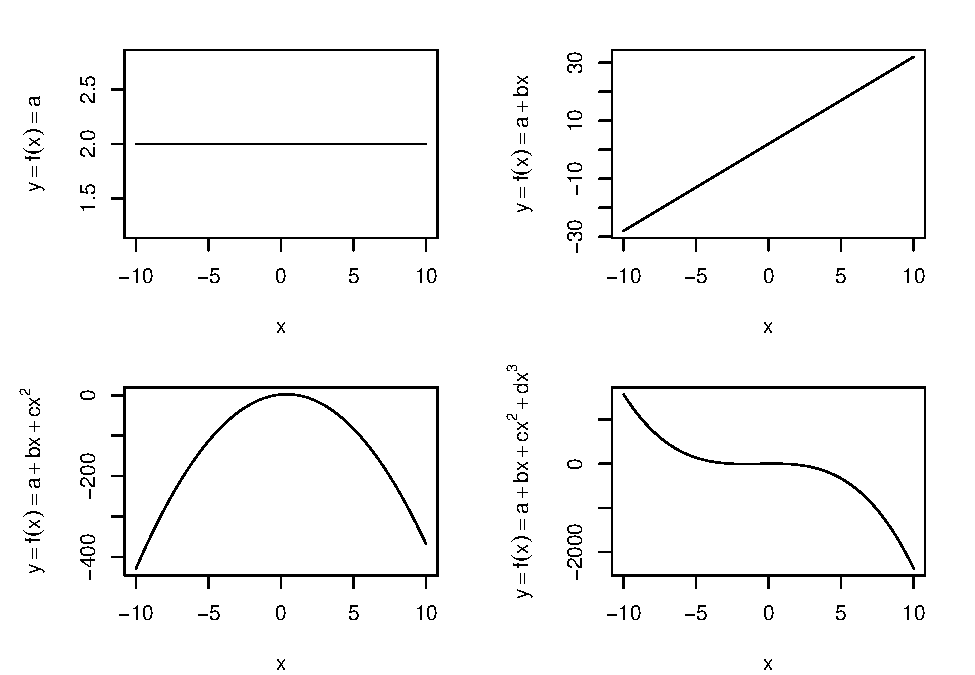
\includegraphics{bookdown-demo_files/figure-latex/fig-3-1-1.pdf}
\caption{\label{fig:fig-3-1}Лінійні та поліноміальні функції \(y = f(x)\) де \(f(x) = a\), \(f(x) = a + bx\), \(f(x) = a + bx + cx^2\), \(f(x) = a + bx + cx^2 + dx^3\) для \(a=2, b = 3, c = -4, d = -2\).}
\end{figure}

Більш поширеними є рівняння прямих ліній, які залежать від змінної \(x\). Найпростішим прикладом буде лінійне рівняння вигляду

\[y = f(x) = a + bx\]

де коефіцієнт \(a\) відповідає значенню \(y\) за \(x = 0\) та коефіцієнт \(b\) відповідає нахилу прямої, тобто відповідає на питання ``на скільки одиниць змінюється \(y\) за зміни \(x\) на одну одиницю''.

Наприклад, розгляньмо детальніше функцію \(y = f(x) = a + bx\), в якій \(a = 2, b = 3\) (Рис. \ref{fig:fig-3-2}):

\begin{figure}
\centering
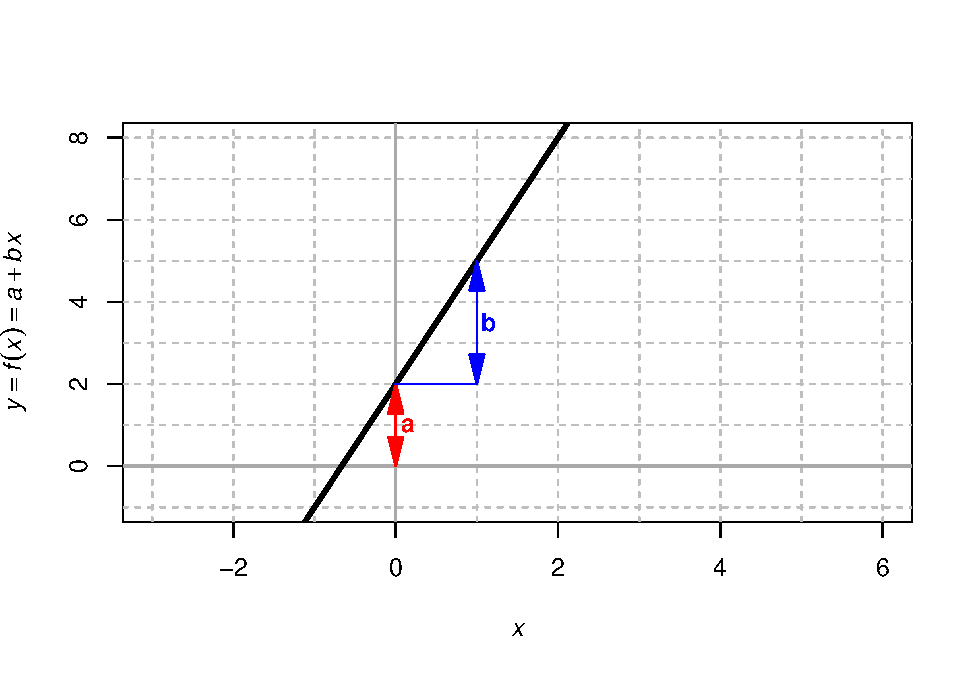
\includegraphics{bookdown-demo_files/figure-latex/fig-3-2-1.pdf}
\caption{\label{fig:fig-3-2}Зміст параметрів лінійної функції \(y = f(x) = a + bx\) для \(a=2, b = 3\).}
\end{figure}

Лінійна функція є окремим випадком поліноміальної функції, в якій ми буквенні коефіцієнти (\(a, b, c, \cdots\)) позначимо через індексовані коефіцієнти (\(\beta_0, \beta_1, \beta_2, \cdots\)):

\[p(x, m) = \beta_0 + \beta_1 x + \beta_2 x^2 + \cdots + \beta_m x^m\]

де \(m\) позначає ступінь полінома. Відтак, найпростіша функція перетину є поліноміальною функцією ступеню \(m = 0\), де \(p(x, m = 0) = \beta_0\), функція прямої є поліноміальною функцією ступеню \(m = 1\), де \(p(x, m = 1) = \beta_0 + \beta_1 x\), квадратична функція є поліноміальною ступеню \(m = 2\), де \(p(x, m = 2) = \beta_0 + \beta_1 x + \beta_2 x^2\) тощо.

Варто зазначити, що \(y\) може бути не лише лінійною функцією однієї змінної, скажімо, \(x\), а й комбінації \(m\) змінних \((x_1, x_2, x_3, \cdots, x_m)\), наприклад,

\[y = f(x_1, x_2, \cdots, x_m) = \beta_0 + \beta_1 x_1 + \beta_2 x_2 + \cdots + \beta_m x_m\]

В статистичному методі лінійної регресії одна зі змінних може являти собою трансформовану іншу змінну. Наприклад, якщо ми визначимо \(x_2\) як \(x_2 = (x_1)^2\), то квадратне рівняння можна визначити як лінійну комбінацію:

\[y = f(x_1, x_2) = \beta_0 + \beta_1 x_1 + \beta_2 x_2 = \beta_0 + \beta_1 x_1 + \beta_2 (x_1^2) = p(x_1, 2)\]

Таким чином, лінійна регресія може бути легко використана для моделювання нелінійних поліноміальних взаємозв'язків за рахунок трансформації змінних і їх використання в лінійних рівняннях.

\subsection{Логарифми}\label{logs}

Логарифмування є зворотним процесом то зведення в ступінь. Логарифм числа \(x\) із основою \(a\) є таким числом, зведення якого до ступеню \(a\) поверне число \(x\), тобто,

\[\log_a x = b\iff a^b = x\]

Найбільш поширеними є десятковий логарифм \(\log_{10}\) та натуральний логарифм \(\log_e\) де \(e\) -- число Ейлера \(e \approx 2.718\), константа, визначена як \(e = \lim\limits_{n \rightarrow \infty} (1 + \frac{1}{n})^n\).

В екології особливо поширений модифікований десятковий логарифм, оскільки чисельності організмів часто мають або низькі значення на кшталт \(0, 1, 2\), або дуже високі значення порядку сотень та тисяч, на рівні яких можна знехтувати одиничними особами\footnote{на рівні однієї, двох, трьох особин плюс-мінус одна особина багато чого змінює, в той час якщо є значення, скажімо, \(1234\), то плюс-мінус одна особина не вносить значної інформації; порівняйте \(\log_{10} 1 = 0\), \(\log_{10} 2 = 0.301\), \(\log_{10} 3 = 0.477\), і \(\log_{10} 1233 = 3.091\), \(\log_{10} 1234 = 3.091\), \(\log_{10} 1235 = 3.092\)}.

Модифікація логарифмічної трансформації в екології побудована таким чином, аби \(0\) відповідало \(0\) особин, \(1\) відповідало \(1\) особині, \(2\) відповідало \(10\) особинам, \(3\) відповідало \(100\) особинам, і так далі (\href{https://doi.org/10.1111/j.1461-0248.2006.00926.x}{Anderson et al.~2006}). Такої трансформації легко досягнути використовуючи функцію котра враховує факт, що логарифмування від'ємних значень та нуля неможливе (\(\log0 = -\infty\)):

\[f(x) = \begin{cases}
[\log_{10}(x)+1] \times \mathbb{I}_x(x > 0)\\
0 \times \mathbb{I}_x(x = 0)
\end{cases}\]

де \(\mathbb{I}_x(\cdot)\) є індикаторною функцією, котра приймає значення \(1\) якщо логічна умова \((\cdot)\) (тут, що \(x > 0\)) справджується.

Варто мати на увазі, що, в загальному, логарифмічне трансформування чисельностей не є оптимальною практикою, адже різниця між \(\log_{10}(0)\) та \(\log_{10}(1)\) така ж, як, наприклад, між \(\log_{10}(1000)\) та \(\log_{10}(10000)\), в той час як відсутність виду, котра призводить до отримання нульової чисельності, може передбачати набагато важливіші екологічні механізми порівняно із присутністю виду, котра призводить до не-нульової чисельності (\href{https://doi.org/10.1111/j.2041-210X.2010.00021.x}{O'Hara and Kotze 2010}).

Логарифми мають наступні властивості:

\[\log_a(xy) = \log_a(x) + \log_a(y)\]

\[\log_a(\frac{x}{y}) = \log_a(x) - \log_a(y)\]

\[\log_a(x^b) = b \log_a (x)\]

\[\log_a(x) = \frac{\log_b (x)}{\log_b (a)} \forall b\]

\subsection{Поширені математичні функції}\label{ux43fux43eux448ux438ux440ux435ux43dux456-ux43cux430ux442ux435ux43cux430ux442ux438ux447ux43dux456-ux444ux443ux43dux43aux446ux456ux457}

Кількість найпростіших математичних функцій доволі обмежена, однак, їх використання для трансформації змінних може бути кардинально різним. Трансформація даних може знадобитись пізніше, наприклад, для задоволення передбачень певних статистичних методів. Наприклад, лінійна регресія передбачає, що змінні розподілені нормально. В разі, якщо це не відповідає дійсності, одним із варіантів подальших дій є трансформування змінних певною функцією (наприклад, логарифмічно), за чого результуюча змінна може мати ближчий до нормального розподіл. Форми таких функцій наведені на Рис. \ref{fig:fig-3-3}.

\begin{figure}
\centering
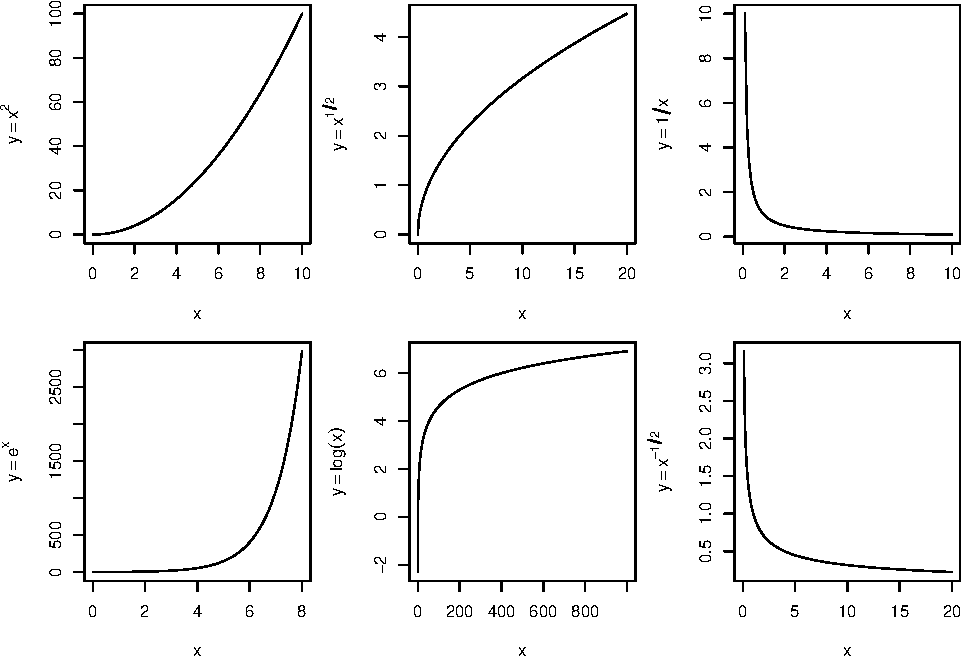
\includegraphics{bookdown-demo_files/figure-latex/fig-3-3-1.pdf}
\caption{\label{fig:fig-3-3}Графіки поширених функцій.}
\end{figure}

Варто також мати на увазі зворотні функції:

\begin{itemize}
\tightlist
\item
  поліноми та корені \(f(x) = x^2 \iff f^{-1}(y) = y^{1/2}\);
\item
  експоненти та логарифми \(f(x) = e^x \iff f^{-1}(y) = \log_e(y)\);
\item
  зворотні функції \(f(x) = 1/x \iff f^{-1}(y) = 1/y\).
\end{itemize}

\subsection{Властивості сум}\label{ux432ux43bux430ux441ux442ux438ux432ux43eux441ux442ux456-ux441ux443ux43c}

Суму позначають як \(\sum\limits_{i=m}^{n}f(x_i)\) де \(i\) є індексом сумації, \(x_i\) -- індексованою змінною, \(m\) -- нижня межа сумації, \(n\) -- верхня межа сумації. В програмуванні таку нотацію можна пояснити через цикл:

\begin{Shaded}
\begin{Highlighting}[]
\FunctionTok{sum}\NormalTok{(}\ControlFlowTok{for}\NormalTok{ (i }\ControlFlowTok{in}\NormalTok{ m}\SpecialCharTok{:}\NormalTok{n)\{}
  \FunctionTok{f}\NormalTok{(x[i])}
\NormalTok{\})}
\end{Highlighting}
\end{Shaded}

Суми мають наступні властивості

\[\sum\limits_{i=m}^{n}c\cdot f(x_i) = c \cdot \sum\limits_{i=m}^{n} f(x_i) \text{ } \forall \text{ } c : \text{const}\]

\[\sum\limits_{i=m}^{n} \left[ f(x_i) + g(x_i)\right] = \sum\limits_{i=m}^{n} f(x_i) + \sum\limits_{i=m}^{n} g(x_i)\]

\[\sum\limits_{i=m}^{n} f(x_i) = \sum\limits_{i=m}^{a} f(x_i) + \sum\limits_{i=a+1}^{n} f(x_i)\]

\[\left( \sum\limits_{i = m}^n x_i \right)\left( \sum\limits_{j = m}^n y_j \right) = \sum\limits_{i = m}^n \sum\limits_{j = m}^n (x_i y_j)\]

\[\sum \limits_{i=1}^n c = nc\]

\[\sum \limits_{i=0}^n \log i = \log n!\]

\[\sum \limits_{i=0}^n \binom{n}{i} = 2^n\]

\[\sum \limits_{i=0}^n \binom{n}{i} a^{n-i} b^i = (a+b)^n\]

\subsection{Властивості добутків}\label{ux432ux43bux430ux441ux442ux438ux432ux43eux441ux442ux456-ux434ux43eux431ux443ux442ux43aux456ux432}

Зміст нотації добутків подібний до суми. Суму позначають як \(\prod\limits_{i=m}^{n}f(x_i)\) де \(i\) є індексом добутку, \(x_i\) -- індексованою змінною, \(m\) -- нижня межа добутку, \(n\) -- верхня межа добутку. Для добутків притаманні наступні властивості:

\[\prod\limits_{i=1}^n x = x^n\]

\[\prod\limits_{i=1}^n x_i y_i = \left( \prod\limits_{i=1}^n x_i\right)\left( \prod\limits_{i=1}^n y_i\right)\]

\[\left( \prod\limits_{i=1}^n x_i \right)^a = \prod\limits_{i=1}^n x_i^a\]

\[\log_b \left[ \prod\limits_{i = m}^n f(x_i) \right] = \sum\limits_{i=m}^n \left[ \log_b f(x_i) \right]\]

\[\prod\limits_{i = m}^n [c \cdot f(x_i)] = c^{\sum_{i=m}^n f(x_i)}\]

\subsection{Диференціювання}\label{ux434ux438ux444ux435ux440ux435ux43dux446ux456ux44eux432ux430ux43dux43dux44f}

Диференціювання функції -- це процес знаходження похідної цієї функції. Похідна функції \(f(x)\) є такою функцією \(f'(x)\), котра описує зміну значення \(f(x)\) за зміни значення аргументу \(x\).

Наприклад, на Рис. \ref{fig:fig-3-2} зображено функцію прямої лінії \(f(x) = 2 + 3x\). В цьому випадку, приріст функції становить 3 одиниці \(y\) на одну одиницю \(x\), і цей приріст залишається незмінним за будь-якого значення \(x\), оскільки функція є прямою. Цей приріст і є похідною, отже, \(f'(x) = 3\).

А що щодо випадків, коли \(f(x)\) не є лінійною, що трапляється набагато частіше? В такому випадку, приріст \(f(x)\) залежить від значення \(x\), тобто \(f'(x)\) теж є функцією із аргументом \(x\). Власне, знаходження цієї функції і є метою диференціювання. Формально, визначення похідної являє собою зміну \(f(x)\) за найменшої різниці \(x\).

Наприклад, визначмо функцію \(f(x) = -5x + x^3\) (Рис. \ref{fig:fig-3-4}):

\begin{figure}
\centering
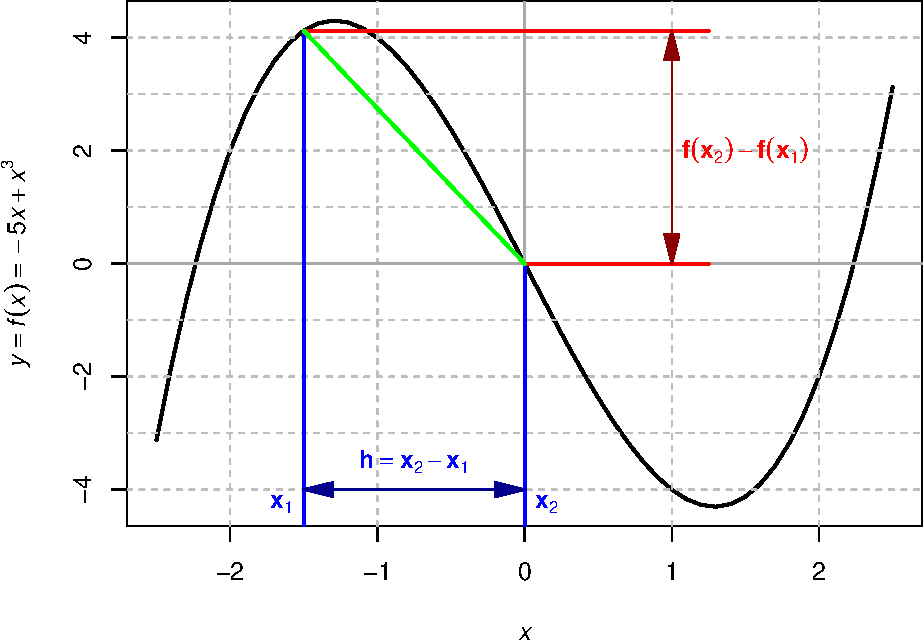
\includegraphics{bookdown-demo_files/figure-latex/fig-3-4-1.pdf}
\caption{\label{fig:fig-3-4}Функція \(f(x) = -5x + x^3\). Приріст цієї функції між \(x_1\) та \(x_2 = x_1 + h\) складає \(\frac{f(x_1 + h) - f(x_1)}{h}\).}
\end{figure}

Для цієї функції, похідна буде такою функцією із аргументом \(x\), котра описуватиме \(f(x_2) - f(x_1)\) на зміну \((x_2 - x_1)\). На Рис. \ref{fig:fig-3-4} показано зміну \(f(x)\) для \(x_2 = 0, x_1 = -1.5\), тобто \(h = x_2 - x_1 = 1.5\), де значення функції становить \(f(x_2) = -5 \cdot 0 + 0^3 = 0\), \(f(x_1) = -5 \cdot (-1.5) + (-1.5)^3 = 4.125\), отже, \(f(x_2) - f(x_1) = f(x_1+h) - f(x_1) = -4.125\), а темп цієї зміни на одиницю \(x\) становить \(\frac{f(x_1 + h) - f(x_1)}{h} = \frac{-4.125}{1.5} = -2.75\).

На тій частині функції, котра відповідає \(x_1, x_1+h\), отримане значення темпу зміни може не цілком відповідати реальній картині. Ми бачимо, що функція трішки зростає після \(x_1\), потім спадає, і взагалі є нелінійною, але обчислене значення \(\frac{f(x_1 + h) - f(x_1)}{h} = \frac{-4.125}{1.5} = 2.75\) відповідає ситуації, коли розглянута функція є прямою лінією (зображено зеленим). Аби відобразити справжню природу зміни значення функції, необхідно зменшити значення \(h\) до найменшого можливого значення. Відтак, класичне визначення похідної -- це така функція із аргументом \(x\), що описує темп зміни \(\frac{f(x+h) - f(x)}{h}\) за найменшої зміни \(h\):

\[f'(x) = \frac{df(x)}{dx} = \lim\limits_{h \rightarrow 0}\frac{f(x+h) - f(x)}{h}\]

де позначення похідної через \(\frac{df(x)}{dx}\) інтуїтивно вказує на її природу, якщо позначити зміну значення змінної через \(d\): зміна значення \(f(x)\) поділена на зміну значення \(x\). Похідну варто сприймати як приріст функції, котрий буде позитивним коли функція зростає, негативним коли функція спадає, і дорівнює нулю коли функція залишається сталою (таке можливе або якщо функція є прямою горизонтальною лінією, або коли в точках перегину, коли функція перестає зростати і починає спадати або навпаки).

Похідні мають наступні властивості, котрі допомагають розрахувати їх для будь-якої неперервної функції:

\[\frac{d}{dx}a = 0\]

\[\frac{d}{dx}ax = a\]

\[\frac{d}{dx} x^a = ax^{a-1}\]

\[\frac{d}{dx} e^x = e^x\]

\[\frac{d}{dx} a^x = a^x \ln (a) \text{ } \forall \text{ } a>0\]

\[\frac{d}{dx} \ln (x) = \frac{1}{x} \text{ } \forall \text{ } x>0\]

\[\frac{d}{dx} \log_a(x) = \frac{1}{x \ln(a)}\]

В диференціюванні складних функцій (функцій, котрі складаються з інших функцій, наприклад, \(f(\cdot)\) і \(g(\cdot)\)) керуються наступними правилами:

\[\frac{d}{dx} \left( af(x) + b g(x) \right) = a \frac{d}{dx}f(x) + b \frac{d}{dx}g(x) \iff (af(x) + bg(x))' = af'(x) + bg'(x)\]

\[\frac{d}{dx}(f(x)g(x)) = \frac{df(x)}{dx} g(x) + f(x) \frac{dg(x)}{dx} \iff (f(x)g(x))' = f'(x)g(x) + f(x)g'(x)\]

\[\frac{d}{dx} \left( \frac{f(x)}{g(x)}\right) = \frac{\frac{df(x)}{dx}g(x) - f(x) \frac{dg(x)}{dx}}{g(g(x))} \iff \left( \frac{f(x)}{g(x)} \right)' = \frac{f'(x)g(x) - f(x)g'(x)}{g^2(x)}\]

і для функції функції \(f(x) = h(g(x))\),

\[\frac{df(x)}{dx} = \frac{dh(g(x))}{dg(x)} \cdot \frac{dg(x)}{dx} \iff f'(x) = h'(g(x)) \cdot g'(x)\]

Оскільки похідна є функцією сама по собі, її також можна диференціювати (тобто знайти \(n\)-ну похідну, або похідну \(n\)-ного порядку). Наприклад, для функції \(f(x) = -5x + x^3\),

\[\begin{cases}
\frac{d}{dx}f(x) = -5 + 3x^2 \\
\frac{d^2}{dx}f(x) = 6x \\
\frac{d^3}{dx}f(x) = 6 \\
\frac{d^4}{dx}f(x) = 0
\end{cases}\]

\begin{figure}
\centering
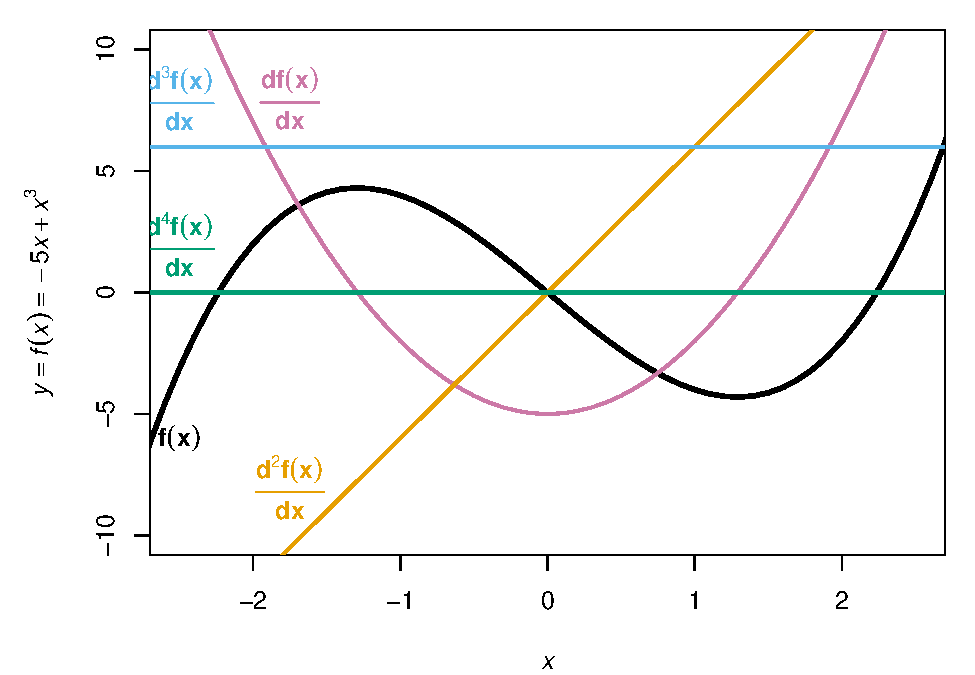
\includegraphics{bookdown-demo_files/figure-latex/fig-3-5-1.pdf}
\caption{\label{fig:fig-3-5}Функція \(f(x) = -5x + x^3\) та її похідні.}
\end{figure}

\subsection{Інтегрування}\label{ux456ux43dux442ux435ux433ux440ux443ux432ux430ux43dux43dux44f}

Інтегрування функції \(f(x)\) -- це процес знаходження такої функції \(F(x)\), похідна якої являє собою функцію \(f(x)\):

\[\frac{d}{dx}F(x) = f(x) \iff \int f(x) dx = F(x) + C\]

де \(C\) -- це будь-яка константа (оскільки похідна константи дорівнює нулю, ця константа не впливає на результат диференціювання).

Інтеграл є, певною мірою, континуальний аналог суми: якщо означення суми оперує дискретними значеннями \(i: i = 1, 2, 3, \cdots, n\), то інтеграл, подібно до похідних, розраховується для найменших можливих інтервалів аргументу функції \(x\).

\textbf{\emph{Невизначений інтеграл}} функції \(f(x)\) \(\int f(x)dx = F(x)\) має зміст як функція, похідна якої дорівнює вихідній функції \(f(x)\). Водночас, \textbf{\emph{визначений інтеграл}} \(\int\limits_a^b f(x) dx = F(b) - F(a)\) часто використовується для знаходження площі під кривою \(f(x)\), що обмежена значеннями \(a\) і \(b\).

В разі, якщо аналітичне знаходження невизначеного інтегралу складне або неможливе, корисним може видатись Рейманівське визначення визначеного інтегралу:

\[\int\limits_a^b f(x) dx = F(a) - F(b) = \sum\limits_{i=1}^n [F(x_i) - F(x_{i-1})]\]

де \([F(x_i) - F(x_{i-1})]\) є площею прямокутника, обмеженого функцією \(f(x)\) і дуже маленьким інтервалом \([x_{i-1}, x_i)\) (Рис. \ref{fig:fig-3-6}).

\begin{figure}
\centering
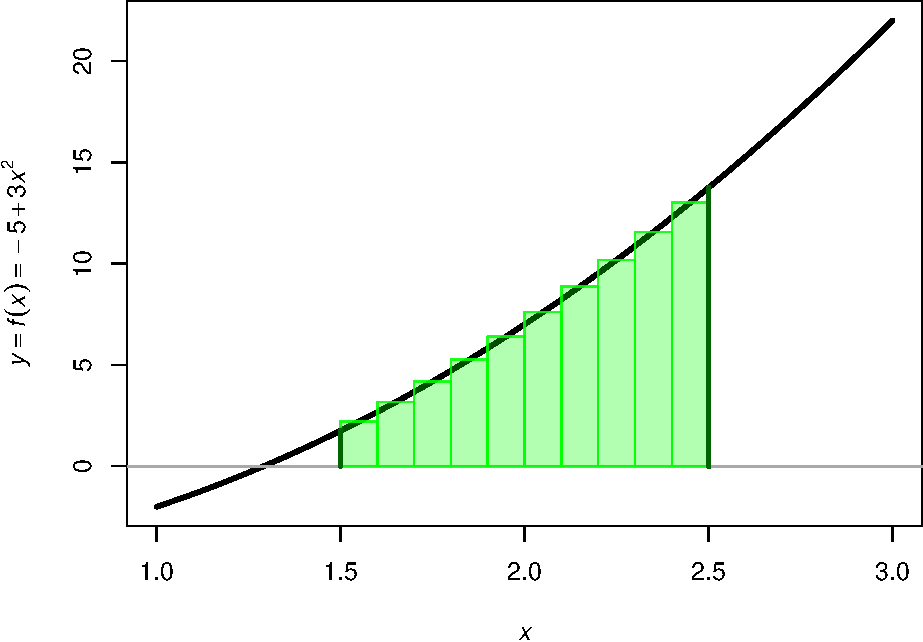
\includegraphics{bookdown-demo_files/figure-latex/fig-3-6-1.pdf}
\caption{\label{fig:fig-3-6}Знаходження визначеного інтеграла як Рейманівську суму функції \(f(x) = -5 + 3x^2\).}
\end{figure}

Якщо, наприклад, шукати площу під кривою як на Рис. \ref{fig:fig-3-6} поділом інтервалу між \(a = 1.5\), \(b = 2.5\) на \(10\) прямокутників (хоча їх може бути скільки завгодно), то це нескладно обчислити за допомогою R:

\begin{Shaded}
\begin{Highlighting}[]
\NormalTok{f }\OtherTok{\textless{}{-}} \ControlFlowTok{function}\NormalTok{(x) }\SpecialCharTok{{-}}\DecValTok{5} \SpecialCharTok{+} \DecValTok{3}\SpecialCharTok{*}\NormalTok{x}\SpecialCharTok{\^{}}\DecValTok{2}
\FunctionTok{sum}\NormalTok{(}\FunctionTok{sapply}\NormalTok{(}\FunctionTok{seq}\NormalTok{(}\FloatTok{1.5}\NormalTok{, }\FloatTok{2.4}\NormalTok{, }\FloatTok{0.1}\NormalTok{)}\SpecialCharTok{+}\FloatTok{0.05}\NormalTok{, }\ControlFlowTok{function}\NormalTok{(x) }\FloatTok{0.1}\SpecialCharTok{*}\FunctionTok{f}\NormalTok{(x)))}
\end{Highlighting}
\end{Shaded}

\begin{verbatim}
## [1] 7.2475
\end{verbatim}

Із прикладу на Рис. \ref{fig:fig-3-5} ми знаємо, що функція \(f(x) = -5 + 3x^2\) є першою похідною функції \(F(x) = -5x + x^3\), яка, за визначенням, є невизначеним інтегралом \(\int f(x)dx\). Відповідно,

\[
\begin{aligned}
  \int\limits_{1.5}^{2.5}-5 + 3x^2 dx = F(2.5) - F(1.5) = \left[ -5x + x^3 \right]_{1.5}^{2.5} = \\ [-5 \cdot 2.5 + 2.5^3] - [-5 \cdot 1.5 + 1.5^3] = 3.125 - (-4.125) = 7.25 \simeq 7.2475
\end{aligned}
\]

Типові інтеграли мають наступні значення:

\[\int x^a dx = \frac{x^{a+1}}{a+1} + C \text{ } \forall \text{ } a \neq -1\]

\[\int x^{-1} dx = \int \frac{dx}{x} = \ln(|x|) + C\]

\[\int axdx = ax + C\]

\[\int \frac{1}{ax + b}dx = \frac{1}{a} \ln(|ax+b|) + C\]

\[\int \ln(x) dx = x \ln(x) -x + C\]

\[\int e^x dx = e^x + C\]

Інтегралам притаманні наступні властивості:

\[\int \limits_a^b c f(x) dx = c \int \limits_a^b f(x) dx\]

\[\int \limits_a^b f(x) + g(x) dx = \int \limits_a^b f(x) dx + \int \limits_a^b g(x) dx\]

\[\int \limits_a^a f(x)dx = 0\]

\[\int \limits_a^b f(x)dx = -\int \limits_b^a f(x)dx\]

\[\int \limits_a^c f(x)dx = \int \limits_a^b f(x)dx + \int \limits_b^c f(x)dx \text{ } \forall \text{ } a < b < c\]

Для інтегрування складних функцій використовують наступні техніки:

\begin{itemize}
\tightlist
\item
  інтегрування підстановкою
\end{itemize}

\[\int \limits_a^b f(g(x)) g'(x)dx = \int \limits_{g(a)}^{g(b)} f(u) du\]

де \(u = g(x)\), \(du = g'(x)dx\)

\begin{itemize}
\tightlist
\item
  інтегрування частинами
\end{itemize}

\[\int u (dv) = uv - \int v (du) \iff \int f(x)g'(x)dx = f(x)g(x) - \int f'(x) g(x) dx\]

де \(v = \int dv\).

В цілому, в екології рідко коли потрібно аналітично вирішити інтеграл чи похідну, однак, розуміння \emph{змісту} цих операцій необхідне для подальшого розуміння статистичних підходів. В рідкісних випадках, коли необхідно вирішити певний інтеграл, має сенс скористатися онлайн-сервісами на кшталт \href{https://www.integral-calculator.com/}{integral-calculator.com} або розрахувати значення визначеного інтегралу ітеративно за допомогою Рейманівської суми, як показано вище. Варто також мати на увазі, що деякі функції неможливо або дуже складно аналітично проінтегрувати.

\section{Лінійна алгебра}\label{matrices}

\subsection{Визначення матриці}\label{ux432ux438ux437ux43dux430ux447ux435ux43dux43dux44f-ux43cux430ux442ux440ux438ux446ux456}

Матриця є двовимірним набором значень, що позначається як

\[\textbf{A} = \begin{bmatrix}
a_{1, 1} & a_{1,2} & \cdots & a_{1, n}\\
a_{2, 1} & a_{2,2} & \cdots & a_{2, n}\\
\vdots & \vdots & a_{i,j} & \vdots \\
a_{m, 1} & a_{m,2} & \cdots & a_{m, n}
\end{bmatrix}\]

в якій \(i: 1, 2, \cdots, m-1, m\) позначає індекс рядка елементу і \(j: 1, 2, \cdots, n-1, n\) позначає індекс колонки елементу \(a_{i, j}\). В цій книзі матриці як об'єкти позначатимуться жирними великими літерами і визначатимуться як матриці в квадратних дужках, але варто мати на увазі, що позначення іноді варіюють в різних джерелах.

Розмірність матриці визначається кількістю рядків \(m\) та кількістю колонок \(n\). Якщо один із цих вимірів дорівнює одиниці, матриця являє собою \textbf{\emph{вектор}} -- послідовність значень. Поняття вектору важливе для розуміння оперування даними, адже спостереження (рядки) та параметри (колонки) в масиві даних є векторами розмірністю \(m \times 1\) або \(1 \times n\). Вектори позначаються як \(\vec{a}\).

В подальшому матриці визначені як жирні літери (напр., \(\mathbf{A}\)), а елементи матриці -- як індексовані літери \(a_{i,j}\), або \([\mathbf{A}]_{i,j}\).

\subsection{Трансформації матриць}\label{ux442ux440ux430ux43dux441ux444ux43eux440ux43cux430ux446ux456ux457-ux43cux430ux442ux440ux438ux446ux44c}

\textbf{\emph{Додавання матриць}}, якщо обидві матриці мають ідентичну розмірність, є доволі очевидним, адже додаються елементи із ідентичними індексами. Наприклад, \(\mathbf{A}+\mathbf{B} = a_{i,j}+b_{i, j}\).

Наприклад, якщо

\[\mathbf{A} = \begin{bmatrix}
a_{1, 1} & a_{1,2} & \cdots & a_{1, n}\\
a_{2, 1} & a_{2,2} & \cdots & a_{2, n}\\
\vdots & \vdots & a_{i,j} & \vdots \\
a_{m, 1} & a_{m,2} & \cdots & a_{m, n}
\end{bmatrix},
\mathbf{B} = \begin{bmatrix}
b_{1, 1} & b_{1,2} & \cdots & b_{1, n}\\
b_{2, 1} & b_{2,2} & \cdots & b_{2, n}\\
\vdots & \vdots & b_{i,j} & \vdots \\
b_{m, 1} & b_{m,2} & \cdots & b_{m, n}
\end{bmatrix}\]

тоді

\[\mathbf{A} + \mathbf{B} = \begin{bmatrix}
a_{1, 1}+b_{1, 1} & a_{1,2}+b_{1,2} & \cdots & a_{1, n}+b_{1, n}\\
a_{2, 1}+b_{2, 1} & a_{2,2}+b_{2,2} & \cdots & a_{2, n}+b_{2, n}\\
\vdots & \vdots & a_{i,j}+b_{i,j} & \vdots \\
a_{m, 1}+b_{m, 1} & a_{m,2}+b_{m,2} & \cdots & a_{m, n}+b_{m, n}
\end{bmatrix}\]

Подібно до додавання, \textbf{\emph{скалярне множення}} матриць полягає в отриманні добутку константи із кожним елементом матриці:

\[c \cdot \mathbf{A} = c \cdot a_{i, j} = \begin{bmatrix}
c \cdot a_{1, 1} & c \cdot a_{1,2} & \cdots & c \cdot a_{1, n}\\
c \cdot a_{2, 1} & c \cdot  a_{2,2} & \cdots & c \cdot a_{2, n}\\
\vdots & \vdots & c \cdot a_{i,j} & \vdots \\
c \cdot a_{m, 1} & c \cdot a_{m,2} & \cdots & c \cdot a_{m, n}
\end{bmatrix}\]

Нарешті, \textbf{\emph{транспонування}} матриці полягає в заміні індексування рядків та колонки і навпаки, \(i \rightarrow j, j \rightarrow i\), тобто,

\[\mathbf{A'} = \mathbf{A^T} = a'_{j, i} \text{ } \forall \text{ } \mathbf{A} = a_{i, j}\]

\subsection{Операції над матрицями}\label{ux43eux43fux435ux440ux430ux446ux456ux457-ux43dux430ux434-ux43cux430ux442ux440ux438ux446ux44fux43cux438}

\textbf{\emph{Множення матриць}} є дещо складнішим, і загальним правилом є те, що для матриць \(A\) розміром \(m \times n\) і \(B\) розміром \(n \times p\) добуток складатиме матрицю розміром \(m \times p\) із елементами, що відповідають сумі добутків рядків \(A\) та колонок \(B\), тобто елемент добутку матриць із індексами \(i, j\) складатиме (\href{https://books.google.com/books/about/Linear_Algebra.html?id=P8BZzAEACAAJ}{Bogacki 2019}) (Рис. \ref{fig:fig-3-7})

\[[\mathbf{AB}]_{i, j} = \sum \limits_{r=1}^n (a_{i,r} b_{r, j}) = a_{i,1} b_{1, j} + a_{i, 2}b_{2, j} + \cdots + a_{i, n}b_{n, j}\]

\begin{figure}
\centering
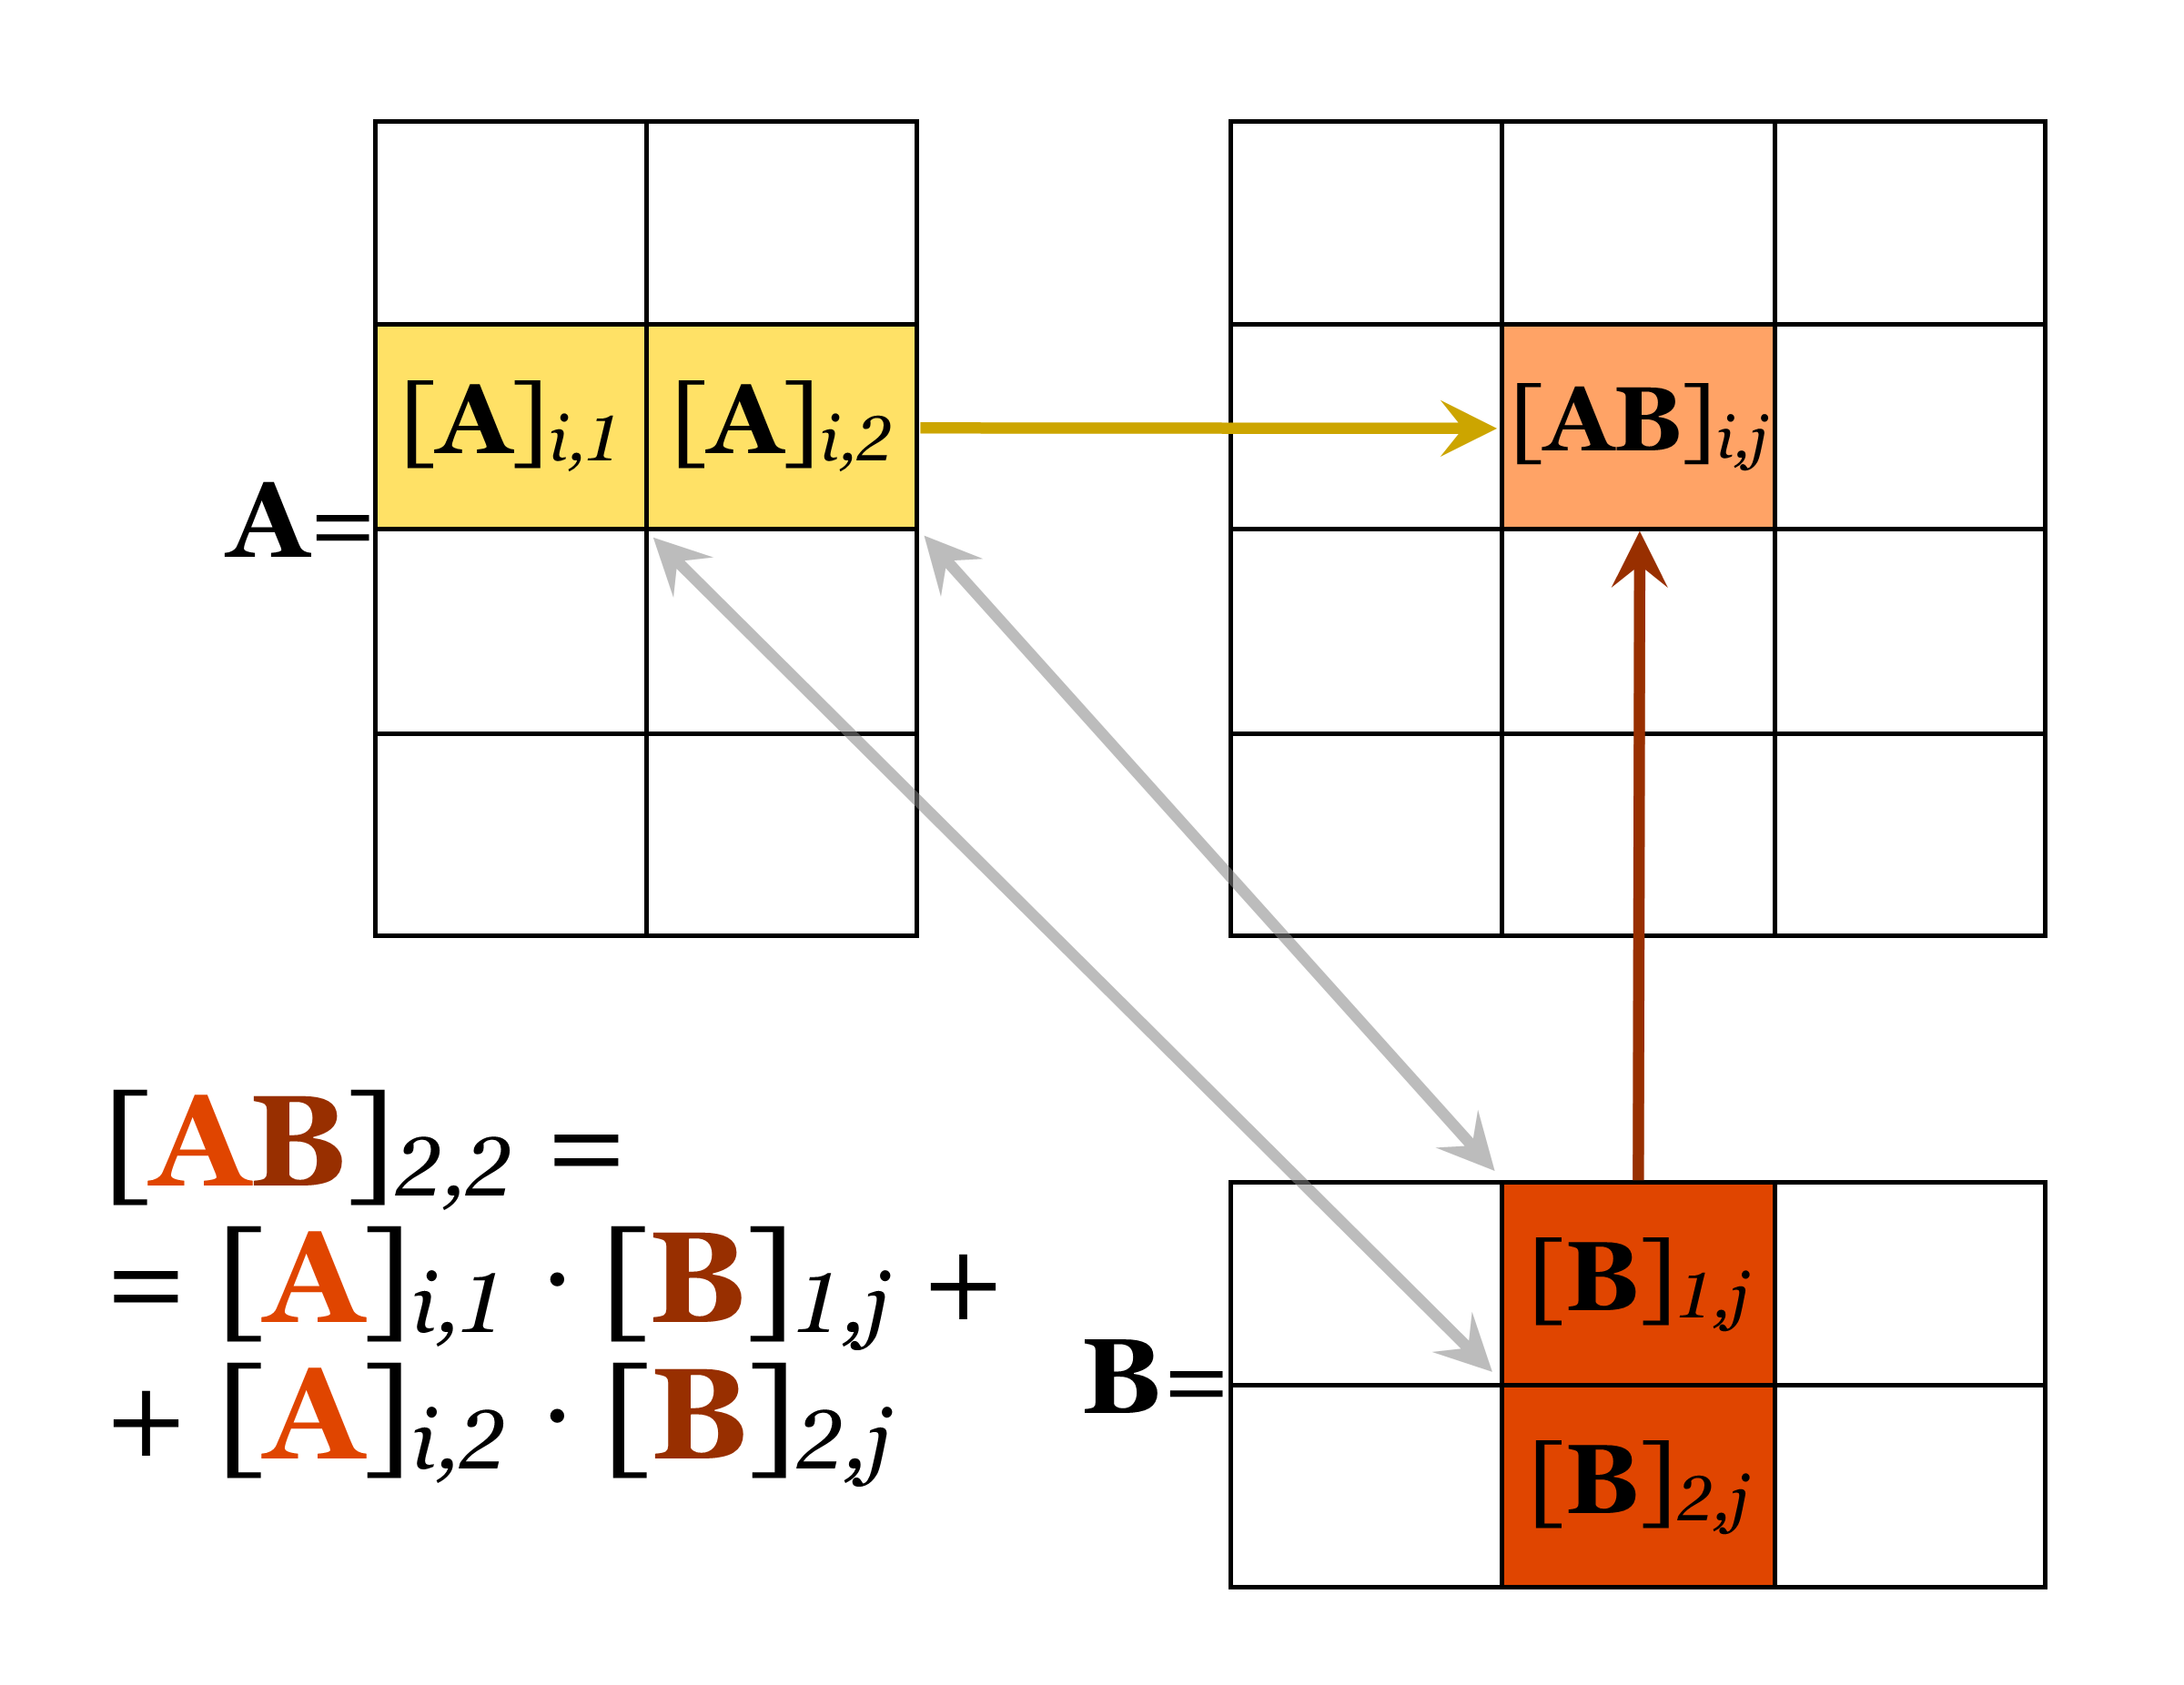
\includegraphics{images/matrices.png}
\caption{\label{fig:fig-3-7}Знаходження значення елементу добутку матриць \(\mathbf{A}\) і \(\mathbf{B}\).}
\end{figure}

Для добутків матриць властиво, що

\[\mathbf{AB} \neq \mathbf{BA}\]

\[(\mathbf{AB})\mathbf{C} = \mathbf{A}(\mathbf{BC})\]

\[(\mathbf{A+B})\mathbf{C} = \mathbf{AC} + \mathbf{BC}\]

\[\mathbf{C}(\mathbf{A+B}) = \mathbf{CA} + \mathbf{CB}\]

Очевидно, що якщо множення матриць можливе, то можливо також і звести матрицю в ступінь, наприклад,

\[\mathbf{A}^3 = (\mathbf{AA})\mathbf{A}\]

Уявімо квадратну \textbf{\emph{одиничну матрицю}} \(\mathbf{I}_n\) розміром \(n \times n\), де

\[\mathbf{I}_n = \begin{bmatrix}
1 & 0 & 0 & \cdots & 0\\
0 & 1 & 0 & \cdots & 0\\
0 & 0 & 1 & \cdots & 0\\
\vdots & \vdots & \vdots & \ddots  &\vdots \\
0 & 0 & 0 & \cdots & 1
\end{bmatrix}\]

тобто всі, крім діагональних, елементи матриці дорівнюють нулю. Тоді

\[\mathbf{AB} = \mathbf{I}_n = \mathbf{BA}\]

отже, \(\mathbf{B}\) є \textbf{\emph{оберненою матрицею}} \(\mathbf{A}\):

\[\mathbf{B} = \mathbf{A}^{-1}\]

\[\mathbf{AA^{-1}} = \mathbf{I}_n\]

\[\mathbf{A}^0 = \mathbf{I}_n\]

Очевидно, що \textbf{не} для будь-якої матриці може існувати обернена матриця.

Подібно до математичних функцій, \textbf{\emph{лінійні трансформації}} можуть приймати вектори чи матриці в якості аргументу:

\[F: \mathbb{R}^n \rightarrow \mathbb{R}^m \text{ якщо}\]

\[F(\vec{u} + \vec{v}) = F(\vec{u}) + F(\vec{v}) \text{ } \forall \text{ } \vec{u}, \vec{v}\]

\[F(c \vec{u}) = c F(\vec{u}) \text{ } \forall \text{ } \vec{u}, c\]

\[F(c_1 \vec{u_1} + \cdots + c_k \vec{u_k}) = c_1 F(\vec{u_1}) + \cdots + c_k F(\vec{u_k})\]

\[F: \mathbb{R}^n \rightarrow \mathbb{R}^m \iff \exists \mathbf{A}: F(\vec{v}) = \mathbf{A} \vec{v}, \mathbf{A} = a_{i, j}, 1 < i<m, 1 < j < n\]

\subsection{Детермінант, власні вектори, та власне значення}\label{ux434ux435ux442ux435ux440ux43cux456ux43dux430ux43dux442-ux432ux43bux430ux441ux43dux456-ux432ux435ux43aux442ux43eux440ux438-ux442ux430-ux432ux43bux430ux441ux43dux435-ux437ux43dux430ux447ux435ux43dux43dux44f}

\textbf{\emph{Детермінант}} визначається (\href{https://books.google.com/books/about/Linear_Algebra.html?id=P8BZzAEACAAJ}{Bogacki 2019}) для матриці \(1 \times 1\) \(\mathbf{A} = [a_{1, 1}]\) як

\[\det \mathbf{A} = a_{1, 1}\]

і для більших квадратних матриць розміром \(n \times n\) рекурсивно

\[\det \mathbf{A} = \sum \limits_{j=1}^n (-1)^{1+j} a_{1, j} \det \mathbf{M}_{1,j}\]

де \(\mathbf{M}_{i,j}\) є підматрицею від \(\mathbf{A}\) розміром \((n - 1) \times (m - 1)\) із видаленими рядком \(i\) і колонкою \(j\), тобто,

\[\det \mathbf{A} = a_{1,1} \det \mathbf{M}_{1,1} - a_{1,2} \det \mathbf{M}_{1,2} + a_{1,3} \det \mathbf{M}_{1,3} - \cdots + (-1)^{1+n} a_{1, n} \det \mathbf{M}_{1,n}\]

Для матриці \(\mathbf{A}\) розміром \(2 \times 2\), наприклад,

\[\det \mathbf{A} = \det \begin{bmatrix}
a_{1, 1} & a_{1, 2} \\
a_{2, 1} & a_{2, 2}
\end{bmatrix} = a_{1, 1} \cdot a_{2, 2} - a_{1, 2} \cdot a_{2, 1}\]

\subsection{Геометричний зміст матриць}\label{matrices_art}

Технічні визначення операцій над матрицями можуть видаватись надмірно деталізованими і неінтуїтивними правилами, котрі просто необхідно завчити. Однак, всі ці правила мають очевидний геометричний зміст, котрий рідко використовують в поясненнях базової теорії матриць \href{https://youtube.com/playlist?list=PLZHQObOWTQDPD3MizzM2xVFitgF8hE_ab}{3Blue1Brown 2023}.

В першу чергу, необхідно зрозуміти поняття вектора. В багатьох чисельних методах і, зокрема, в програмному середовищі R, векторами звуться скінченні ряди чисел, наприклад, змінна в наборі даних. Однак, зі шкільної програми математики можна пригадати, що векторами є і спрямовані відрізки. Наприклад, якщо позначити вектор \(\vec{a}\) як \(\vec{a} = (1, 2)\), то ряд чисел \((1, 2)\) можна зобразити як такий вектор, що починається з координат \((x_0 = 0, y_0 = 0)\) і закінчується координатами \((x_1 = 1, y_1 = 2)\).

Уявімо простір таких векторів. З попереднього параграфу можна помітити, що хоча й, формально, вектор має дві точки (в двовимірному просторі це \((x_0, y_0)\) та \((x_1, y_1)\)), для кожного вектору одна з точок буде однаковою: \((x_0 = 0, y_0 = 0)\). Відтак, ми не втратимо ніякої інформації, якщо для багатьох векторів ми забудемо про початкові точки і визначимо лише кінцеві точки. У двовимірному просторі можна визначити скільки завгодно векторів/точок \(\vec{v_1} = (x_{1, 1}, y_{1, 1}), \vec{v_2} = (x_{1, 2}, y_{1, 2}), \cdots, \vec{v_i} = (x_{1, i}, y_{1, i})\), але, звісно, це справджуватиметься і для одного виміру (\(\vec{v_1} = (x_{1, 1}), \vec{v_2} = (x_{1, 2}), \cdots, \vec{v_i} = (x_{1, i})\)), і для трьох вимірів (\(\vec{v_1} = (x_{1, 1}, y_{1, 1}, z_{1, 1}), \vec{v_2} = (x_{1, 2}, y_{1, 2}, z_{1, 2}), \cdots, \vec{v_i} = (x_{1, i}, y_{1, i}, z_{1, i})\)), і для будь-якої скінченної кількості вимірів. В структурі даних, відтак, хоча й ряди чисел є векторами, ми можемо уявити кожне спостереження як точку у просторі параметрів цього спостереження (т. зв. точка даних, або data point, що ж еквівалентним одиночному спостереженню).

Для простору векторів, матриця є лінійною трансформацією. Тобто, якщо помножити координати точки (або вектору, що є тим самим) на матрицю, то на виході ми отримаємо інший лінійний вектор. Подібно до математичної функції, ми можемо застосувати лінійну трансформацію до всього простору, і отримаємо інший простір, в котрому точки знаходяться та пропорційній до вихідного простору відстані одна від одної, а прямі між точками залишаються прямими\footnote{очевидно, ці дві умови не завжди можуть справджуватися, у випадку чого трансформація не є лінійною}.

Пригадаймо правила множення матриць. Для цього потрібно кожен вектор уявити у вигляді матриці. Наприклад, для вектору \[\vec{a} = (x_1 = 1, y_1 = 2) = \begin{bmatrix} 
x_1 = 1 \\ 
y_1 = 2 \end{bmatrix} = \begin{bmatrix}
1 \\
2 \end{bmatrix}\]

застосуймо матрицю

\[\mathbf{A} = \begin{bmatrix}
1 & 2 \\
3 & 4
\end{bmatrix}\]

\[
\mathbf{A} \vec{a} = \begin{bmatrix}
1 & 2 \\
3 & 4
\end{bmatrix} \cdot \begin{bmatrix}
1 \\ 2 
\end{bmatrix}= \begin{bmatrix}
1 \cdot 1 + 2 \cdot 2 \\
1 \cdot 3 + 2 \cdot 4
\end{bmatrix} = \begin{bmatrix}
5 \\ 11
\end{bmatrix}
\]

Тобто після застосування лінійної трансформації до вектору ми отримуємо вектор такої ж розмірності, при чому ця лінійна трансформація може бути застосована для будь-якого вектору такої розмірності. Тож матриця \(\mathbf{A}\) відповідає лінійній трансформації, зображеній на Рис. \ref{fig:fig-3-8}.

\begin{figure}
\centering
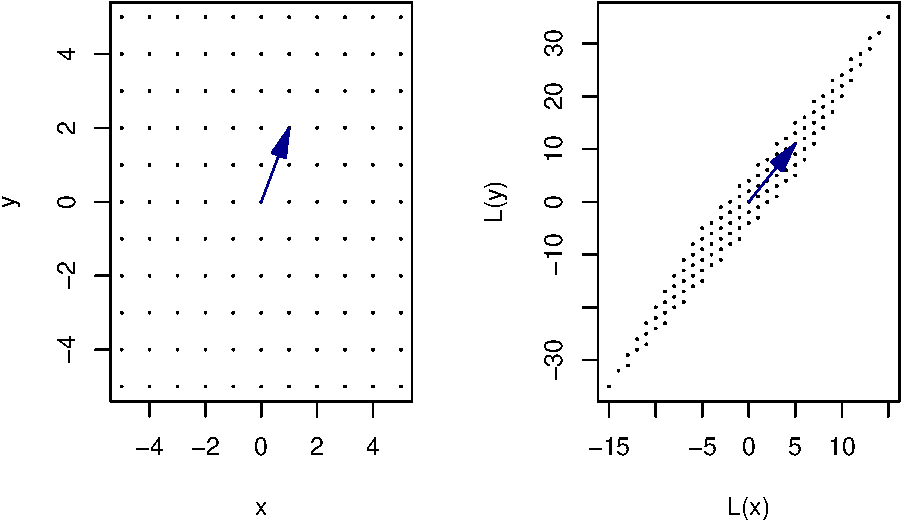
\includegraphics{bookdown-demo_files/figure-latex/fig-3-8-1.pdf}
\caption{\label{fig:fig-3-8}Матриця \(\mathbf{A} = \begin{bmatrix} 1 & 2 \\ 3 & 4 \end{bmatrix}\) як лінійна трансформація простору. Вектор \(\vec{a} = \begin{bmatrix} 1 \\ 2 \end{bmatrix}\) є лише частиною цього простору.}
\end{figure}

Загалом, для всякого двовимірного простору можна уявити два незалежні базові вектори: \(\hat{i} = \begin{bmatrix} 1 \\ 0 \end{bmatrix}\) й \(\hat{j} = \begin{bmatrix} 0 \\ 1 \end{bmatrix}\). Тоді будь-який вектор \(\vec{v}\) є сумою векторів, що відображають добутки певної константи \(a\) та \(\hat{i}\) й \(b\) та \(\hat{j}\): \(\vec{v} = a \hat{i} + b \hat{j}\), а, відтак, всяку лінійну трансформацію \(L(\cdot)\) можна виразити у вигляді \[L(\vec{v}) = a L(\hat{i}) + b L(\hat{j})\]

відтак, лінійна трансформація вектору \(\begin{bmatrix} x \\ y \end{bmatrix} \rightarrow L \left( \begin{bmatrix} x \\ y \end{bmatrix} \right)\) є тотожною лінійній трансформації базових векторів, шкалованих на певні константи для базових векторів:

\[L \left( \begin{bmatrix} x \\ y \end{bmatrix} \right) = x[L (\hat{i})] + y[L(\hat{j})] = \begin{bmatrix} x L(1) & xL(0) \\ y L(0) & y L(1) \end{bmatrix}\]

Тобто сутність квадратної матриці як репрезентації лінійної трансформації -- це сукупність координат, на які припадають базові вектори після лінійної трансформації. Для попереднього прикладу \(\mathbf{A} = \begin{bmatrix} 1 & 2 \\ 3 & 4 \end{bmatrix}\), зокрема, \(L(\hat{i})\) матиме координати \((1, 3)\), а \(L(\hat{j})\) -- \((2, 4)\).

Якщо розглядати матрицю як носій інформації про лінійну трансформацію, то множення матриць є нічим іншим, як застосуванням лінійної трансформації до лінійної трансформації. Тобто, якщо уявити дві лінійні трансформації \(L_1\) та \(L_2\) такі що

\[L_2 \left( L_1 \left( \begin{bmatrix} 
x \\ 
y 
\end{bmatrix} \right) \right) = 
\begin{bmatrix} 
a & c \\ 
b & d
\end{bmatrix}
\left( 
\begin{bmatrix} 
e & g \\ 
f & h
\end{bmatrix}
\begin{bmatrix} 
x \\ 
y 
\end{bmatrix}
\right) = 
\left( 
\begin{bmatrix} 
a & c \\ 
b & d
\end{bmatrix}
\begin{bmatrix} 
e & g \\ 
f & h
\end{bmatrix}
\right)
\begin{bmatrix} 
x \\ 
y 
\end{bmatrix} = 
\begin{bmatrix} 
ae + bg & af + bh \\ 
ce + dg & cf + dh
\end{bmatrix}
\begin{bmatrix} 
x \\ 
y 
\end{bmatrix}\]

Із рисунку \ref{fig:fig-3-8} можна помітити, що площа фігур в просторі змінюється в результаті лінійної трансформації. Детермінант матриці відображає зміну площі квадрата зі сторонами \(\hat{i}\) та \(\hat{j}\) таким чином, що \(A[L(\hat{i} \times \hat{j})] = c \cdot A[(\hat{i} \times \hat{j})]\). Якщо \(c = 0\), то матриця з таким детермінантом позначає лінійну трансформацію, що призводить до зменшення розмірності вектора, а якщо \(c<0\), то (подібно до того, як від'ємна площа має сенс в інтегруванні) змінюється орієнтація \(\hat{i}\) відносно \(\hat{j}\).

Іншим поширеним застосуванням матриць є вирішення квадратних рівнянь. Наприклад, систему вигляду

\[\begin{cases}
a_1 x + b_1 y + c_1 z = d_1 \\
a_2 x + b_2 y + c_2 z = d_2 \\
a_3 x + b_3 y + c_3 z = d_3
\end{cases}\]

можна зобразити у вигляді матриць:

\[\begin{bmatrix}
a_1 & b_1 & c_1 \\
a_2 & b_2 & c_2 \\
a_3 & b_3 & c_3
\end{bmatrix}
\begin{bmatrix}
x \\
y \\
z
\end{bmatrix} = 
\begin{bmatrix}
d_1 \\
d_2 \\
d_3
\end{bmatrix} \iff \mathbf{A} \vec{x} = \vec{v}\]

і систему можна вирішити, якщо існує така \(\mathbf{A^{-1}}\), що \((\mathbf{AA^{-1}}) \vec{w} = \vec{w}\) (тобто добуток цих двох матриць відображає таку лінійну трансформацію, яка не змінює вихідні вектори -- таку трансформацію і кодує одинична матриця). Тоді \(\mathbf{A^{-1} A} \vec{x} = \mathbf{A^{-1}} \vec{v}\), отже, \(\vec{x} = \mathbf{A^{-1}} \vec{v}\).

\section{Ймовірність у статистиці}\label{stats}

Наступні розділи не стосуватимуться різноманітних статистичних тестів, адже їх існує безліч. Варто розуміти, що не існує універсального рецепту до статистичного аналізу даних, а формулювання на кшталт ``зробити якусь статистику для моїх даних'' є ґрунтовно помилковим. Підходи до статистичного аналізу завжди випливають від дослідницького питання і адекватно поставлених гіпотез, а недалеким від правди є твердження, що для кожного дослідження є свій аналіз.

Критичним є розуміння понять, котрими оперує статистичний аналіз і котрі використовують всілякі статистичні тести. В наступних розділах буде описано ймовірність як підґрунтя статистичного аналізу, \hyperref[pdf-pmf]{розподіли ймовірності}, \hyperref[basic-hypotheses]{тестування гіпотез}, \hyperref[stat-models]{поняття статистичних моделей}, та \hyperref[infer]{використання статистики для умовиводу}.

\subsection{Ймовірність}\label{prob}

Теорія ймовірності може видатись інтуїтивно зрозумілою до певної міри. Центральним поняттям її є, звісно, \textbf{ймовірність} (\emph{probability}), для розуміння котрої необхідно окреслити поняття \textbf{випадкового експерименту} (\emph{trial}) і \textbf{випадкової події} (\emph{event}).

Випадковий експеримент є передмовою випадкової події. Наприклад, аби випав аверс, монету необхідно підкинути. Підкидання монети є випадковим експериментом, котрий може призвести до однієї із двох можливих випадкових подій: (1) випадає аверс, або (2) випадає реверс. Якщо ж монету не підкинути, то не станеться й випадкова подія.

Приклад монети завжди є доволі зручним, адже він інтуїтивний, простий, і зрозумілий. Очевидно, випадкові експерименти можуть бути набагато складнішими, а кількість альтернативних результуючих подій може бути незліченною.

У прикладі із монетою питання полягає в тому, яка є ймовірність події (1), тобто випадання аверсу, або події (2), себто випадання реверсу. Інтуїтивною відповіддю буде ``50-на-50'', але це не є правильною відповіддю, адже ми не можемо знати це непевне. Що, наприклад, якщо вага монети незбалансована? Аби знайти відповідь на це питання, найпростішим підходом буде підкинути монетку безкінечну кількість разів і порахувати частоту випадання, скажімо, аверсу. Ця частота і буде ймовірністю.

Звісно, в реальності неможливо підкинути монету безліч разів, тому таке чисельне визначення ймовірності є суто теоретичним. Однак, якщо провести експеримент багато разів, це дозволить знайти приблизне значення шуканої ймовірності. Скоріш за все, воно буде близьким до \(P(аверс) \approx 0.5\). А якщо читач має добре підґрунтя в статистиці, то навіть знайдеться тест для перевірки чесності монети: звісно, що після багатьох підкидань спостережена частота аверсу може відрізнятись від \(0.5\) і становити, скажімо, \(0.498\). Так от, різниця \(0.5 - 0.498 = 0.002\) за певного розміру вибірки буде значущою (тобто монета нечесна) або ні.

Очевидно, що ймовірність не може бути від'ємною, а найменше її значення становить \(0\). В такому випадку (\(P = 0\)), випадкова подія не станеться навіть якщо випадковий експеримент буде відтворено безкінечну кількість разів. З іншого боку, ймовірність \(1\) вказує на те, що випадкова подія станеться за кожного експерименту. Зазвичай, значення ймовірності знаходиться десь в інтервалі між цими двома екстремальними значеннями.

В багатьох випадках, не потрібно мати монету в руках аби зрозуміти ймовірності подій. Щоправда, системи таких подій часто є набагато складнішими. Наприклад, що якщо є дві монетки? Простір можливих подій тоді стає більшим, адже тепер може випасти два аверса, два реверса, або аверс і реверс. Якими є ймовірності цих подій, якщо підкидання монети є незалежним від підкидання іншої монети, і обидві монети є чесними (тобто очікувана ймовірність випадіння аверсу дорівнює \(0.5\))?

Оскільки монет є дві, існує декілька сценаріїв розвитку подій: (1) монета 1 випадає на аверс і монета 2 випадає на аверс, (2) монета 1 випадає на аверс і монета 2 випадає на реверс, (3) монета 1 випадає на реверс і монета 2 випадає на аверс, або (4) монета 1 випадає на реверс і монета 2 випадає на реверс. То якими є ймовірності трьох (аверс-аверс, реверс-реверс, аверс-реверс) випадкових подій згаданих вище?\footnote{позначимо ймовірність випадання аверсу (A) або реверсу (R) на першій монеті як \(P(C_1 = A) = P(C_1 = R) = 0.5\) і на другій монеті як \(P(C_2 = A) = P(C_2 = R) = 0.5\). Тоді \(P(A, A) = P(C_1 = A) \cdot P(C_2 =  A) = 0.5 \cdot 0.5 = 0.25\), \(P(R, R) = P(C_1 = R) \cdot P(C_2 =  R) = 0.5 \cdot 0.5 = 0.25\), і \(P(A, R) = P(C_1 = A) \cdot P(C_2 = R) + P(C_1 = R) \cdot P(C_2 = A) = 0.25 + 0.25 = 0.5\).}

Ми бачимо як проста монетка може генерувати доволі складні ймовірнісні ситуації -- а що ж тоді буде зі звичайними гральними кубиками? А якщо ми візьмемо до уваги щось складніше на кшталт набору кубиків до Підземелля й Драконів із їх 4-, 6-, 10-, 12-, і 20-гранними костями? В таких випадках \emph{простори ймовірності} стають дедалі складнішими. І всі ці випадки є \emph{дискретними} (\emph{discrete}), в яких будь-яку подію можна описати неподільним одиничним значенням (з підкидання монетки може випасти або аверс, або реверс -- ми маємо тільки два можливих значення), на відміну від \emph{неперевних, або континуальних} (\emph{continuous}) змінних (які можна описати дійсними числами).

Що таке ймовірнісний простір? Строго кажучи, \textbf{ймовірнісний простір} (\emph{probability space}) -- це формальна модель випадкового експерименту. У випадку з одним підкиданням монетки, його можна поділити на наступні елементи:

\begin{itemize}
\item
  \textbf{простір елементарних подій} (\(\Omega\), \emph{sample space}) -- множина, яка описує всі можливі варіанти випадкової події: \(\{аверс, реверс\}\);
\item
  асоційована \emph{сигма-алгебра} (\(\sigma\), \emph{event space}) -- якщо простими словами, то це така множина, яка включає в себе всі можливі підмножини \(\Omega\);
\item
  \textbf{ймовірності подій} (\(P\), \emph{probability}) -- визначені для елементарних подій значення ймовірностей, наприклад: \(P(аверс) = 0.5, P(реверс) = 0.5\).
\end{itemize}

Для прикладу з монеткою асоційована сигма-алгебра \(\sigma = \{\{аверс\}, \{реверс\}, \{аверс, реверс\}, \{\emptyset\}\}\), і в повному вигляді ймовірності подій складатимуть \(P(аверс) = 0.5, P(реверс) = 0.5, P({аверс, реверс}) = 0, P(\emptyset) = 0\).

Аксіоматично, ймовірність можна визначити наступним чином: для простору елементарних подій \(S\) й асоційованої сигма-алгебри множин \(\mathbb{B}\), функція ймовірності \(P\) із доменом \(\mathbb{B}\) задовільняє наступні вимоги

\begin{enumerate}
\def\labelenumi{\arabic{enumi}.}
\item
  \(P(A) \geq 0 \text{ } \forall \text{ } A \in \mathbb{B}\) (тобто ймовірність будь-якої події \(A\) в просторі елементарних подій більше або дорівнює нулю),
\item
  \(P(S) = 1\) (тобто ймовірність цілого простору подій дорівнює одиниці),
\item
  якщо cкінченні події \(A_1, A_2, A_3, \cdots \in \mathbb{B}\) є взаємовиключними (\(A_i \cap A_j = \emptyset \forall i \neq j\)), тоді \(P(\cup_{i=1}^{\infty} A_i) = \sum_{i=1}^{\infty} P(A_i)\) (тобто ймовірність всіх цих подій дорівнює сумі ймовірностей цих окремих подій).
\end{enumerate}

В такому випадку, уявімо наступне: (1) \(S = \{S_1, S_2, \cdots, \S_n\}\), (2) \(\mathbb{B}\) -- асоційована із \(S\) сигма-алгебра, (3) \(p_1, p_2, \cdots, p_n\) -- не-негативні числа із сумою \(\sum_{i=1}^n p_i = 1\), і (4) для всякої події \(A \in \mathbb{B}\) визначимо \(P(A) = \sum_{i:S_i \in A}(p_i)\). Тоді \(P\) можна назвати ймовірнісною функцією визначеною в \(\mathbb{B}\) якщо вона відповідає вимогам аксіоматичного визначення ймовірності (див. вище). Із такого визначення випливають наступні наслідки:

\begin{enumerate}
\def\labelenumi{\arabic{enumi}.}
\tightlist
\item
  \(P(\emptyset) = 0\): ймовірність нульової множини (тобто відсутності події) становить нуль, якщо монетку вже підкинуто, то станеться або аверс, або реверс;
\item
  \(P(A) \leq 1\): ймовірність події не може бути більшою за одиницю;
\item
  \(P(A^c) = 1 - P(A) \Leftrightarrow P(A) + P(A^c) = 1 \Leftrightarrow A \cup A^c = S\): ймовірність комплементу події зворотно пов'язана із ймовірністю цієї події (якщо ймовірність викинути аверс становить \(0.3\), то ймовірність комплементу -- тобто не викинути аверс -- становить \(1-0.3\));
\item
  \(P(B \cap A^c) = P(B) - P(B\cap A)\) (з цього моменту пояснювати вербально стає складніше, читачу варто побавитись із колами Ейлера аби уявити про що йдеться);
\item
  \(P(B \cup A) = P(B) + P(A) - P(B\cap A)\);
\item
  \(A \subset B\), \(P(A) \leq P(B)\);
\item
  \(P(B \cap A) \geq P(B) + P(A) - 1\).
\end{enumerate}

Коли йдеться про ймовірності, дуже важливим моментом є \textbf{незалежність подій} (\emph{independence}) і пов'язані поняття. Дві події, \(A\) і \(B\), вважаються незалежними якщо \(P(A \cap B) = P(A) P(B)\). Якщо \(A \cap B = \emptyset\), тобто ці події не мають жодних спільних елементів в просторі елементарних подій, то такі події можна описати як \textbf{взаємовиключні} (\emph{mutually exclusive}; наприклад, одне підкидання монетки). Скінченна множина подій є \textbf{попарно незалежною} (\emph{pairwise independence}) якщо для всіх пар справджується наступне: \(P(A_i \cap A_j) = P(A_i)P(A_j)\). Якщо ж кожна подія в множині незалежна від будь-яких перетинів всіх інших подій: \(P(\cap_{j=1}^k A_{i_j}) = \prod_{j=1}^k P(A_{i_j})\), тоді такі події можна назвати \textbf{взаємонезалежними} (\emph{mutually independent}).

\subsection{Теорема Баєса}\label{bayes}

Уявімо дві події, \(A\) і \(B\), котрі належать до \(S\) (\(\{A, B\} \in S\)), і, скажімо, \(P(B) > 0\). Тоді ми можемо означити \textbf{умовну ймовірність} (\emph{conditional probability}) події \(A\) за того, що подія \(B\) відбулась: \(P(A|B) = \frac{P(A \cap B)}{P(B)}\). Це доволі нескладно осягнути інтуїтивно. Скажімо, ми підкидаємо дві чесні монетки по черзі: \(B\) позначає випадіння аверса з першою монеткою, \(A\) позначає другий аверс. В цілому експерименті може статись чотири різні варіанти: аверс-аверс, аверс-реверс, реверс-аверс, і реверс-реверс. Ймовірність пари ``аверс-аверс'' складає \(P(A \cap B) = 1/4\). Ймовірність просто викинути реверс із першою монеткою становить \(P(B) = 1/2\). Тоді якщо ми припустимо, що перша монетка поверне аверс, ймовірність того що й друга монетка випаде на аверс становить \(P(A | B) = \frac{1/4}{1/2} = 1/2\).

Якщо ми знаємо, що \(P(A)>0\), тоді можна побачити що \(P(B|A) = \frac{P(B \cap A)}{P(A)} = \frac{P(A | B)P(B)}{P(A)}\). Отже, \(P(B|A)P(A)=P(A|B)P(B)=P(A \cap B)\). Якщо продовжувати бавитись із підстановками в цих рівняннях, то вийде що \(P(A|B) = \frac{P(A \cap B)}{P(B)} = \frac{P(B|A) P(A)}{P(B)} = \frac{P(B|A)P(A}{P(B \cap A) + P(B \cap A^c)} = \frac{P(B|A)P(A)}{P(B|A) P(A) + P(B|A^c)P(A^c)}\), що зветься Баєсівським правилом умовних ймовірностей і призводить до \textbf{теореми Баєса} (\emph{Bayes theorem}).

Уявімо що \(\{A_1, A_2, A_3, \cdots\}\) є поділом простору \(S\) (\(A_i \cap A_j = \emptyset \forall i \neq j\), \(\cup_{k=1}^{\infty} A_k = S\)). Уявіть будь-яку множину \(B\). Тоді

\[P(A_i|B) = \frac{P(B|A_i)P(A_i)}{\sum_{k=1}^{\infty}[P(B|A_k)P(A_k)]}\]

Певною мірою, цю теорему нескладно зрозуміти інтуїтивно, але іноді може видаватись навпаки. Для простого прикладу, уявімо що ми маємо список студентів з двох різних груп. В групі \(A\) сумарно 80 студентів: 60 жінок і 20 чоловіків; в групі \(B\) -- 20 студентів, десятеро жінок і десятеро чоловіків. Ви обираєте випадкову особу із цих двох груп і бачите, що це чоловік. Які ймовірності того, що цей студент походить із певної групи? Ми бачимо що ймовірність обрати чоловіка з групи \(A\) складає \(P(male|A) =  20/(60+20) = 1/4\), в той час як в групі \(B\) -- \(P(male|B) = 10/(20+20) = 1/2\). Але в той же час ймовірність обрати випадкову особу із групи \(A\) становить \(P(A) = 80/(80+20) = 4/5\), в той час як з групи \(B\) -- \(P(B) = 20/(80+20) = 1/5\), і ми маємо врахувати ці ймовірності коли оцінюємо шукану ймовірність того, що наш студент походить із групи \(A\). Так, в цій групі небагато чоловіків, але й розмір групи великий, тож випадкова особа набагато ймовірніше потрапила із групи \(A\)! Але навіть без оцінки всіх цих дрібних ймовірностей, у цілій вибірці сумарно \(30\) чоловіків: \(20\) походять із групи \(A\), \(10\) - із групи \(B\). Отже, ймовірність обрати чоловіка із групи \(A\) становитиме \(20/30\), із групи \(B\) -- \(10/30\). Ймовірності так само співпадають, наприклад, \(P(A|male) = \frac{P(male|A)P(A)}{P(male|A)P(A) + P(male|B)P(B)} = \frac{(20/80) \cdot (80/100)}{(20/80) \cdot (80/100) + (10/20) \cdot (20/100)} = \frac{0.2}{0.2+0.1}=2/3\).

Хоча й ця теорема не здається надто складною, вона надає цікавий погляд на процеси пізнання світу й \hyperref[paradigms]{статистичний умовивід}. Одним із знаменитих прикладів є наступний уявний експеримент. Пацієнт здав кров на аналіз на якусь відносно непоширену хворобу (на неї хворіють, скажімо, \(1\%\) популяції), і, на жаль, отримав позитивний результат. Чи це означає що наш пацієнт дійсно хворий на цю хворобу? Адже тести можуть помилятися. Відповідь, звісно, залежить від конкретних чисел, але, в цілому, нашому пацієнтові рано хнюпити носа. Скажімо, наш тест має точність \(95\%\) в позитивних випадках (тобто із \(20\) хворих пацієнтів один отримає негативний тест -- отже, частота хибно-негативних результатів складає \(5\%\)). Мало того, зрідка тест може помилятись і з негативними пацієнтами: наприклад, кожен десятий здоровий пацієнт отримає хибно-позитивний результат (частота хибно-позитивних результатів становить \(10\%\)). Відтак, як би ситуація погано не виглядала для нашого пацієнта, яка ситуація є більш ймовірною: \textbf{\emph{(1)}} пацієнт належить до \(1\%\) всієї популяції і дійсно хворіє, тож тест надав істинний результат (ймовірність якого \(95\%\)), або \textbf{\emph{(2)}} пацієнт належить до \(99\$%
\) популяції і є здоровим, а тест надав хибний результат (ймовірність чого \(10\%\))? Спробуйте застосувати теорему Баєса для оцінки цих постеріорних\footnote{поширеними термінами в цій сфері є \textbf{(а)пріорна ймовірність} \(P(A)\) -- така, яку можна спостерігати до оновлення нашого знання (все одно які результати тесту, ми і так знаємо скільки хворих в популяції), та \textbf{(а)постеріорна ймовірність} \(P(A|B)\) -- оновлена ймовірність події за умови нашого пріорного знання.} ймовірностей цих двох сценаріїв. (Іноді мені й самому потрібно задуматись із тим, куди у формулі підставляти котрі числа, тож, мабуть, вирішення подібних задач вимагає практики). А життєвий урок із цієї задачі наступний: якою б не видавалась ймовірність події, потрібно завжди враховувати наявне пріорне знання.

Розберемо теорему на запчастини із цим прикладом. Уявімо весь наш простір ймовірностей, який представляє велику популяцію пацієнтів (наприклад, \(10,000\) людей). У ньому апріорна ймовірність того, що випадковий пацієнт здоровий, складає \(P(\text{здоровий}) = 0.99\), й, відповідно, \(P(\text{хворий}) = 0.01\). Із опису якості тесту на захворювання ми знаємо, що із сотні хворих людей п'ятеро отримають хибно-негативний результат: \(P(\text{негативний|хворий}) = 0.05 \Leftrightarrow P(\text{позитивний|хворий}) = 0.95\). Водночас, коли ми перевіряємо здорових людей із цим не надто якісним тестом, то \(P(\text{негативний|здоровий}) = 0.9 \Leftrightarrow P(\text{позитивний|здоровий}) = 0.1\). Ми можемо прикинути розподіл пацієнтів за класами в такій десятитисячній популяції:

\begin{itemize}
\item
  \(10,000 \times P(\text{здоровий}) = 10000 \times 0.99 = 9900\) здорових людей, з яких

  \begin{itemize}
  \item
    \(9,900 \times P(\text{позитивний|здоровий}) = 9900 \times 0.1 = 990\) отримало позитивний тест,
  \item
    \(9,900 \times P(\text{негативний|здоровий}) = 9900 \times 0.9 = 8910\) отримало негативний тест,
  \end{itemize}
\item
  \(10,000 \times P(\text{хворий}) = 10000 \times 0.01 = 100\) хворих людей, з яких

  \begin{itemize}
  \item
    \(100 \times P(\text{позитивний|хворий}) = 100 \times 0.95 = 95\) отримало позитивний тест,
  \item
    \(100 \times P(\text{негативний|хворий}) = 100 \times 0.05 = 5\) отримало негативний тест.
  \end{itemize}
\end{itemize}

В цій популяції \(990 + 95 = 1080\) отримало позитивний тест, але ми явно бачимо що із людей з позитивним тестом більше здорових, аніж хворих! Отож і нашому пацієнту є над чим задуматись коли навіть із позитивним тестом він набагато ймовірніше є здоровим, аніж хворим.

Отже, яка ймовірність того, що пацієнт із позитивним тестом є хворим? Запросто, \(95/1080 \approx 0.088\), в той час ймовірність що він здоровий становить \(990/1080 \approx 0.912\). Як бачимо, набагато простіше оперувати одиницями пацієнтів, хоча із канонічним застосуванням Баєсівської формули вийде ідентичний результат, ніби пацієнти поскорочувались в рівняннях. Наприклад,

\[
\begin{aligned}
  P(\text{здоровий|позитивний}) = \\ 
  \frac{[P(позитивний|здоровий)] P(здоровий)}{[P(позитивний|здоровий) P(здоровий) + P(позитивний|хворий) P(хворий)]} = \\
  \frac{[0.1] \cdot 0.99}{[0.1 \cdot 0.99 + 0.95 \cdot 0.01]} = 0.099/0.1085 \approx 0.912
\end{aligned}
\]

\subsection{Правдоподібність}\label{mle}

Іноді Баєсівське правило уявляють наступним чином:

\[\text{(постеріорна ймовірність)} = \frac{\text{[правдоподібність]} \times \text{(пріорна ймовірність)}}{\text{[свідчення]}}\]
З попереднього розділу можна здогадатись що \textbf{постеріорна ймовірність} (\emph{posterior}) -- це ота шукана ймовірність події за наявного \textbf{пріорного} (\emph{prior}) знання. В прикладі із попереднього підрозділу пріорною ймовірністю була ймовірність того, що пацієнт здоровий. Ця ймовірність відображала об'єктивну реальність незалежно від результатів тесту. \textbf{Свідчення} ще називають відособленою правдоподібністю (\emph{marginal likelihood}\footnote{переклад українською суто з Вікіпедії, мені загалом не звучить}), і воно відповідає оцьому дивному значенню \(0.1085\) із попереднього прикладу -- найпростіший шлях то думати про це як про якесь нормалізуюче значення яке просто \emph{треба}. У відображенні того прикладу із кількостями людей же те значення відповідало \(1,080\)-тьом нещасним, котрі отримали позитивний результат тесту. Але що таке \textbf{правдоподібність} (\emph{likelihood})?

В попередньому прикладі на питання ``отримав позитивний тест, чи пора вмирать?'' можна відповісти без повного вирішення через Баєсівське рівняння. В ситуації \textbf{(1)} можна просто перемножити \(P(\text{позитивний|здоровий})P(\text{здоровий}) = 0.1 \cdot 0.99 = 0.099\), а в \textbf{(2)} -- \(P(\text{позитивний|хворий})P(\text{хворий}) = 0.95 \cdot 0.01 = 0.0095\). Оці два результуючі значення є правдоподібностями, які відповідають певним ситуаціям. В технічному сенсі, правдоподібність є ймовірністю, але ця ймовірність має зміст лише у визначених обмежених підпросторах події, тож про правдоподібність простіше думати як про якесь безрозмірне значення яке пропорційне ймовірності якоїсь події. У цьому прикладі, \(0.099 > 0.0095\), отже, ситуація \textbf{(1)} майже вдесятеро більш правдоподібна за ситуацію \textbf{(2)}. Отже, шановний пацієнте, ні, ваш результат тесту за даного контексту ще не кінець світу.

Поняття правдоподібності дуже корисне в підборі параметрів моделі. Зазвичай, в статистиці задача аналізу вибірки полягає в оцінці якогось параметру, однак на цю задачу можна дивитись і з протилежного боку: як оцінити наскільки вибірка правдоподібна за певного параметру? Наприклад, уявіть результат багаторазового (скажімо, \(n = 10\)) підкидання монетки як якийсь вектор (наприклад, \(X = \{H, T, H, T, T, T, H, H, T, T\}\), або ж якщо випадіння аверсу позначити як одиницю, то \(X = \{1, 0, 1, 0, 0, 0, 1, 1, 0, 0\}\)). Окреме випадіння аверсу є подією із розподілу Бернулі (див. \hyperref[pdfs]{наступний розділ}), яке описується ймовірністю одиночної події \(p\) (у нашому випадку -- яка ймовірність випадіння аверсу за одного підкидання?). Приймемо функцію розподілу ймовірності (знову ж, дивись нижче що то таке) за \(f(x) = p^x (1-p)^{1-x}\) (\(x \in X\), тобто тут ми позначаємо окреме спостереження як \(x\) і вибірку як \(X\)), тоді функція правдоподібності відповідатиме виразу

\[\mathcal{L}(p|X) = \prod \limits_{i = 1}^n p^{x_i} (1 - p)^{1-x_i}\]
Очевидно, що ця функція приймає на вхід якусь фіксовану вибірку \(X\) і пробігає по всіх можливим значенням параметру \(p\). Помічаєте як змінився підхід? Параметр вибірки не виглядає як якесь фіксоване значення, а радше як рухома ціль. Наше ж завдання -- це знайти таке значення \(p\), \(\hat{p}\), за якого функція правдоподібності буде мати найбільше значення. Тоді ми можемо вважати оцінку (\emph{estimate}) \(\hat{p}\) такою, за якої отримати нашу вибірку \(X\) видається най-\emph{правдоподібніше}. Це іноді може бути непростим завданням для вирішення рівнянь, й до того ж значення правдоподібності дуже маленькі, особливо для малих вибірок (тому що ми множимо якісь значення ймовірностей \(p \leq 1\) знову і знову). Тут можна використати один простий трюк: взяти логарифм цілої функції. Це несуттєво вплине на пошук максимального значення функції, адже приріст логарифмованої функції завжди відбувається в тому ж напрямку, що й вихідної функції. І отож, ми можемо визначити функцію лог-правдоподібності:

\[\ln \mathcal{L}(p|X) = \ln \left( \prod \limits_{i = 1}^n p^{x_i} (1 - p)^{1-x_i} \right) = \ln p \sum \limits_{i=1}^n x_i + \ln (1-p) \sum \limits_{i=1}^n (1 - x_i)\]

Аби знайти максимум цієї функції, можна спробувати знайти таке значення, за якого похідна функції лог-правдоподібності становитиме нуль (тобто відсутність приросту функції -- це має бути або її максимум, або її мінімум). Наразі немає необхідності влазити в подальші деталі розрахунків\footnote{але якщо дуже треба, то похідну можна знайти як \(\frac{d \ln \mathcal{L} (p)}{d p} = \frac{\sum_{i=1}^n x_i}{p} - \frac{\sum_{i=1}^n (1 - x_i)}{1-p}\), яку прирівнюємо до нуля і розв'язуємо для \(p\): \(\frac{\sum_{i=1}^n x_i}{\hat{p}} = \frac{\sum_{i=1}^n (1 - x_i)}{1-\hat{p}}\) \(\Rightarrow\) \(\frac{\hat{p}}{1 - p} = \frac{\sum_{i=1}^n x_i}{\sum_{i=1}^n (1 - x_i)}\) \(\Rightarrow\) \(\hat{p} = (1 - \hat{p}) \frac{\sum_{i=1}^n x_i}{n - \sum_{i=1}^n x_i}\) \(\Rightarrow\) \(\hat{p} (n - \sum_{i=1}^n x_i) = (1 - \hat{p}) \sum_{i=1}^n x_i = \sum_{i=1}^n x_i - \hat{p} \sum_{i=1}^n x_i\) \(\Rightarrow\) \(\hat{p} (n - \sum_{i=1}^n x_i) + \hat{p} \sum_{i=1}^n x_i = \sum_{i=1}^n x_i\) \(\Rightarrow\) \(n\hat{p} = \sum_{i=1}^n x_i\), \(\hat{p} = \frac{\sum_{i=1}^n x_i}{n}\)}, але після прирівняння похідної до нуля можна перебудувати рівняння таким чином, аби з одного боку рівняння було лише \(p\). Це рівняння відповідатиме оцінці максимальної правдоподібності, у нашому випадку,

\[\hat{p} = \frac{1}{n} \sum \limits_{i=1}^n x_i\]

Іронічно, у випадку розподілу Бернулі оцінка максимальної правдоподібності дорівнює середньому арифметичному, тож \(\hat{p} = 0.4\) для нашої вибірки \(X = \{1, 0, 1, 0, 0, 0, 1, 1, 0, 0\}\).

Найпростіше застосування методу пошуку оцінщика (\emph{estimator}) максимальної правдоподібності застосовується в подібних ситуаціях, коли існує припущення щодо функції розподілу ймовірності вибірки, який дозволяє розписати функцію правдоподібності і шукати її максимум. В таких випадках моделлю є вибірка, і ми шукаємо параметр розподілу, за якого ця вибірка є найбільш правдоподібною. В складніших ситуаціях моделлю може бути власне щось, що ми розуміємо під поняттям \hyperref[stat-models]{математичної моделі}, на кшталт регресії, а параметрів моделі може бути більш ніж один -- і метод максимальної правдоподібності все одно працює\ldots{} принаймні до моменту поки не вдасться знайти математика, котрий зможе аналітично знайти функцію лог-правдоподібності, взяти її похідну, і так далі.

Чи є правдоподібність ймовірністю? І так, і ні, і, скоріше, ні аніж так. Правдоподібність є \emph{пропорційною} до ймовірності спостерігати змінну за певного значення параметру і є функцією цього параметру. Одна із вимог аксіоматичного визначення ймовірності каже, що інтеграл функції ймовірності повинен дорівнювати одиниці; у випадку правдоподібності як функції певного параметру, інтегрування цієї функції не завжди дорівнюватиме одиниці, відтак, за визначенням правдоподібність не є ймовірністю.

\section{Розподіли ймовірності}\label{pdf-pmf}

\subsection{Функції розподілу ймовірності}\label{pdfs}

У прикладі із підкиданням монетки можливі два варіанти розвитку подій (іншими словами, із чого складається простір елементарних подій): аверс чи реверс. Відповідно, існує дві ймовірності, асоційовані із цими варіантами. Ці дві ймовірності утворюють \textbf{розподіл ймовірності} (\emph{probability distribution}): певну функцію \(f\) від кожного елементу \(x\) простору елементарних подій (\(\Omega\), який виступає в якості домену функції \(f\) -- в цьому підрозділі \(\Omega\) позначимо як \(\mathcal{X}\)), яка повертає значення ймовірності. Коли уявити підкидання монетки як випадковий експеримент Бернулі, де \(1\) відповідає випадінню аверсу (отже, \(\mathcal{X} = \{0, 1\}\)), то функцію розподілу ймовірності можна розписати як \(f(x) = p^x (1-p)^{1-x}\), що легко скорочується в \(f(1) = p\) і \(f(0) = 1 - p\).

Покликання функцій розподілу ймовірності -- це фундаментальний опис ідеальних випадкових змінних \(X\) за \(n \rightarrow \infty\). Очевидно, існує чимало розподілів окрім Бернулі, в яких змінні можна поділити на дискретні й континуальні. Фізичний зміст функції розподілу ймовірності дещо відрізняється в цих двох випадках.

\begin{itemize}
\item
  \textbf{Дискретний розподіл} описує змінну, яка може набувати лише дискретних значень: наприклад, \(x \in \mathcal{X}: \mathcal{X} = \{0, 1, 2, 3, \cdots\}\), й, відповідно, функція розподілу ймовірності обчислюється як ймовірність випадково повернути конкретне значення у випадковій змінній. Функції розподілу ймовірності для дискретних змінних називають \textbf{функціями маси ймовірності} (\emph{probability mass function}, \textbf{pmf}). Прикладами таких змінних може виступати кількість особин, кількість подій тощо (скільки не старатись, а уявити \(1.26\) людей важко - це завжди має бути \(1\), \(2\), або якесь інше ціле число). Відтак, pmf повертає ймовірність того, що випадкове значення із випадкової змінної \(X\) дорівнюватиме певному значенню \(x\): \(P(X = x) = f(x)\).
\item
  \textbf{Неперервний, або континуальний розподіл} описує неперервні змінні (вага, зріст тощо). Особливістю таких змінних є те, що їх точність завжди не є кінечною. Наприклад, якщо пацієнт зважується і отримує результат 70 кг, то чи це значить що вага становить рівно 70,000 г? Можливо, можна взяти точніший зважувальний апарат, який покаже вагу 70,130 г. Але і цей показник неточний: що якщо справжня вага дорівнює \(70131.76378 \ldots\) г? І це ми ще не враховуємо калібрування та похибку інструментів. Подібно до цього прикладу, в неперервній змінній \(X\) ймовірність повернути будь-яке конкретне значення неможливо оцінити точно, адже воно наближається до нуля (яка ймовірність обрати людину із багатомільярдного населення планети, вага якої становитиме рівно 70,131.76378 г? Мабуть, що ця ймовірність нікчемна). Відповідно, для опису розподілів таких змінних має зміст описувати радше ймовірність отримати випадкове значення, що менше або дорівнює до певного значення: а отже, яка частка значень із випадкової змінної \(X\) менше або дорівнює певному значенню \(x\)? В цих випадках \textbf{функції густини ймовірності} (\emph{probability density function}, \textbf{pdf}) мають вигляд неперервних кривих, а шукані ймовірності знаходять інтегруванням (тобто шуканням площі під кривою) цих функцій: \(P(X \leq x) = \int \limits_{-\infty}^x f(x) dx\).
\end{itemize}

В обох випадках для всякої випадкової змінної \(X\) можна визначити функцію розподілу ймовірності як \textbf{функцію кумулятивного розподілу} (\emph{cumulative distribution function}, \textbf{cdf}) \(F(x) = P(X \leq x) \forall x\). Цікавою особливістю cdf є те, що її можна визначити навіть для \(x \not\subset \mathcal{X}\): наприклад, для випадку із процесом Бернулі pmf може оцінити \emph{тільки} ймовірність того, що \(x = 0\) або \(x = 1\). Яка ймовірність того, що випаде \(0.7\)? Доволі абсурдне питання, адже монетка не може випасти на \(70\%\) аверсу і \(30\%\) реверсу. Відтак, pmf неможливо визначити, однак cdf цілком можна: \(P (X \leq 0.7) = 1-p\) (за віссю значення змінної \(X\) кумулятивна ймовірність становитиме \(0\) до моменту поки не \(X = 0\); \((1-p)\) до моменту поки не \(X = 1\); з того ж моменту, всяке значення \(x \geq 1\) матиме ймовірність того що \(X \leq x\) становитиме \((1 - p) + p = 1\)) (Рис. \ref{fig:fig-3-9}.). Функція \(F(x)\) є cmf якщо вона відповідає наступним вимогам:

\begin{itemize}
\item
  \(\lim \limits_{x \rightarrow - \infty} F(x) = 0\), \(\lim \limits_{x \rightarrow  \infty} F(x) = 1\),
\item
  приріст \(F(x)\) не зменшується із \(x\) (тобто для всяких \(u > v\) \(F(u) \geq F(v)\)),
\item
  \(F(x)\) є право-неперервною, тобто \(\lim \limits_{h \downarrow 0} F(x + h) = F(x)\).
\end{itemize}

\begin{figure}
\centering
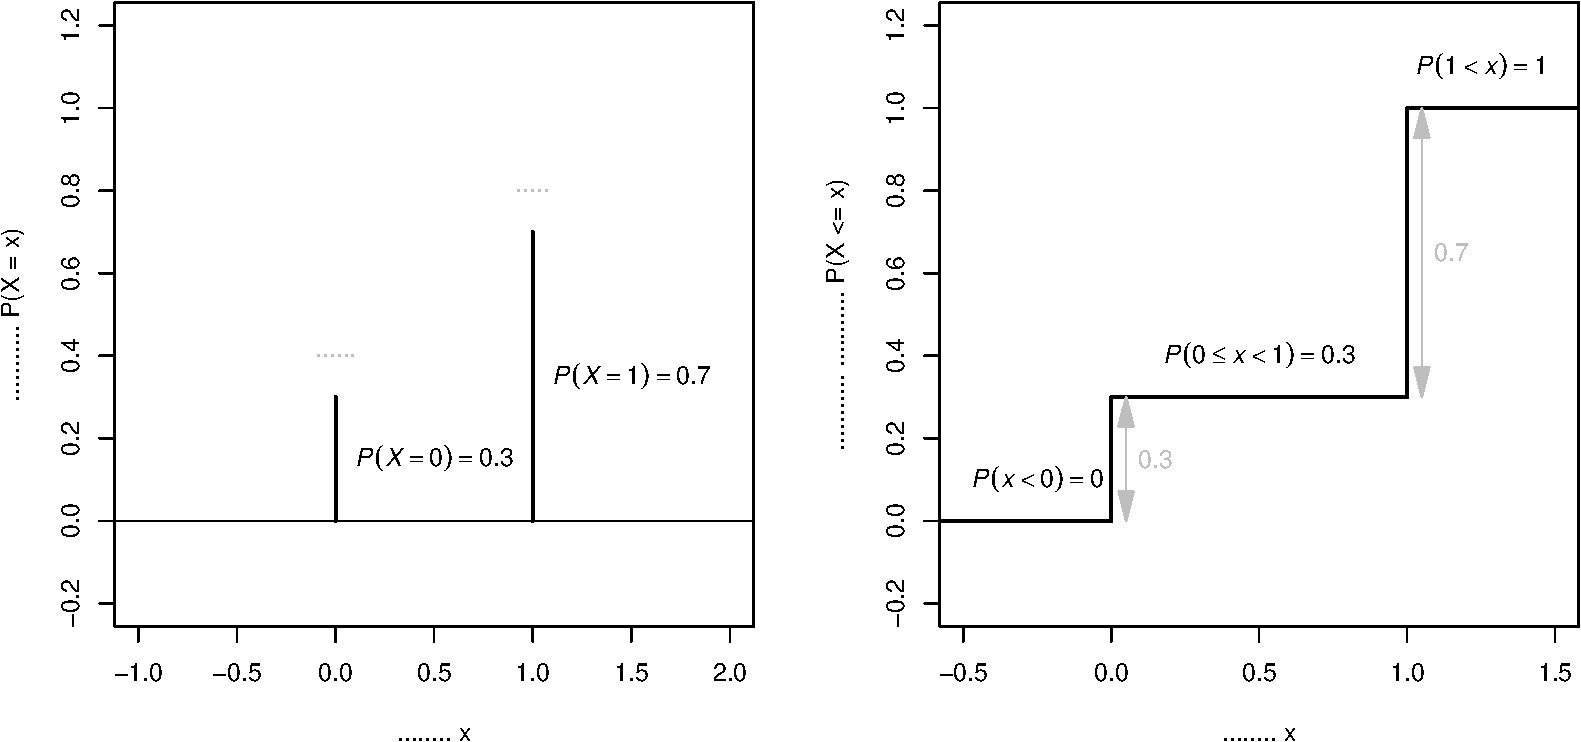
\includegraphics{bookdown-demo_files/figure-latex/fig-3-9-1.pdf}
\caption{\label{fig:fig-3-9}Функція маси ймовірності і функція кумулятивного розподілу для процесу Бернулі із \(p = 0.7\): елементарного підкидання монетки із \(70 \%\) ймовірністю випадіння аверсу.}
\end{figure}

Для дискретних змінних, pmf задана як \(f(x) = P(X = x) \forall x\) і \(P(X = u) = 0\) якщо \(u \notin \mathcal{X}\). Для трансформації pmf в cdf можна обчислити \(F(x) = P(X \leq x) = \sum \limits_{u: u \leq x} P(X = u) = \sum \limits_{u: u \leq x} f(u)\), а для протилежної трансформації cdf в pmf можна обчислити \(f(x) = F(u) - \lim \limits_{h \downarrow 0} F(u - h)\). Для неперервної ж змінної, \(f(u) = F(X = u) - \lim \limits_{h \downarrow 0} F(u - h) = 0\), адже \(P(X = u) = 0 \forall u\); cdf можна перевести в pdf як \(f(x) = \frac{d F(x)}{d x}\), і зворотньо pdf у cdf як \(F(x) = \int \limits_{u: u \leq x} f(u) du\).

Важливим параметром для опису будь-якої функції розподілу ймовірності є \textbf{математичне очікування, або математичне сподівання} (\emph{expectation}). Для всякої функції \(f(x)\), математичне очікування можна знайти як середнє усіх можливих значень \(x: x \in \mathcal{X}\) зважене за ймовірністю цих значень \(f(x)\): відтак, для дискретних розподілів \(X\) математичне очікування змінної оцінюється як \(\mathbb{E}[X] = \sum \limits_{x \in \mathcal{X}} x f(x)\), а для неперервних -- як \(\mathbb{E}[X] = \int \limits_{x \in \mathcal{X}} x f(x) dx\). Подібно до очікування змінної, можна шукати й очікування функції змінної \(g(x)\): \(\mathbb{E}[g(X)] = \sum \limits_{x \in \mathcal{X}} g(x) f(x)\) або \(\mathbb{E}[g(X)] = \int \limits_{x \in \mathcal{X}} g(x) f(x) dx\). Якщо очікування існує (є такі функції, для яких неможливо аналітично вирішити суми чи інтеграли), воно матиме наступні властивості:

\begin{itemize}
\item
  якщо \(c\) константа, то \(\mathbb{E}[c] = c\),
\item
  якщо \(c\) константа і \(g()\) -- функція, то \(\mathbb{E}[c g(X)] = c \mathbb{E} [g(X)]\),
\item
  якщо \(c_1\) та \(c_2\) є константами і \(g_1()\), \(g_2()\) -- функціями, то \(\mathbb{E}[c_1 g_1 (X) + c_2 g_2(X)] = c_1 \mathbb{E}[g_1(X)] + c_2 \mathbb{E}[g_2(X)]\).
\end{itemize}

Математичне очікування змінної \(\mathbb{E}[X]\) ще часто називають \textbf{середнім} (не плутати із середнім арифметичним, яке є середнім для нормального розподілу і деяких інших розподілів). Іншим важливим окремим випадком математичного очікування функції розподілу її ймовірності є її \textbf{варіація} \(Var[X]\) -- очікування середньоквадратичного відхилення випадкової змінної від її середнього:

\[
\begin{aligned}
  Var[X] = \mathbb{E} \left[ (X - \mathbb{E}[X])^2 \right] = \mathbb{E} \left[ X^2 - 2X \mathbb{E} [X] + (\mathbb{E} [X])^2 \right] = \\
  \mathbb{E} [X^2] - 2 \mathbb{E}[X] \mathbb{E}[X] + (\mathbb{E}[X])^2 = \mathbb{E} [X^2] - 2 \mathbb{E}[X] \mathbb{E}[X] + \mathbb{E}[X] \mathbb{E}[X] = \\
  \mathbb{E}[X^2] - \mathbb{E}[X] \mathbb{E}[X] = \mathbb{E}[X^2] - (\mathbb{E}[X])^2
\end{aligned}
\]

Функції розподілу ймовірності можуть приймати будь-який вигляд\footnote{особливо pdf: часто значення функції перевищує одиницю, що викликає справедливе питання ``а як ймовірність може бути більша за одиницю?''. Не може, але й ця функція не повертає ймовірність. Її \emph{інтеграл} повертає ймовірність.}. Розгляньмо окремі випадки поширених розподілів ймовірності. В усіх випадках ми кажемо що випадкова змінна \(X\) походить із певного розподілу \(f(x)\) позначенням \(X \sim \mathcal{A}(\theta, \cdots)\) де \(\theta\) є параметром розподілу \(\mathcal{A}\).

Нижче наведено формули розподілів ймовірності і, якщо доцільно, кумулятивних розподілів для окремих поширених статистичних розподілів. Також наведено значення середнього та варіації цих розподілів з точки зору параметрів і наявні шляхи обчислення \emph{оцінки} параметрів (позначені як \(\hat{\theta}\) для параметру \(\theta\)) для вибірки \(x_i \in X\) розміром \(n\) \footnote{варто зауважити, що формули оцінщиків взяті із відкритих джерел, включно із постами блогів. Кожен розподіл має своєрідну ситуацію із оцінщиками, і виведення оцінщиків не завжди проводиться методом максимальної правдоподібності чи за допомогою момент-генеруючих функцій (ми не торкаємось цього методу), ба того, такі оцінщики іноді є упередженими (biased). Використовувати оцінщики параметрів необхідно із застереженнями!}.

\subsubsection{Дискретні розподіли}\label{ux434ux438ux441ux43aux440ux435ux442ux43dux456-ux440ux43eux437ux43fux43eux434ux456ux43bux438}

\paragraph{Розподіл Бернулі}\label{ux440ux43eux437ux43fux43eux434ux456ux43b-ux431ux435ux440ux43dux443ux43bux456}

Розподіл Бернулі описує дискретну змінну із лише двома класами, відтак, яку можна представити як бінарну змінну: \(x \in \mathcal{X}: \mathcal{X} = \{0, 1\}\). Прикладом слугує підкидання монетки.

\begin{itemize}
\item
  Позначення: \(X \sim \mathcal{Bernoulli}(p)\)
\item
  pmf: \(f(x) = P(X = x) = p^x (1-p)^{x-1}\),
\item
  cdf: \(F(x) = P(X \leq x) = 0 \mathbb{I}_x(x < 0)\), \(P(X \leq x) = (1 - p) \mathbb{I}_x(0 \leq x < 1)\), \(P(X \leq x) = 1 \mathbb{I}_x(1 < x)\).
\item
  середнє \(\mathbb{E} [X] = \frac{N+1}{2} = p\),
\item
  варіація \(Var[X] = p(1 - p)\),
\item
  оцінщик \(\hat{p} = \frac{1}{n} \sum \limits_{i=1}^{n}x_i\).
\end{itemize}

\paragraph{Дискретний рівномірний розподіл}\label{ux434ux438ux441ux43aux440ux435ux442ux43dux438ux439-ux440ux456ux432ux43dux43eux43cux456ux440ux43dux438ux439-ux440ux43eux437ux43fux43eux434ux456ux43b}

Дискретний рівномірний розподіл описує ситуацію, в якій кожна із дискретних величин (\(\mathcal{X} = \{1, 2, 3, \cdots, N\}\)) має однакову ймовірність потрапити у вибірку. Прикладом можуть слугувати гральні кісточки.

\begin{itemize}
\item
  Позначення: \(X \sim \mathcal{DU}(N)\) або \(X \sim \mathcal{DU}(a, b)\) де \(N = b - a + 1 \text { } \forall b \geq a\),
\item
  pmf: \(f(x) = P(X = x) = \frac{1}{N} \mathbb{I}_x (x \in \{0, 1, 2, 3, \cdots, N\})\),
\item
  cdf: \(F(x) = P(X \leq x) = \frac{x - a + 1}{N}\),
\item
  середнє \(\mathbb{E} [X] = \frac{N+1}{2} = \frac{a+b}{2}\),
\item
  варіація \(Var[X] = \frac{N^2 - 1}{12}\),
\item
  оцінщик \(\hat{N} = \frac{n+1}{n} \max (x_i)\).
\end{itemize}

\paragraph{Біноміальний розподіл}\label{ux431ux456ux43dux43eux43cux456ux430ux43bux44cux43dux438ux439-ux440ux43eux437ux43fux43eux434ux456ux43b}

Проведіть \(n\) незалежних випадкових експериментів Бернулі: \(X \sim \mathcal{Bernoulli}(p)\). Якщо позначити \(y\) як кількість успішних експериментів в \(X\) із \(n\) спроб, то \(Y\) описуватиметься біноміальним розподілом.

\begin{itemize}
\item
  Позначення: \(Y \sim \mathcal{Binomial}(n, p)\),
\item
  pmf: \(f(Y) = P(Y = y) = \binom{n}{y} p^y (1-p)^{n - y} \mathbb{I}_y (y \in \{0, 1, 2, \cdots, n\})\)\footnote{cdf біноміального розподілу існує, але його складно вивести і він все одно мало що скаже; варіацію біноміального розподілу також шукати відносно непросто.},
\item
  середнє \(\mathbb{E} [Y] = np\) \footnote{обчислення очікування із біноміальними коефіцієнтами включає розкладання біному: \((a + b)^n = \sum \limits_{x = 0}^n \binom{n}{x} a^x b^{n - x}\)},
\item
  варіація \(Var[Y] = np(1-p)\),
\item
  оцінщик \(\hat{p} = \frac{y}{n}\).
\end{itemize}

\paragraph{Геометричний розподіл}\label{ux433ux435ux43eux43cux435ux442ux440ux438ux447ux43dux438ux439-ux440ux43eux437ux43fux43eux434ux456ux43b}

Уявіть повторення випадкового експерименту Бернулі із параметром \(p\) до того, поки не випаде перший успіх. В такому випадку, можна розрахувати кількість безуспішних спроб \(x\) до першого успіху та кількість спроб \(y\) потрібних для першого успіху. Обидві змінні описуються геометричним розподілом.

\begin{itemize}
\tightlist
\item
  pmf:
\end{itemize}

\[f(x) = P(X = x) = p(1 - p)^x \mathbb{I}_x (0, 1, 2, \cdots, \infty)\]

\[f(y) = P(Y = y) = p(1-p)^{y-1} \mathbb{I}_y (0, 1, 2, \cdots, \infty)\]

\begin{itemize}
\tightlist
\item
  середні
\end{itemize}

\[\mathbb{E} [X] = \frac{1-p}{p}\]

\[\mathbb{E} [Y] = \frac{1}{p}\]

\begin{itemize}
\tightlist
\item
  варіації
\end{itemize}

\[Var[X] = \frac{1-p}{p^2}\]

\[Var[Y] = \frac{1-p}{p^2}\]

\begin{itemize}
\tightlist
\item
  оцінщик \(\hat{p} = \frac{1}{x}\).
\end{itemize}

\paragraph{Негативний біноміальний розподіл}\label{ux43dux435ux433ux430ux442ux438ux432ux43dux438ux439-ux431ux456ux43dux43eux43cux456ux430ux43bux44cux43dux438ux439-ux440ux43eux437ux43fux43eux434ux456ux43b}

Негативний біноміальний розподіл описує \(X\) як кількість невдач перед \(r\)-тим успіхом в серії випадкових експериментів Бернулі із параметром \(p\).

\begin{itemize}
\item
  Позначення: \(X \sim \mathcal{NBinom} (r, p)\),
\item
  pmf: \(f(x) = P(X = x) = \binom{\text{спроби}}{\text{успіхи} + x \text{ невдач}} \cdot \text{невдачі} \cdot \text{успіхи} = \binom{x + r - 1}{r-1} (1-p) ^x p^r\),
\item
  середнє \(\mathbb{E} [X] = \frac{r(1-p)}{p}\),
\item
  варіація \(Var[X] = \frac{r(1-p)}{p^2}\),
\item
  оцінщик \(\hat{p} = \frac{r-1}{r + x - 1}\).
\end{itemize}

Примітно, що геометричний розподіл є окремим випадком негативного біноміального розподілу. Якщо \(Y\) -- кількість спроб для отримання \(r\) успіхів, то \(Y = X + r\), \(P(Y = y) = \binom{y-1}{r-1} (1-p)^{y-r} p^r\). \(\mathbb{E}[Y] = \mathbb{E}[X] + r\), \(Var[Y] = Var[X]\).

\paragraph{Розподіл Пуасона}\label{ux440ux43eux437ux43fux43eux434ux456ux43b-ux43fux443ux430ux441ux43eux43dux430}

Мабуть, один із найменш інтуїтивно зрозумілих але найбільш поширених розподілів. Він описує кількість подій, які відбуваються протягом визначеного вікна в просторі, при тому що всі події є незалежними один від одного. Існує чимало прикладів процесів Пуасона, наприклад, кількість людей на платформі залізничної станції в момент часу чи кількість особин популяції зареєстрованих на ділянці.

\begin{itemize}
\item
  Позначення: \(X \sim \mathcal{Poisson}(\lambda)\)
\item
  pmf: \(f(x) = P(X = x) = e^{-\lambda} \frac{\lambda^x}{x!}\), де \(x \in \{0, 1, 2, 3, \cdots, \infty \}\), \(\lambda > 0\),
\item
  середнє \(\mathbb{E} [X] = \lambda\),
\item
  варіація \(Var[X] = \lambda\),
\item
  оцінщик \(\hat{\lambda} = \frac{1}{n} \sum \limits_{i=1}^{n}x_i\).
\end{itemize}

Цікаво, що \(Y \sim \mathcal{Binomial}(n, p)\) із не-екстремальним значенням \((np)\) та дуже значним \(n\) може бути апроксимована до розподілу Пуасона із \(\lambda \approx np\).

\paragraph{Гіпергеометричний розподіл}\label{ux433ux456ux43fux435ux440ux433ux435ux43eux43cux435ux442ux440ux438ux447ux43dux438ux439-ux440ux43eux437ux43fux43eux434ux456ux43b}

Уявіть зліченну популяцію розміром \(N\) із об'єктів, що належать до різних класів, зокрема, в якій існує \(K: K \leq N\) об'єктів із певною характеристикою (наприклад, особини виду, в якому ми зацікавлені, в угрупованні різних видів\footnote{застосування гіпергеометричного розподілу в реальних задачах екології угруповань може бути складним, адже чисельності видів можуть сягати сотень і тисяч, й обчислення біноміальних коефіцієнтів видасть дуже великі числа -- іноді настільки великі, що комп'ютер не може їх обчислити і зве безкінечністю. Аби обійти обмеження стандартної комп'ютерної архітектури в нагоді можуть стати функції із бібліотеки \texttt{gmp} для R.}). Тоді можна очікувати, що вибірка розміром \(n\) із цілої популяції міститиме \(x\) об'єктів із шуканого класу.

\begin{itemize}
\item
  Позначення: \(X \sim \mathcal{HyperGeom}(N, K, n)\),
\item
  pmf: \(f(x) = P(X = x) = \frac{\binom{N}{K} \binom{N-K}{n - x}}{\binom{N}{n}}\),
\item
  середнє \(\mathbb{E} [X] = n \frac{K}{N}\),
\item
  оцінщик для \href{https://math.stackexchange.com/questions/40319/maximum-likelihood-estimate-of-hypergeometric-distribution-parameter}{випадків апроксимації до розподілу Пуасона} де \(K/N << 1, n >> 1\): \(\hat{m} = \frac{N \sum \limits_i^T x_i}{Tn}\) для вибірки \(x_i \in X\) розміром \(T\).
\end{itemize}

\paragraph{Нуль-упереджені моделі}\label{ux43dux443ux43bux44c-ux443ux43fux435ux440ux435ux434ux436ux435ux43dux456-ux43cux43eux434ux435ux43bux456}

Доволі цікавою родиною розподілів, котрі часто застосовують в екологічних дослідженнях, є ``нуль-упереджені'', або ``нуль-надуті'' моделі (zero-inflated models). Такі моделі описують розподіли, в котрих значна частка спостережених значень припадає на нулі. Такі розподіли можуть описувати спостережені чисельності виду у вибірці спостережень якщо, зазвичай, ми не спостерігаємо вид (відповідно, чисельність дорівнює нулю), але якщо спостерігаємо, то чисельність відповідає якомусь позитивному цілому значенню. Відтак, якщо ігнорувати всі нульові спостереження, то чисельність описуватиметься якимось симпатичним дискретним розподілом, однак, нульові спостереження не можна просто так ігнорувати.

Насправді, нуль-упереджені моделі є комбінацією двох розподілів: один генерує нулі, в той час як інший генерує позитивні дискретні значення. Найбільш поширеним розподілом в цій родині є нуль-упереджений розподіл Пуасона (zero-inflated Poisson, ZIP): нуль-генеруюча частина цього процесу визначає чи випадкове значення дорівнюватиме нулю, і якщо ні, тоді випадкове значення отримується із звичайного розподілу Пуасона (який також може генерувати нулі, але набагато менше). Відтак, ZIP матиме два параметри: (1) ймовірність того, що нуль-генеруюча функція поверне нуль (\(p\)), та (2) параметр розподілу Пуасона (\(\lambda\)). Математично, такий розподіл можна визначити як \(X \sim \mathcal{ZIP}(p, \lambda)\)

\[
P(X = x_i) = 
\begin{cases}
P(X = 0) = p + (1-p)e^{-\lambda}\\
P(X = x_i) = (1 - p) \frac{\lambda^{x_i} e^{-\lambda}}{x_i!} \text{ } \forall \text{ } x_i = \{1, 2, 3, \cdots\}
\end{cases}
\]

\begin{itemize}
\item
  середнє \(\mathbb{E} [X] = (1-p) \lambda\),
\item
  варіація \(Var[X] = (1-p)\lambda \cdot (1+p \lambda)\),
\item
  оцінщики \(\hat{\lambda} = \frac{s^2 + \bar{x}^2}{\bar{x}} - 1\), \(\hat{p} = \frac{s^2 - \bar{x}}{s^2 + \bar{x}^2 - \bar{x}}\) де \(\bar{x} = \frac{1}{n} \sum x_i\), \(s^2 = \frac{1}{n - 1} \sum (x_i - \bar{x})^2\).
\end{itemize}

\subsubsection{Континуальні розподіли}\label{ux43aux43eux43dux442ux438ux43dux443ux430ux43bux44cux43dux456-ux440ux43eux437ux43fux43eux434ux456ux43bux438}

\paragraph{Рівномірний розподіл}\label{ux440ux456ux432ux43dux43eux43cux456ux440ux43dux438ux439-ux440ux43eux437ux43fux43eux434ux456ux43b}

Рівномірний розподіл описує ситуацію, коли будь-яке значення \(x\) між \(a\) і \(b\) має рівну ймовірність: \(P(a \leq X \leq b) = 1\).

\begin{itemize}
\item
  Позначення: \(X \sim \mathcal{U}(a, b)\),
\item
  pdf: \(f(x) = \frac{1}{b-a} \mathbb{I}_x (a \leq x \leq b)\) (примітно, що функція є константою),
\item
  cdf: \(F(x) = P(X \leq x) = \frac{x-a}{b-a} \text { } \forall (a \leq x \leq b)\), але \(F(X) = 0 \mathbb{I}_x(x < 0)\) і \(F(X) = 1 \mathbb{I}_x (1 < x)\),
\item
  середнє \(\mathbb{E} [X] = \frac{a+b}{2}\),
\item
  варіація \(Var[X] = \frac{(b-a)^2}{12}\),
\item
  оцінщики \(\hat{a} = \min(x_i), \hat{b} = \max(x_i)\).
\end{itemize}

\paragraph{Бета-розподіл}\label{ux431ux435ux442ux430-ux440ux43eux437ux43fux43eux434ux456ux43b}

Доволі різноманітна родина розподілів із формою функції, яка контролюється двома параметрами, \(a\) і \(b\). Щодо цього розподілу, мабуть, варто просто знати про його існування. Його іноді застосовують в популяційній генетиці \href{https://doi.org/10.1007\%2FBF01441146}{(Balding \& Nichols 1995)} та Баєсівському аналізі \href{https://doi.org/10.1109/MFI.2016.7849531}{(Jøsang 2016)}.

\begin{itemize}
\item
  Позначення: \(X \sim \mathcal{Beta}(a, b)\),
\item
  pdf: \(f(x) \propto x^{a - 1} (1-x)^{b-1} \mathbb{I}_x(0 < x < 1)\), \(f(x) = \frac{\Gamma (a + b)}{\Gamma (a) \Gamma (b)} x^{a - 1} (1 - x)^{b - 1}\), де \(\Gamma()\) - гамма-функція \(\Gamma(\alpha) = \int \limits_0^{\infty} u^{\alpha - 1} e^{-u} du\).
\item
  середнє \(\mathbb{E} [X] = \frac{a}{a + b}\),
\item
  варіація \(Var[X] = \frac{ab}{(a+b)^2 (a+b+1)}\).
\end{itemize}

\paragraph{Експоненційний розподіл}\label{ux435ux43aux441ux43fux43eux43dux435ux43dux446ux456ux439ux43dux438ux439-ux440ux43eux437ux43fux43eux434ux456ux43b}

Експоненційний розподіл є своєрідним неперервним аналогом геометричного розподілу і описує відстань між незалежними неперервними подіями, які відбуваються із постійним темпом. Розподіл темпів смертності в природних популяціях нагадує експоненційний \href{https://doi.org/10.1016/0022-5193(79)90098-5}{(Abernethy 1979)}.

\begin{itemize}
\item
  Позначення: \(X \sim \mathcal{Exp}(\lambda)\),
\item
  pdf: \(f(x) = \frac{1}{\lambda} e^{-\frac{x}{\lambda}} \mathbb{I}_x (0 \leq x \leq \infty)\),
\item
  cdf: \(F(x) = 1 - e^{-\frac{x}{\lambda}}\),
\item
  середнє \(\mathbb{E} [X] = \lambda\),
\item
  варіація \(Var[X] = \lambda^2\),
\item
  оцінщик \(\hat{(\frac{1}{\lambda})} = \frac{1}{n} \sum x_i\) із упередженням, або \(\hat{(\frac{1}{\lambda})} = \frac{n-2}{\sum x_i}\).
\end{itemize}

Цікавою властивістю експоненційного процесу є відсутність пам'яті: ймовірність вижити в наступний момент часу за умови виживання до цього моменту дорівнює ймовірності вижити в будь-який момент часу (\(P(X > (s+t)|X > s) = P(X > t)\)).

Особливим випадком експоненційного розподілу є двопараметричний \textbf{зміщений експоненційний розподіл}: \(f(x) = \frac{1}{\lambda} e^{-\frac{x - \mu}{\lambda}} \mathbb{I}_x (\mu \leq x \leq \infty)\), для якого середнє дорівнює \(\mathbb{E}[X] = \mu + \lambda\).

\paragraph{Нормальний розподіл}\label{ux43dux43eux440ux43cux430ux43bux44cux43dux438ux439-ux440ux43eux437ux43fux43eux434ux456ux43b}

Мабуть, найбільш знаменитий розподіл, яким можна описати чимало змінних в біології: розміри листків рослин, зріст людей певного віку тощо. Його логіка доволі проста і каже що змінна \(X\) матиме значення \(x\), які концентруються навколо якогось середнього значення \(\bar{x}\), і чим сильніше \(x\) відрізняються від \(\bar{x}\), тим менш поширеними вони будуть. Цьому розподілу варто приділити дещо більше уваги, аніж іншим.

\begin{itemize}
\item
  Позначення: \(X \sim \mathcal{N}(\mu, \sigma^2)\), де параметр \(\mu: \{-\infty \leq \mu \leq \infty\}\) відповідає середньому значенню (а також \textbf{\emph{медіані}} \footnote{\textbf{медіана} -- значення в сортованій послідовності випадкової змінної \(X\), яке розділяє цю послідовність на дві частини однакового розміру; медіана тісно пов'язана із поняттями \textbf{перцентилів} \(x_{\alpha}\) -- такими значеннями \(x\), які більше за частку \(\alpha\) випадкової змінної \(X\) (наприклад, перцентиль \(x_{\alpha = 0.95}\) -- це таке значення, що в змінній \(X\) \(95 \%\) значень менше або дорівнюють \(x_{\alpha = 0.95}\)). Медіана відповідає перцентилю із \(\alpha = 0.5\).} та \textbf{\emph{моді}} \footnote{\textbf{мода} -- найбільш поширене значення у вибірці.}), а параметр \(\sigma^2: \sigma > 0\) відповідає варіації в розподілі, що виражається в ширині характерної куполоподібної кривої.
\item
  pdf: \(f(x) = \frac{1}{\sqrt{2 \pi} \sigma} e^{-\left[ \frac{(x - \mu)^2}{2 \sigma^2} \right]}\),
\item
  середнє \(\mathbb{E} [X] = \mu\),
\item
  варіація \(Var[X] = \sigma^2\).
\end{itemize}

Хорошою демонстрацією методу \hyperref[mle]{максимальної правдоподібності} є пошук параметрів із такої вибірки \(X\) що \(X \sim \mathcal{N}(\mu, \sigma^2)\). Знайдемо функцію правдоподібності:

\[\mathcal{L}(X | \mu, \sigma^2) = \prod \limits_{i=1}^n f(x_i| \mu, \sigma^2) = \prod \limits_{i=1}^n \frac{1}{\sqrt{2 \pi} \sigma} e^{-\left[ \frac{(x - \mu)^2}{2 \sigma^2} \right]} = \left( \frac{1}{\sqrt{2 \pi \sigma^2}} \right)^n \exp \left[ - \frac{\sum \limits_{i=1}^n (x_i - \mu)}{2 \sigma^2} \right]\]

Оскільки бавитись з такою формулою виглядає тією ще задачею, візьмемо логарифм правдоподібності:

\[\ln \mathcal{L}(X | \mu, \sigma^2) = - \frac{n}{2} \ln{(2 \pi \sigma^2)} - \frac{\sum \limits_{i=1}^n (x_i - \mu)}{2 \sigma^2}\]

Знайдемо оцінщик \(\hat{\mu}\) першим. Для цього потрібно продиференціювати попередній вираз відносно \(\mu\) і прирівняти його до нуля:

\[\frac{\partial \ln \mathcal{L}(X | \mu, \sigma^2)}{\partial \mu} = \frac{\sum \limits_{i=1}^n (x_i - \mu)}{\sigma^2} = 0\]
Відтак, рішення

\[\sum \limits_{i=1}^n (x_i - \mu) = 0 \Rightarrow \sum \limits_{i=1}^n x_i - n \mu = 0 \Rightarrow \hat{\mu} = \frac{\sum \limits_{i=1}^n x_i}{n}\]
Що ніщо інше як середнє арифметичне. Щодо іншого параметру, \(\sigma^2\),

\[\frac{\partial \ln \mathcal{L}(X | \mu, \sigma^2)}{\partial \sigma^2} = - \frac{n}{2} \cdot \frac{2 \pi}{2 \pi \sigma^2} + \frac{\sum \limits_{i=1}^n (x_i - \mu)^2}{2 (\sigma^2)^2} = 0 \Rightarrow -n \sigma^2 + \sum \limits_{i=1}^n (x_i - \mu)^2 = 0\]

Можна підставити \(\hat{\mu} = \frac{1}{n} \sum \limits_{i=1}^n x_i = \bar{x}\) і отримати

\[\hat{\sigma^2} = \frac{1}{n} \sum \limits_{i=1}^n (x_i - \bar{x})^2\]

Якщо читач дещо обізнаний в базовій статистиці, то можна помітити що цією формулою \emph{не} користуються для оцінки дисперсії у вибірках із нормального розподілу. Все через те, що такий оцінщик не проходить перевірку на упередженість (bias: оцінщик вважається неупередженим якщо \(\mathbb{E}[\hat{\theta}] = \theta\)): якщо переформулювати (подано без покрокових обчислень, можна перевірити якщо пам'ятати що \(\frac{1}{n} \sum \limits_{i=1}^n x_i \equiv \bar{x}\))

\[\hat{\sigma^2} = \frac{1}{n} \sum \limits_{i=1}^n (x_i - \bar{x})^2 = \frac{1}{n} \sum \limits_{i=1}^n x_i^2 - (\bar{x})^2\]

Тоді (пам'ятаючи що \(\sigma^2 = Var[X] = \mathbb{E} [X^2] - (\mathbb{E} [X])^2 = \mathbb{E} [X^2] - \mu^2\))

\[
\begin{aligned}
  \mathbb{E} [\hat{\sigma^2}] = \mathbb{E} \left[ \frac{1}{n} \sum \limits_{i=1}^n x_i^2 - (\bar{x})^2 \right] = \frac{1}{n} \sum \limits_{i = 1}^n \mathbb{E} [x_i^2] - \mathbb{E} [\bar{x}^2] = \\
  \frac{1}{n}  \sum \limits_{i = 1}^n (\sigma^2 + \mu^2) - (\frac{\sigma^2}{n} + \mu^2) = (1 - \frac{1}{n}) \sigma^2 \neq \sigma^2
\end{aligned}
\]

Натомість, неупередженим оцінщиком \(\hat{\sigma^2}\) є щось, що називають \textbf{дисперсією вибірки}: \(\hat{\sigma^2} = s^2 = \frac{1}{n-1} \sum \limits_{i=1}^n (x_i - \bar{x})^2\). Аби уникнути термінологічної плутанини (а вона чомусь завжди наявна в оцінках варіації), варто визначити наступні дескриптори варіації, що часто застосовуються до вибірок із нормальним розподілом (використовуйте тест Шапіро-Вілка (Shapiro-Wilk test) для перевірки нормальності вибірки; \(p > 0.05\), на відміну від більшості статистичних тестів, є підставою вважати вибірку нормально розподіленою):

\begin{itemize}
\item
  \textbf{\emph{дисперсія}} (\emph{sample variance}) є неупередженим оцінщиком параметру нормального розподілу у вибірці: \(s^2 = \frac{1}{n-1} \sum \limits_{i=1}^n (x_i - \bar{x})^2\), якому в R відповідає функція \texttt{var()},
\item
  \textbf{\emph{середньоквадратичне відхилення}} описує варіацію вибірки незалежно від її розподілу: \(v^2 = \frac{1}{n} \sum \limits_{i=1}^n (x_i - \bar{x})^2\); однак набагато частіше під цим терміном (як і будемо ми) розуміють кориговане \textbf{\emph{стандартне відхилення}} (\emph{standard deviation}, SD): \(s = \sqrt{\frac{1}{n-1} \sum \limits_{i=1}^n (x_i - \bar{x})^2}\), якому в R відповідає функція \texttt{sd()},
\item
  \textbf{\emph{стандартна помилка}} (\emph{standard error}, SE) описує відхилення вибіркового середнього \(\bar{x}\): \(\frac{s}{\sqrt{n}}\).
\end{itemize}

Щодо важливості нормального розподілу в статистиці, варто згадати закон великих чисел та центральну граничну теорему. \textbf{Закон великих чисел} стверджує, що якщо із \textbf{\emph{генеральної сукупності}} \footnote{\textbf{генеральна сукупність} -- поширене поняття в статистиці; якщо спостерігач обрав вибірку значень (наприклад, вага особин модельного виду), ця вибірка є лише обмеженою підмножиною генеральної сукупності, розмір якої апроксимує до безкінечності. Ми припускаємо що вибірка є репрезентативною щодо генеральної сукупності, отже, розподіл ймовірності в генеральній сукупності апроксимує до розподілу в генеральній сукупності. Неможливо набрати вибірку розміром із розмір генеральної сукупності -- спостерігач завжди пропустить бодай один зразок.} незалежно і багаторазово набирати окремі вибірки, то усереднена статистика\footnote{статистика -- інше слово для параметру вибірки або параметру тесту. Середнє арифметичне є статистикою, дисперсія є статистикою тощо.} цих вибірок наближається до істинного значення статистики генеральної сукупності, якщо таке існує. В контексті нормального розподілу, середні вибірок (\(\hat{\mu}\)) з генеральної сукупності конвергують до середнього генеральної сукупності \(\mu\). \textbf{Центральна гранична теорема} ж постулює, що в множині таких незалежних \emph{змінних} \(X_1, X_2, X_3, \cdots, X_n\), що \(\mathbb{E} [X_i] = \mu\), \(Var[X_i] = \sigma^2\), незалежно від розподілу окремих змінних \(X_i\), за \(n \rightarrow \infty\) розподіл змінних \(\sqrt{n} (\frac{1}{n}\sum \limits_{i=1}^n X_i - \mu)\) конвергує до \(\mathcal{N}(0,  \sigma^2)\). Іншими словами, яким би не був розподіл генеральної сукупності, розподіл середніх значень вибірок із такої генеральної сукупності буде нагадувати нормальний розподіл.

Корисною технікою є \textbf{z-стандартизація} (\emph{z-scaling}), за допомогою якої будь-яку вибірку можна трансформувати в таку, в якої \(\mu = 0, \sigma^2 = 1\) (припускаючи, що вибірка розподілена нормально, але техніка працює для будь-якого розподілу): \(z_i = \frac{x_i - \bar{x}}{s}\). Такий нормальний розподіл, що \(\mathcal{N} (\mu = 0, \sigma^2 = 1)\) називається \textbf{cтандартним нормальним розподілом}.

\paragraph{Лог-нормальний розподіл}\label{ux43bux43eux433-ux43dux43eux440ux43cux430ux43bux44cux43dux438ux439-ux440ux43eux437ux43fux43eux434ux456ux43b}

Змінна \(X\) розподілена лог-нормально (\(X \sim L\mathcal{N}(\mu, \sigma^2)\)) якщо \(\ln(X) \sim \mathcal{N}(\mu, \sigma^2)\). Відтак, якщо поглянути з іншого боку, то якщо \(Y \sim \mathcal{N}(\mu, \sigma^2)\), то \(X = e^Y \sim L\mathcal{N}(\mu, \sigma^2)\).

\begin{itemize}
\item
  Середнє \(\mathbb{E} [\ln (X)] = \mu, \mathbb{E}[X] = e^{\mu + \frac{\sigma^2}{2}}\),
\item
  варіація \(Var[\ln(X)] = \sigma^2, Var[X] = \exp [2(\mu - \sigma^2)] - \exp [2 \mu + \sigma^2]\).
\end{itemize}

\paragraph{Розподіл Коші}\label{ux440ux43eux437ux43fux43eux434ux456ux43b-ux43aux43eux448ux456}

Доволі дивний розподіл, який формою нагадує нормальний із набагато гострішим піком та товстішими хвостами.

\begin{itemize}
\item
  Позначення: \(X \sim \mathcal{Cauchy}(x_0, \gamma)\), де \(\gamma\) регулює форму кривої, а \(x_0\) відповідає локації піку.
\item
  pdf: \(f(x) = \frac{1}{\pi} \left[ \frac{\gamma}{(x - x_0)^2 + \gamma^2} \right]\)
\end{itemize}

Дивність цього розподілу полягає в тому, що його середнє й варіація неможливо аналітично визначити. Оцінки середнього арифметичного і cередньоквадратичного відхилення не конвергують зі збільшенням розміру вибірки, а єдиним більш-менш точним методом оцінки параметру форми \(\hat{\gamma}\) є медіана абсолютних значень вибірки.

\subsection{Опис розподілу змінної (описова статистика)}\label{bars}

Уявімо вибірку змінної \(X \sim \mathcal{N}(\mu = 15, \sigma^2 = 9)\) розміром \(n = 1000\):

\begin{Shaded}
\begin{Highlighting}[]
\CommentTok{\# визначимо рандомне зерно для повторюваності коду}
\FunctionTok{set.seed}\NormalTok{(}\DecValTok{1234}\NormalTok{)}

\CommentTok{\# визначимо змінну як випадкову вибірку із нормального розподілу із визначеними параметрами}
\NormalTok{X }\OtherTok{\textless{}{-}} \FunctionTok{rnorm}\NormalTok{(}\AttributeTok{n =} \DecValTok{1000}\NormalTok{, }\AttributeTok{mean =} \DecValTok{15}\NormalTok{, }\AttributeTok{sd =} \FunctionTok{sqrt}\NormalTok{(}\DecValTok{9}\NormalTok{))}
\end{Highlighting}
\end{Shaded}

Як описати тенденції цієї вибірки одним-двома параметрами? Мабуть, більшість автоматично скажуть ``давайте порахуємо середнє'', хтось додасть ``і варіацію у вигляді середньоквадратичного відхилення чи дисперсії''. Натомість, навіть на цьому етапі вирішення статистики для опису змінної варто задати собі питання: а що нам ці статистики дадуть? По-перше, як мінімум, ми хочемо отримати такі значимі і продумані статистики, із якими, якщо потрібно, можна спробувати відтворити вибірку. По-друге, як ми побачили в попередньому підрозділі, існує чимало розподілів ймовірності, і \emph{найгірше, що можна зробити -- це спробувати описати змінну із певним розподілом параметром не цього розподілу} (наприклад, намагатись оцінити параметри \(a\) і \(b\) бета-розподілу, коли вибірка відповідає Пуасонівському процесу). Дуже важливим неписаним правилом статистичного аналізу є те, що \textbf{в більшості випадків оцінщик чи статистичний тест видасть якийсь результат для даних, які в нього введені, і, може, навіть видасть якесь значення \(p\) (див. \hyperref[pval]{нижче}), але цей результат нічого не значить якщо обрано некоректну статистичну процедуру для певного набору даних}. Крім того, завжди мати на увазі принцип \textbf{``garbage in, garbage out''} (``сміття на вході, сміття на виході''): навіть якщо логіка статистичного аналізу правильна і програма функціонує коректно, результати не можна вважати валідними якщо вхідні дані помилкові.

Це дуже довгий спосіб сказати, що для вибору метрики центральної тенденції у вибірці варто враховувати розподіл цієї вибірки. Не можна розраховувати, скажімо, середнє арифметичне просто тому, що так зручно. Натомість, вибір статистики повинен бути виважений і відповідати передбаченому розподілу змінної\footnote{наприклад, як розрахувати узагальнену кількість особин виду для повторних спостережень на певній локації? Свого часу мені казали рахувати максимальну кількість особин між спостереженнями, однак такий підхід не є коректним. Натомість, якщо розглядати спостереження особин як біноміальний процес або процес Пуасона, за обох розподілів середнє арифметичене слугує виправданим оцінщиком. Для поглибленого погляду в цю тему, див. \hyperref[detectability]{ймовірність детекції}}. В нашому випадку, ми знаємо що \(X\) згенеровано як нормальний процес, але давайте про всяк випадок перевіримо чи ця змінна дійсно розподілена нормально.

\begin{Shaded}
\begin{Highlighting}[]
\FunctionTok{shapiro.test}\NormalTok{(X)}
\end{Highlighting}
\end{Shaded}

\begin{verbatim}
## 
##  Shapiro-Wilk normality test
## 
## data:  X
## W = 0.99737, p-value = 0.1053
\end{verbatim}

Тест Шапіро-Вілка видає \(p = 0.105 > 0.05\), що у випадку цього тесту дає підстави вважати, що змінна дійсно розподілена нормально. Відтак, центральну тенденцію можна описати середнім арифметичним, адже воно відповідає оцінщику очікування нормального розподілу.

\begin{Shaded}
\begin{Highlighting}[]
\FunctionTok{mean}\NormalTok{(X)}
\end{Highlighting}
\end{Shaded}

\begin{verbatim}
## [1] 14.92021
\end{verbatim}

Які є альтернативи середньому арифметичному? Популярним вибором є \textbf{медіана}, особливо в якості \textbf{\emph{непараметричної статистики}} -- такої статистики, яка вимагає мінімальних передбачень щодо розподілу даних і може бути використана для змінних із будь-яким розподілом. В багатьох випадках змінні в даних матимуть дивний (асиметричний, бімодальний тощо) розподіл. В таких випадках можна спробувати провести тест Шапіро-Вілка, який скоріш за все не підтримає припущення про нормальний розподіл (\(p < 0.05\)). Якщо є припущення про якийсь інший розподіл, його можна перевірити із тестом \textbf{Колмогорова-Смірнова}\footnote{\textbf{Тест Колмогорова-Смірнова} використовують для перевірки гіпотези, що дві вибірки отримані із одного неперервного розподілу. Іншими словами, тестом Колмогорова-Смірнова можна перевірити розподіл змінної (навіть непараметричний розподіл, якщо наявна його адекватна pdf).}. Порівняймо нашу вибірку із нормальним розподілом (хоча ми й так вже знаємо із тесту Шапіро-Вілка відповідь).

\begin{Shaded}
\begin{Highlighting}[]
\CommentTok{\# z{-}стандартизація вибірки потрібна, адже розподіл для порівняння є за замовчуванням стандартним нормальним розподілом}
\NormalTok{Z }\OtherTok{\textless{}{-}} \FunctionTok{scale}\NormalTok{(X)}

\CommentTok{\# порівняймо із ідеальним випадком, для чого наведемо назву функції кумулятивного нормального розподілу}
\FunctionTok{ks.test}\NormalTok{(}\AttributeTok{x =}\NormalTok{ Z, }\AttributeTok{y =} \StringTok{"pnorm"}\NormalTok{)}
\end{Highlighting}
\end{Shaded}

\begin{verbatim}
## 
##  Asymptotic one-sample Kolmogorov-Smirnov test
## 
## data:  Z
## D = 0.021443, p-value = 0.7474
## alternative hypothesis: two-sided
\end{verbatim}

\begin{Shaded}
\begin{Highlighting}[]
\CommentTok{\# альтернативно, можна для порівняння використати іншу випадкову вибірку із нормальним розподілом}
\FunctionTok{ks.test}\NormalTok{(Z, }\FunctionTok{rnorm}\NormalTok{(}\AttributeTok{n =} \FunctionTok{length}\NormalTok{(Z)))}
\end{Highlighting}
\end{Shaded}

\begin{verbatim}
## 
##  Asymptotic two-sample Kolmogorov-Smirnov test
## 
## data:  Z and rnorm(n = length(Z))
## D = 0.026, p-value = 0.8879
## alternative hypothesis: two-sided
\end{verbatim}

\begin{Shaded}
\begin{Highlighting}[]
\CommentTok{\# або порівняти вихідну не{-}стандартизовану змінну із випадковою нормальною вибіркою із середнім та варіацією вихідної вибірки}
\FunctionTok{ks.test}\NormalTok{(X, }\FunctionTok{rnorm}\NormalTok{(}\AttributeTok{n =} \FunctionTok{length}\NormalTok{(X), }\AttributeTok{mean =} \FunctionTok{mean}\NormalTok{(X), }\AttributeTok{sd =} \FunctionTok{sd}\NormalTok{(X)))}
\end{Highlighting}
\end{Shaded}

\begin{verbatim}
## 
##  Asymptotic two-sample Kolmogorov-Smirnov test
## 
## data:  X and rnorm(n = length(X), mean = mean(X), sd = sd(X))
## D = 0.036, p-value = 0.5361
## alternative hypothesis: two-sided
\end{verbatim}

Оскільки вибірка \(X \sim \mathcal{N}()\), можна перебачити що медіана приблизно дорівнюватиме середньому арифметичному, відтак, для нормальних вибірок немає змісту наводити інший параметр окрім середнього.

\begin{Shaded}
\begin{Highlighting}[]
\FunctionTok{mean}\NormalTok{(X)}
\end{Highlighting}
\end{Shaded}

\begin{verbatim}
## [1] 14.92021
\end{verbatim}

\begin{Shaded}
\begin{Highlighting}[]
\FunctionTok{median}\NormalTok{(X)}
\end{Highlighting}
\end{Shaded}

\begin{verbatim}
## [1] 14.88062
\end{verbatim}

Якби ми підходили до непараметричного аналізу вибірки із не-нормальним розподілом, варто було би використовувати лише медіану. Класичним прикладом є уявний експеримент із вибіркою з трьох людей: одним мільйонером (зарплатня \(\$1000000\) на місяць) та двома бідняками (\(\$100\) на місяць). Яка середня зарплатня і яка медіана в такій популяції?

\begin{Shaded}
\begin{Highlighting}[]
\FunctionTok{mean}\NormalTok{(}\FunctionTok{c}\NormalTok{(}\DecValTok{1000000}\NormalTok{, }\DecValTok{100}\NormalTok{, }\DecValTok{100}\NormalTok{))}
\end{Highlighting}
\end{Shaded}

\begin{verbatim}
## [1] 333400
\end{verbatim}

\begin{Shaded}
\begin{Highlighting}[]
\FunctionTok{median}\NormalTok{(}\FunctionTok{c}\NormalTok{(}\DecValTok{1000000}\NormalTok{, }\DecValTok{100}\NormalTok{, }\DecValTok{100}\NormalTok{))}
\end{Highlighting}
\end{Shaded}

\begin{verbatim}
## [1] 100
\end{verbatim}

Очевидно, середнє значення \(\$330400\) нічого не значить в цій значно асиметричній вибірці, адже біднякам така ``середня температура по лікарні'' аж ніяк не допомагає. Медіана ж є набагато більш репрезентативною статистикою.

Скажімо, ми хочемо описати розподіл змінної, але не маємо змоги надати значення кожного значення в змінній (особливо якщо йдеться про значний розмір вибірки). Навіть у випадку нормально розподіленої змінної середнього значення недостатньо, адже воно не надає жодної ідеї про розмах кривої, тобто її варіацію. Як тоді читач може відтворити вашу змінну? Хорошою ідеєю є надати значення оцінщика варіації. Наприклад, сказати що \(X \sim \mathcal{N}(\mu = 15, \sigma^2 = 9), n = 1000\) цілком достатньо аби відтворити змінну за допомогою комп'ютера, наприклад, в R як \texttt{rnorm(n\ =\ 1000,\ mean\ =\ 15,\ sd\ =\ sqrt(9))}.

У випадку невідомого розподілу змінної, можна використати перцентилі -- значення у вибірці, які розділяють цю сортовану вибірку на визначені частки. Наприклад, якщо ми позначимо \(\alpha\)-тий перцентиль змінної \(X\) як \(x_{\alpha}\), тоді \(P(X \leq x_{\alpha}) = \alpha\) (тобто у вибірці \(X\) \(99\%\) значень \(x_i\) будуть меншими або дорівнюватимуть значенню \(x_{\alpha = 0.99}\)). В якості непараметричного опису розподілу можна як мінімум подати перцентилі для \(\alpha = 0.025\) і \(\alpha = 0.975\) -- тоді \(95\%\) змінної перебуватимуть в межах цих двох значень. Для більш детального опису розподілу можна подати й інші межі: \(60 \%\) (\(\alpha = \{0.2, 0.8\}\)), \(80 \%\) (\(\alpha = \{0.1, 0.9\}\)) тощо. Медіана відповідає \(\alpha = 0.5\), тобто рівно половина значень у вибірці буде менша за медіану, рівно половина -- більша.

Якщо є вибірка із дивним розподілом і його не вдається описати жодним із перелічених вище параметричним розподілом, корисною технікою є \textbf{ядрова оцінка густини розподілу} (\emph{kernel density estimation, KDE},). Існує декілька його варіацій, але в найпростішому вигляді процедура наступна: \textbf{(1)} для кожного спостереження \(x_i\) побудуймо елементарний нормальний розподіл із фіксованою варіацією \(\sigma^2 = a\) такий що \(\mathcal{N}_i = \mathcal{N}(\mu = x_i, \sigma^2 = a)\), і \textbf{(2)} додаймо всі такі розподіли \(\mathcal{N}_i\) в один. Якщо суму цих функцій стандартизувати таким чином, щоб її інтеграл дорівнював одиниці, на виході отримаємо валідну функції густини ймовірності, яка точно описує розподіл вихідної змінної. На практиці функція (kernel function) із кроку \textbf{(1)} складніша за простий нормальний розподіл, що дозволяє змінювати розмір вікна, в межах якої ця функція враховує точки спостережень, котрі впливають на розмір ядра -- так званий параметр пропускної здатності (bandwidth) що може змінювати ``чіткість'' результуючої функції.

На жаль, мало хто приділяє увагу таким деталям і обмежується значеннями середнього і якогось оцінщика варіації на кшталт ``\(\bar{x} = 14.920 \pm 2.992 SD\)'' чи ``\(\bar{x} = 14.920 \pm 0.095 SE\)''. В принципі, середнього і показника похибки достатньо для висновку щодо форми розподілу змінної (знову ж, якщо відомо що ця змінна розподілена нормально). Головним застереженням тут є те, що \textbf{необхідно завжди зазначати використану статистику похибку}. Крім стандартного відхилення (SD) та стандартної похибки (SE) таким можуть також слугувати \textbf{\emph{довірчі інтервали}} (\emph{confidence interval}). Довірчий інтервал статистики оцінює, в якому інтервалі лежатимуть значення статистики за багаторазового повтору експерименту із певним рівнем довіри \(\gamma\) (зазвичай, \(\gamma = 0.95\), у випадку чого інтервал зветься ``95\% довірчим інтервалом'', ``95\% CI''). Цей інтервал не означає, що точність оцінки становить плюс-мінус якесь значення, особливо коли вибірка асиметрична (відтак, інтервал необхідно позначати власне як інтервал без використання знаку плюс-мінус). Натомість, ми можемо очікувати що за багаторазового незалежного повторення експерименту значення статистики лежатиме в межах довірчих інтервалів у \(100 \cdot \gamma \%\) випадків.

В переважній більшості випадків оцінка довірчих інтервалів є параметричною процедурою, унікальною для окремої статистики і окремого розподілу. Поширеною помилкою є, наприклад, оцінка довірчих інтервалів середнього арифметичного нормального розподілу для частки (якогось значення між \(0\) і \(1\)): така оцінка передбачатиме, наприклад, існування значень частки \(<0\) і \(>1\), що є абсурдом. В разі, якщо не вдається знайти адекватний оцінщик статистики в певному розподілі, адекватним варіантом може бути \hyperref[paradigms]{пермутаційна} оцінка інтервалу як перцентилів (\(2.5\%, 97.5\%\)) розподілу статистики згенерованої пермутаціями.

Вибір оцінки похибки видається залежним від моди в певних сферах, і, насправді, кожен із них має право на існування допоки дослідник чітко позначає, яка саме похибка використана. Найчастіше про це забувають в графіках змінних, що є доволі трагічним: від вибору метрики ``розмаху'' залежить весь умовивід із графіку. Нижче (Рис. \ref{fig:fig-3-10}. -- код також додано, раптом комусь знадобиться) наведено потенційні візуальні відображення розподілу в одній однієї й тієї ж вибірки \(X\).

\begin{Shaded}
\begin{Highlighting}[]
\NormalTok{Xdf }\OtherTok{\textless{}{-}} \FunctionTok{tibble}\NormalTok{(}\AttributeTok{X =}\NormalTok{ X)}

\NormalTok{f\_3\_10\_a }\OtherTok{\textless{}{-}}\NormalTok{ Xdf }\SpecialCharTok{\%\textgreater{}\%} 
  \FunctionTok{ggplot}\NormalTok{(}\FunctionTok{aes}\NormalTok{(}\AttributeTok{x =} \DecValTok{0}\NormalTok{, }\AttributeTok{y =}\NormalTok{ X)) }\SpecialCharTok{+}
  \FunctionTok{geom\_jitter}\NormalTok{() }\SpecialCharTok{+}
  \FunctionTok{xlab}\NormalTok{(}\StringTok{""}\NormalTok{) }\SpecialCharTok{+} \FunctionTok{ylab}\NormalTok{(}\StringTok{"Значення X"}\NormalTok{) }\SpecialCharTok{+}
  \FunctionTok{theme}\NormalTok{(}\AttributeTok{axis.ticks.x =} \FunctionTok{element\_blank}\NormalTok{(),}
        \AttributeTok{axis.text.x =} \FunctionTok{element\_blank}\NormalTok{())}

\NormalTok{f\_3\_10\_b }\OtherTok{\textless{}{-}}\NormalTok{ Xdf }\SpecialCharTok{\%\textgreater{}\%} 
  \FunctionTok{ggplot}\NormalTok{(}\FunctionTok{aes}\NormalTok{(}\AttributeTok{x =}\NormalTok{ X)) }\SpecialCharTok{+}
  \FunctionTok{geom\_bar}\NormalTok{() }\SpecialCharTok{+}
  \FunctionTok{scale\_x\_binned}\NormalTok{() }\SpecialCharTok{+}
  \FunctionTok{xlab}\NormalTok{(}\StringTok{"Значення X"}\NormalTok{) }\SpecialCharTok{+} \FunctionTok{ylab}\NormalTok{(}\StringTok{"Частота"}\NormalTok{)}

\NormalTok{f\_3\_10\_c }\OtherTok{\textless{}{-}}\NormalTok{ Xdf }\SpecialCharTok{\%\textgreater{}\%} 
  \FunctionTok{ggplot}\NormalTok{(}\FunctionTok{aes}\NormalTok{(}\AttributeTok{x =}\NormalTok{ X)) }\SpecialCharTok{+}
  \FunctionTok{geom\_density}\NormalTok{(}\AttributeTok{fill =} \StringTok{"gray"}\NormalTok{) }\SpecialCharTok{+}
  \FunctionTok{xlab}\NormalTok{(}\StringTok{"Значення X"}\NormalTok{) }\SpecialCharTok{+} \FunctionTok{ylab}\NormalTok{(}\StringTok{"Частота"}\NormalTok{)}

\NormalTok{f\_3\_10\_d }\OtherTok{\textless{}{-}}\NormalTok{ Xdf }\SpecialCharTok{\%\textgreater{}\%} 
  \FunctionTok{ggplot}\NormalTok{(}\FunctionTok{aes}\NormalTok{(}\AttributeTok{x =} \DecValTok{0}\NormalTok{, }\AttributeTok{y =}\NormalTok{ X)) }\SpecialCharTok{+}
  \FunctionTok{geom\_violin}\NormalTok{(}\AttributeTok{fill =} \StringTok{"gray"}\NormalTok{) }\SpecialCharTok{+}
  \FunctionTok{ylim}\NormalTok{(}\DecValTok{4}\NormalTok{, }\DecValTok{25}\NormalTok{) }\SpecialCharTok{+}
  \FunctionTok{xlab}\NormalTok{(}\StringTok{""}\NormalTok{) }\SpecialCharTok{+} \FunctionTok{ylab}\NormalTok{(}\StringTok{"Значення X"}\NormalTok{) }\SpecialCharTok{+}
  \FunctionTok{theme}\NormalTok{(}\AttributeTok{axis.ticks.x =} \FunctionTok{element\_blank}\NormalTok{(),}
        \AttributeTok{axis.text.x =} \FunctionTok{element\_blank}\NormalTok{())}

\NormalTok{f\_3\_10\_e }\OtherTok{\textless{}{-}}\NormalTok{ Xdf }\SpecialCharTok{\%\textgreater{}\%} 
  \FunctionTok{ggplot}\NormalTok{(}\FunctionTok{aes}\NormalTok{(}\AttributeTok{x =} \DecValTok{0}\NormalTok{, }\AttributeTok{y =}\NormalTok{ X)) }\SpecialCharTok{+}
  \FunctionTok{geom\_boxplot}\NormalTok{() }\SpecialCharTok{+}
  \FunctionTok{ylim}\NormalTok{(}\DecValTok{4}\NormalTok{, }\DecValTok{25}\NormalTok{) }\SpecialCharTok{+}
  \FunctionTok{xlab}\NormalTok{(}\StringTok{""}\NormalTok{) }\SpecialCharTok{+} \FunctionTok{ylab}\NormalTok{(}\StringTok{"Значення X"}\NormalTok{) }\SpecialCharTok{+}
  \FunctionTok{theme}\NormalTok{(}\AttributeTok{axis.ticks.x =} \FunctionTok{element\_blank}\NormalTok{(),}
        \AttributeTok{axis.text.x =} \FunctionTok{element\_blank}\NormalTok{())}

\NormalTok{X\_sum }\OtherTok{\textless{}{-}}\NormalTok{ Xdf }\SpecialCharTok{\%\textgreater{}\%}
  \FunctionTok{summarise}\NormalTok{(}\AttributeTok{n =} \FunctionTok{n}\NormalTok{(), }\AttributeTok{mu =} \FunctionTok{mean}\NormalTok{(X), }\AttributeTok{sd =} \FunctionTok{sd}\NormalTok{(X), }\AttributeTok{se =}\NormalTok{ sd}\SpecialCharTok{/}\FunctionTok{sqrt}\NormalTok{(n))}

\NormalTok{f\_3\_10\_f }\OtherTok{\textless{}{-}}\NormalTok{ X\_sum }\SpecialCharTok{\%\textgreater{}\%} 
  \FunctionTok{ggplot}\NormalTok{(}\FunctionTok{aes}\NormalTok{(}\AttributeTok{x =} \DecValTok{0}\NormalTok{, }\AttributeTok{y =}\NormalTok{ mu)) }\SpecialCharTok{+} 
  \FunctionTok{geom\_point}\NormalTok{(}\FunctionTok{aes}\NormalTok{(}\AttributeTok{x =} \DecValTok{0}\NormalTok{, }\AttributeTok{y =}\NormalTok{ mu)) }\SpecialCharTok{+}
  \FunctionTok{geom\_errorbar}\NormalTok{(}\FunctionTok{aes}\NormalTok{(}\AttributeTok{x =} \DecValTok{0}\NormalTok{, }\AttributeTok{ymin =}\NormalTok{ mu }\SpecialCharTok{{-}}\NormalTok{ sd, }\AttributeTok{ymax =}\NormalTok{ mu }\SpecialCharTok{+}\NormalTok{ sd), }
                \AttributeTok{width =} \FloatTok{0.4}\NormalTok{) }\SpecialCharTok{+}
  \FunctionTok{ylim}\NormalTok{(}\DecValTok{4}\NormalTok{, }\DecValTok{25}\NormalTok{) }\SpecialCharTok{+}
  \FunctionTok{xlab}\NormalTok{(}\StringTok{""}\NormalTok{) }\SpecialCharTok{+} \FunctionTok{ylab}\NormalTok{(}\StringTok{"Середнє X ± SD"}\NormalTok{) }\SpecialCharTok{+}
  \FunctionTok{theme}\NormalTok{(}\AttributeTok{axis.ticks.x =} \FunctionTok{element\_blank}\NormalTok{(),}
        \AttributeTok{axis.text.x =} \FunctionTok{element\_blank}\NormalTok{())}

\NormalTok{quantiles\_95 }\OtherTok{\textless{}{-}} \ControlFlowTok{function}\NormalTok{(x) \{}
\NormalTok{  r }\OtherTok{\textless{}{-}} \FunctionTok{quantile}\NormalTok{(x, }\AttributeTok{probs=}\FunctionTok{c}\NormalTok{(}\FloatTok{0.05}\NormalTok{, }\FloatTok{0.25}\NormalTok{, }\FloatTok{0.5}\NormalTok{, }\FloatTok{0.75}\NormalTok{, }\FloatTok{0.95}\NormalTok{))}
  \FunctionTok{names}\NormalTok{(r) }\OtherTok{\textless{}{-}} \FunctionTok{c}\NormalTok{(}\StringTok{"ymin"}\NormalTok{, }\StringTok{"lower"}\NormalTok{, }\StringTok{"middle"}\NormalTok{, }\StringTok{"upper"}\NormalTok{, }\StringTok{"ymax"}\NormalTok{)}
\NormalTok{  r}
\NormalTok{\}}

\NormalTok{f\_3\_10\_g }\OtherTok{\textless{}{-}} \FunctionTok{ggplot}\NormalTok{(Xdf, }\FunctionTok{aes}\NormalTok{(}\AttributeTok{x =} \DecValTok{0}\NormalTok{, }\AttributeTok{y =}\NormalTok{ X)) }\SpecialCharTok{+}
    \FunctionTok{guides}\NormalTok{(}\AttributeTok{fill =}\NormalTok{ F) }\SpecialCharTok{+}
    \FunctionTok{stat\_summary}\NormalTok{(}\AttributeTok{fun.data =}\NormalTok{ quantiles\_95, }\AttributeTok{geom =} \StringTok{"boxplot"}\NormalTok{) }\SpecialCharTok{+}
  \FunctionTok{ylim}\NormalTok{(}\DecValTok{4}\NormalTok{, }\DecValTok{25}\NormalTok{) }\SpecialCharTok{+}
  \FunctionTok{xlab}\NormalTok{(}\StringTok{""}\NormalTok{) }\SpecialCharTok{+} \FunctionTok{ylab}\NormalTok{(}\StringTok{"Медіана ± 50\%, 95\% CI"}\NormalTok{) }\SpecialCharTok{+}
  \FunctionTok{theme}\NormalTok{(}\AttributeTok{axis.ticks.x =} \FunctionTok{element\_blank}\NormalTok{(),}
        \AttributeTok{axis.text.x =} \FunctionTok{element\_blank}\NormalTok{())}

\NormalTok{f\_3\_10\_h }\OtherTok{\textless{}{-}}\NormalTok{ X\_sum }\SpecialCharTok{\%\textgreater{}\%} 
  \FunctionTok{ggplot}\NormalTok{(}\FunctionTok{aes}\NormalTok{(}\AttributeTok{x =} \DecValTok{0}\NormalTok{, }\AttributeTok{y =}\NormalTok{ mu)) }\SpecialCharTok{+} 
  \FunctionTok{geom\_point}\NormalTok{(}\FunctionTok{aes}\NormalTok{(}\AttributeTok{x =} \DecValTok{0}\NormalTok{, }\AttributeTok{y =}\NormalTok{ mu)) }\SpecialCharTok{+}
  \FunctionTok{geom\_errorbar}\NormalTok{(}\FunctionTok{aes}\NormalTok{(}\AttributeTok{x =} \DecValTok{0}\NormalTok{, }\AttributeTok{ymin =}\NormalTok{ mu }\SpecialCharTok{{-}}\NormalTok{ se, }\AttributeTok{ymax =}\NormalTok{ mu }\SpecialCharTok{+}\NormalTok{ se), }
                \AttributeTok{width =} \FloatTok{0.4}\NormalTok{) }\SpecialCharTok{+}
  \FunctionTok{xlab}\NormalTok{(}\StringTok{""}\NormalTok{) }\SpecialCharTok{+} \FunctionTok{ylab}\NormalTok{(}\StringTok{"Середнє X ± SE"}\NormalTok{) }\SpecialCharTok{+}
  \FunctionTok{theme}\NormalTok{(}\AttributeTok{axis.ticks.x =} \FunctionTok{element\_blank}\NormalTok{(),}
        \AttributeTok{axis.text.x =} \FunctionTok{element\_blank}\NormalTok{())}

\NormalTok{f\_3\_10\_i }\OtherTok{\textless{}{-}}\NormalTok{ X\_sum }\SpecialCharTok{\%\textgreater{}\%} 
  \FunctionTok{ggplot}\NormalTok{(}\FunctionTok{aes}\NormalTok{(}\AttributeTok{x =} \DecValTok{0}\NormalTok{, }\AttributeTok{y =}\NormalTok{ mu)) }\SpecialCharTok{+} 
  \FunctionTok{geom\_col}\NormalTok{(}\AttributeTok{position =} \FunctionTok{position\_dodge}\NormalTok{()) }\SpecialCharTok{+}
  \FunctionTok{geom\_point}\NormalTok{(}\FunctionTok{aes}\NormalTok{(}\AttributeTok{x =} \DecValTok{0}\NormalTok{, }\AttributeTok{y =}\NormalTok{ mu)) }\SpecialCharTok{+}
  \FunctionTok{geom\_errorbar}\NormalTok{(}\FunctionTok{aes}\NormalTok{(}\AttributeTok{x =} \DecValTok{0}\NormalTok{, }\AttributeTok{ymin =}\NormalTok{ mu }\SpecialCharTok{{-}}\NormalTok{ se, }\AttributeTok{ymax =}\NormalTok{ mu }\SpecialCharTok{+}\NormalTok{ se), }
                \AttributeTok{width =} \FloatTok{0.4}\NormalTok{) }\SpecialCharTok{+}
  \FunctionTok{xlab}\NormalTok{(}\StringTok{""}\NormalTok{) }\SpecialCharTok{+} \FunctionTok{ylab}\NormalTok{(}\StringTok{"Значення X ± SE"}\NormalTok{) }\SpecialCharTok{+}
  \FunctionTok{theme}\NormalTok{(}\AttributeTok{axis.ticks.x =} \FunctionTok{element\_blank}\NormalTok{(),}
        \AttributeTok{axis.text.x =} \FunctionTok{element\_blank}\NormalTok{())}

\FunctionTok{ggarrange}\NormalTok{(}\AttributeTok{plotlist =} \FunctionTok{list}\NormalTok{(}
\NormalTok{  f\_3\_10\_a, f\_3\_10\_b, f\_3\_10\_c, f\_3\_10\_d, f\_3\_10\_e, f\_3\_10\_f, f\_3\_10\_g, f\_3\_10\_h, f\_3\_10\_i}
\NormalTok{), }\AttributeTok{labels =}\NormalTok{ letters[}\DecValTok{1}\SpecialCharTok{:}\DecValTok{9}\NormalTok{])}
\end{Highlighting}
\end{Shaded}

\begin{figure}
\centering
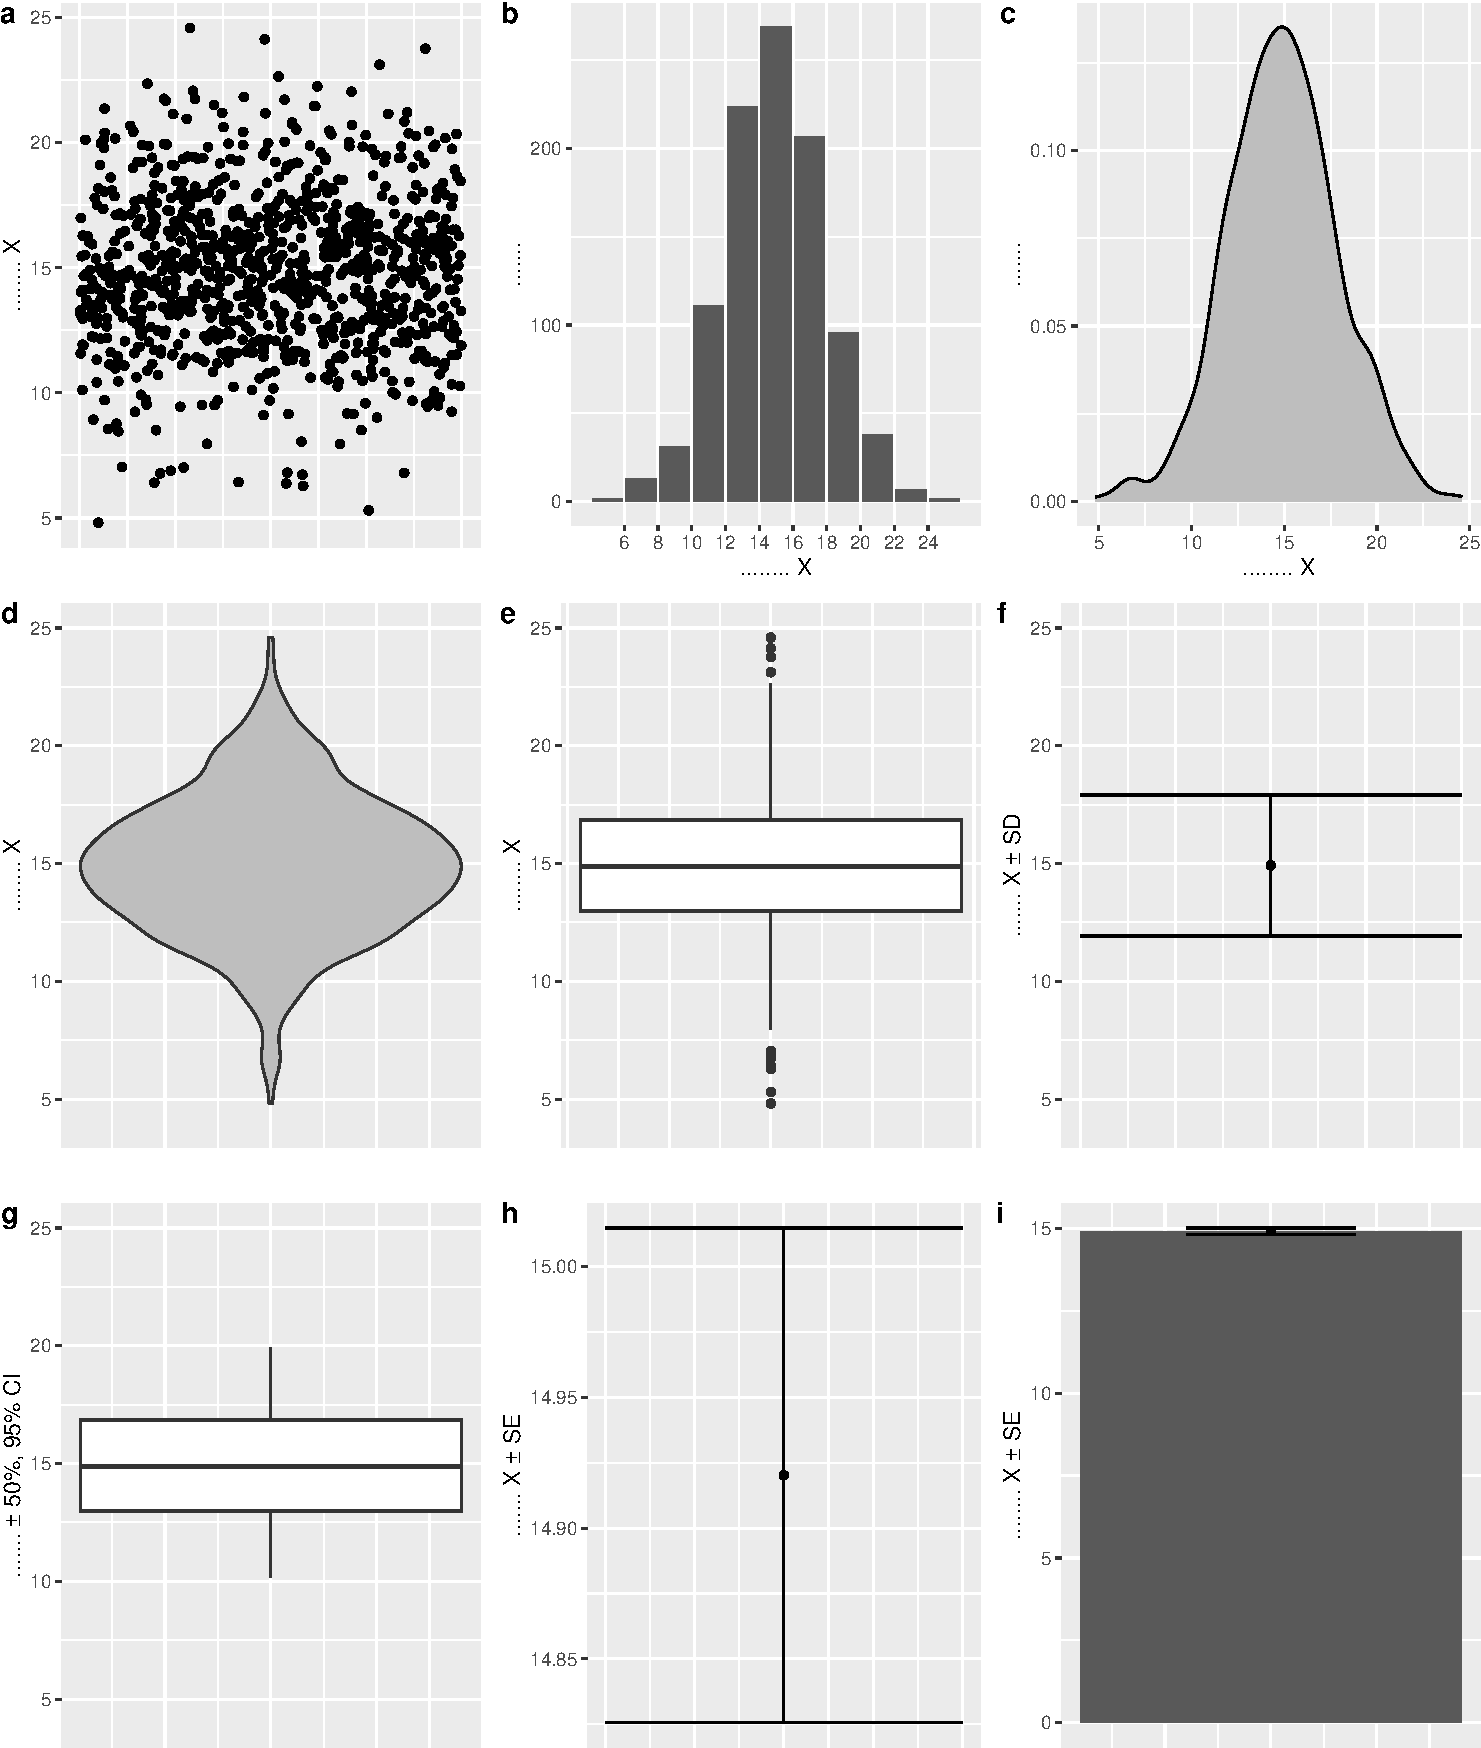
\includegraphics{bookdown-demo_files/figure-latex/fig-3-10-1.pdf}
\caption{\label{fig:fig-3-10}Різноманітні способи зобразити розподіл змінної: \textbf{(a)} хмара точок спостережень - найкращий спосіб зобразити сирі даних, якщо точок відносно небагато; \textbf{(b)} гістограма - колонки відповідають рівномірним діапазонам значень; \textbf{(c)} ядрова оцінка густини розподілу, своєрідна неперевна гістограма, що є кращою альтернативою гістограмі у випадку континуальних змінних; \textbf{(d)} `скрипко-графік' (violin plot) є дзеркальним відображенням ядрової оцінки розподілу; \textbf{(e)} класичний `коробко-графік' (boxplot) де жирна центральна лінія відповідає медіані, межі коробки - міжквартильному розмаху (між 25- та 75-тими перцентилями), межі вусів - розмаху даних без `викидів', а окремі точки - власне викидам (спостереження, що потрапили за межі 1.5 міжквартильного розмаху від 25- чи 75-ого перцентилю); \textbf{(f)} відображення середнього арифметичного і відхилення у формі стандартного відхилення; \textbf{(g)} 2.5-, 25-, 50-, 75-, та 97.5-ті перцентилі, які можуть сприйматися як довірчі інтервали розподілу (але не його середнього); \textbf{(h)} відображення середнього арифметичного і відхилення у формі стандартної помилки - зверніть увагу на шкалу, розмах вусів набагато менший за інші за рахунок значного розміру вибірки; \textbf{(i)} відверто найгірший варіант - `динаміто-графік' (dynamite plot), який малює колонку чогось (на відміну від гістограми, ця колонка рідко має будь-який зміст, наприклад, у вибірці нема значень нижче за 4, але зона від 0 до середнього все одно замальована) із `вусами' стандартної помилки.}
\end{figure}

Зображення розподілу вибірок часто необхідно для порівняння двох (чи більше) вибірок. Наприклад, уявіть вибірки \(A\) і \(B\), які відповідають промірам певного параметру (наприклад, маси тіла) в двох групах (скажімо, субпопуляціях виду). Залежно від того, чому відповідають вуса графіків, висновок із їх візуального зображення відрізнятиметься:

\begin{itemize}
\item
  якщо вуса \textbf{SD} двох вибірок перекриваються між собою, це не може бути достатнім доказом статистичної відмінності між вибірками (необхідні додаткові тести, наприклад, t-тест Ст'юдента або непараметричний аналог);
\item
  якщо вуса \textbf{SE} перекриваються і дві вибірки \emph{мають однакові розміри}, статистичної відмінності між вибірками, скоріш за все, немає; якщо вуса не перекриваються, необхідне додаткове тестування;
\item
  якщо вуса \textbf{95\% CI} перекриваються, необхідне додаткове тестування; якщо ж вони не перекриваються, скоріш за все, існує істотна різниця між вибірками.
\end{itemize}

Загалом, графічне зображення розмаху вибірок викликає чимало плутанини із висновками (\href{https://doi.org/10.1093/jis/3.1.34}{Payton et al.~2003}, \href{https://doi.org/10.1037/1082-989X.10.4.389}{Belia et al.~2005}, \href{https://doi.org/10.1083/jcb.200611141}{Cumming et al.~2007}). Порадою слугуватиме завжди зазначати які саме метрики розмаху зображені й проводити додаткове статистичне тестування гіпотез.

\section{Тестування гіпотез}\label{basic-hypotheses}

\subsection{Статистична гіпотеза}\label{hypothesis}

Статистичне тестування гіпотез має багато спільного із філософією науки. \textbf{Гіпотеза} є припущенням, яке може бути істинним або ні. Будь-яке твердження може бути гіпотезою (наприклад, ``гроза є виявом злості бородатого дядька на небі'' є валідною гіпотезою), однак наукова гіпотеза має бути такою, яку можливо емпірично перевірити (див. \href{https://uk.wikipedia.org/wiki/\%D0\%A1\%D0\%BF\%D1\%80\%D0\%BE\%D1\%81\%D1\%82\%D0\%BE\%D0\%B2\%D1\%83\%D0\%B2\%D0\%B0\%D0\%BD\%D1\%96\%D1\%81\%D1\%82\%D1\%8C}{критерій спростовуваності Поппера}). В процесі наукового пізнання так чи інакше доводиться приймати чи відхиляти гіпотези залежно від наявних даних, однак варто пам'ятати що жодна гіпотеза не є істиною: навіть якщо всі попередні експерименти підтримують робочу гіпотезу, це не означає що наступний експеримент також її підтримає.

Статистичні гіпотези є прикладами гіпотез, особливістю яких є дуже формальний чисельний їх опис. Для кожної статистичної гіпотези має бути можливість записати її у вигляді рівняння, нерівності, чи логіки. Гіпотеза ``гроза є виявом злості бородатого дядька на небі'' не є валідною статистичною гіпотезою, однак її можна переформулювати в ``ймовірність виникнення грози лінійно асоційована із густиною злих бородатих дядьків в об'ємі неба''. Так, методологічно таку гіпотезу все одно перевірити складно, але тепер у неї є математична складова, тож її можливо перевірити.

Статистичні гіпотези зазвичай є доволі простими твердженнями, аби їх можна було перевірити. На практиці, це часто означає пошук балансу між поглибленою трансформацією даних й тестуванням простої гіпотези. Застосовуючи \href{https://uk.wikipedia.org/wiki/\%D0\%91\%D1\%80\%D0\%B8\%D1\%82\%D0\%B2\%D0\%B0_\%D0\%9E\%D0\%BA\%D0\%BA\%D0\%B0\%D0\%BC\%D0\%B0}{принцип Оккама}, якщо декілька статистичних гіпотез відповідають ідентичній науковій гіпотезі і не мають суттєвої різниці між собою, варто обирати найпростішу статистичну гіпотезу. Наприклад, якщо ви намагаєтесь порівняти вибірки мас тіла в двох субпопуляціях виду, \(A\) і \(B\), і припускаєте що між ними є істотна різниця, існує декілька способів сформулювати статистичну гіпотезу: \textbf{(1)} всі значення в \(A\) більші/менші за всі значення в \(B\) (не є хорошою гіпотезою, адже вона занадто консервативна -- спрацює тільки коли дві хмари точок не перетинаються -- і не є занадто простою, адже включає дві статистичні гіпотези \(a_i > b_i \forall a_i, a_b\) та \(a_i < b_i \forall a_i, a_b\)); \textbf{(2)} середнє значення вибірки \(A\) більше/менше за середнє значення \(B\) (менш консервативна, але все ще складна гіпотеза, що включатиме дві простіші гіпотези \(\bar{a} > \bar{b}\) і \(\bar{a} < \bar{b}\)); \textbf{(3)} середнє значення \(A\) не дорівнює середньому значенню \(B\) (включає лише одну елементарну гіпотезу \(\bar{a} \neq \bar{b}\)); \textbf{(4)} різниця між середніми значеннями вибірок не дорівнює нулю (мабуть, є найпростішою гіпотезою, до якої можна звести це питання про маси тіла в субпопуляціях, \((\bar{a} - \bar{b}) \neq 0\)).

\subsection{Нульовий розподіл}\label{nulldistr}

Тестування статистичних гіпотез є доволі цікавим і, певною мірою, контрінтуїтивним процесом. Зазвичай, тести не кажуть ``так, ваша статистична гіпотеза має право на життя'', а виходять із протилежного твердження -- \textbf{нульової гіпотези} (\emph{null hypothesis}), і, відтак, радше кажуть ``не знаю як щодо вашої статистичної гіпотези, але альтернатива їй взагалі не підтверджується наявними даними''. Відтак, для кожної статистичної гіпотези (твердження \(H\)) існує певна нульова гіпотеза, яка намагається пояснити дані із припущення того, що \(H\) не відповідає дійсності (позначимо нульову гіпотезу як \(H_0\)). Як альтернатива нульовій гіпотезі існує \textbf{альтернативна гіпотеза} (\emph{alternative hypothesis}) \(H_A\), яка робить твердження протилежне до \(H_0\) і, відтак, узгоджується із \(H\).

Навіщо це потрібно? Візьмемо до уваги попередній приклад: нашою науковою гіпотезою є те, що особини субпопуляцій А і B відрізняються масою тіла. Для перевірки цієї наукової гіпотези ми формулюємо чітку статистичну гіпотезу \(H: (\bar{a} - \bar{b}) \neq 0\). Як перевірити цю статистичну гіпотезу? Можна, звісно, порахувати середні двох вибірок, і можна гарантувати що їх різниця не дорівнюватиме нулю навіть якщо вони не надто сильно різняться -- отримати вибірки із ідентичними середніми арифметичними дуже малоймовірно. Відтак, ця різниця буде відрізнятись від нуля, і для перевірки статистичної гіпотези необхідно зрозуміти яка різниця між середніми є достатньо великою, аби не вважатись просто статистичним шумом. В цій ситуації у нас є дві взаємозаперечні статистичні гіпотези: нульова \(H_0: (\bar{a} - \bar{b}) = 0\) та альтернативна \(H_A: (\bar{a} - \bar{b}) \neq 0\). Відтак, для відповіді на попереднє питання необхідно знати, який розподіл би мала різниця між середніми \((\bar{a} - \bar{b})\) за умови що \(H_0\) є істинною. Цей розподіл можна назвати нульовим (null distribution), із яким можна порівняти спостережене значення \((\bar{a} - \bar{b})\) і вирішити чи ``так, спостережена різниця набагато більша від випадкового шуму навколо нуля в нульовому розподілі'' (відповідно, відхилити \(H_0\) та прийняти \(H_A\)) або ``ні, спостережена різниця настільки незначна, що її можна було б очікувати навіть якщо насправді різниці нема'' (відхилити \(H_A\) та прийняти \(H_0\)).

За усієї своєї простоти, адекватний статистичний аналіз неможливий без адекватної нульової моделі (\href{https://www.jstor.org/stable/2096971}{Harvey et al.~1983}) -- і ця тема настільки важлива, що їй присвячені цілі книги (\href{https://www.uvm.edu/~ngotelli/nullmodelspage.html}{Gotelli \& Graves 1996})! Готеллі визначає \textbf{нульову модель} як ``\emph{модель, що генерує тренди на підставі рандомізованих екологічних даних чи випадкової вибірки із відомого чи уявного розподілу {[}\ldots{]} створеного для утворення трендів, які можна було би очікувати за відсутності певного механізму {[}в якому ми зацікавлені{]}}''.

Цікавим екологічним прикладом є відомий факт того, що біологічне різноманіття поблизу екватору нашої планети набагато вище порівняно із різноманіттям поблизу полюсів. Існує декілька наукових гіпотез, що пояснюють це спостереження: \textbf{(1)} продуктивність екосистем поблизу екватору вища, відповідно, є більше ресурсів для більшої кількості особин, що означає більше видів (\href{https://doi.org/10.1111/j.1461-0248.2004.00671.x}{Currie et al.~2004}); \textbf{(2)} тропіки є найбільшим біомом, тож є більше площі для підтримки більшої кількості видів (\href{https://doi.org/10.2307/3546528}{Rosenzweig \& Sandlin 1997}); \textbf{(3)} тропіки є старішим біомом, відповідно, було більше часу для видоутворення (\href{https://doi.org/10.1146/annurev-ecolsys-112414-054102}{Fine 2015}); \textbf{(4)} навколо тропіків темпи видоутворення вищі, а вимирання -- нижчі (\href{https://doi.org/10.1111/j.1461-0248.2007.01020.x}{Mittelbach et al.~2007}). Яку нульову модель використати для статистичної перевірки цих гіпотез? Мабуть, рівномірний розподіл різноманіття видів не є найкращою моделлю зважаючи на те, що навколо полюсів менше площі, та й не зрозуміло як врахувати форму планети тощо. Натомість, найпростішою нульовою моделлю варто вважати ефект середнього домену (mid-domain effect): якщо випадкові ареали видів розподілені між полюсами випадково, то суто із геометричних причин більше ареалів перетинатимуться десь між полюсами, й, відповідно, кількість видів буде найбільша посередині, коло екватору (Рис. \ref{fig:fig-3-11}).

\begin{figure}
\centering
\includegraphics{images/mid_domain.png}
\caption{\label{fig:fig-3-11}Ілюстрація ефекту середнього домену для пояснення розподілу біологічного різноманіття на планеті олівцями в коробці: якщо ареали видів випадкових діапазонів широт випадково розподілені між полюсами, то найбільше перетинів видів існуватиме поблизу полюсу. Фіолетові комірки відповідають кількості пересікань із олівцями за горизонталлю.}
\end{figure}

\subsection{Тестування гіпотез}\label{pval}

Суть будь-якого статистичного тесту полягає в оцінці певної статистики тесту (метрики) і оцінці значущості цієї метрики для висновку щодо істинності статистичної гіпотези за певного нульового розподілу. Залежно від парадигми статистичного аналізу, існують різні способи отримати нульовий розподіл. Наприклад, параметричні тести виходять із багатьох припущень і виводять параметричні нульові розподіли. Саме тому настільки важливо дотримуватись припущень тестів (вибірки мають бути нормально розподілені, мати однакові параметри варіації, бути незалежними тощо -- в кожного тесту свій набір припущень).

Результатом статистичного тесту, зазвичай, є оцінка метрики тесту і асоційоване \(p\)-значення -- cвящений грааль і наріжний камінь всякого аналізу, який всі хочуть оцінити але не всі знають що то таке. Мета статистичного тесту -- це оцінити наскільки ймовірно було би отримати певні результати тесту якщо нульова гіпотеза є істинною. Статистичне тестування подібне до судового процесу. Уявіть собі, що підсудного звинувачують у скоєнні злочину (нульова гіпотеза за презумпції невинуватості -- підсудний невинний, альтернативна -- підсудний винний). Перед судом постає відповідальна й непроста задача прийняти рішення щодо винуватості підсудного за наявних даних. Реальність же може відповідати одному з двох варіантів: або підсудний справді вчинив злочин, або ні.

\begin{itemize}
\item
  Якщо підсудний справді не вчиняв злочину (нульова гіпотеза істинна),

  \begin{itemize}
  \item
    рішення суду щодо винуватості підсудного (хибно-позитивний результат) відправить невинну людину за ґрати, або
  \item
    рішення суду щодо невинуватості (дійсно-негативний результат) залишить і підсудного, і суспільство задоволеними,
  \end{itemize}
\item
  якщо ж підсудний насправді вчинив злочин (альтернативна гіпотеза істинна), то

  \begin{itemize}
  \item
    рішення суду щодо винуватості підсудного (дійсно-позитивний результат) виллється у відбування заслуженого покарання, або
  \item
    рішення суду щодо невинуватості (хибно-негативний результат) відправить злочинця на волю, що є небезпечним для суспільства.
  \end{itemize}
\end{itemize}

Відтак, в такому уявному судовому процесі, залежно від реальності, можна припуститись однієї з двох критичних помилок:

\begin{itemize}
\item
  \textbf{помилки першого роду} -- відправити невинну людину за ґрати -- прийняти альтернативну гіпотезу, коли нульова є істинною, або
\item
  \textbf{помилки другого роду} -- відпустити злочинця на волю -- прийняти нульову гіпотезу, коли альтернативна є істинною.
\end{itemize}

Яка із цих помилок є страшнішою, мабуть, є філософським питанням, і кожне суспільство нехай відповідає на нього самостійно. В науці ж помилка першого роду відповідатиме видаванню за істину доказів, які не відповідають дійсності; в той час як помилка другого роду -- ігноруванню фактів. Як на мене, помилка першого роду шкодитиме науковому знанню сильніше.

Якби істина була відома, тоді в кожній парі нульової-альтернативної гіпотез можна було би оцінити дві ймовірності:

\begin{itemize}
\item
  \(\alpha = P(\text{помилка I роду} = P(\text{відхилити } H_0| H_0 \text{ істина})\), яку ще називають \textbf{рівнем значущості} (\emph{significance level}), та
\item
  \(\beta = P(\text{помилка II роду} = P(\text{не відхилити } H_0| H_0 \text{ хибна})\).
\end{itemize}

Два значення \(\alpha\) і \(\beta\) є зворотньо пов'язаними (Рис. \ref{fig:fig-3-12}): збільшення одного значення зменшить інше. Відтак, завдання відповідального статистичного аналізу -- збалансувати \(\alpha\) і \(\beta\), знайти якесь максимальне значення \(\alpha\), яке ми можемо толерувати. На практиці, за таке значення часто приймають \(\alpha = 0.05\) (за незалежного повторення 20 експериментів, ми очікуємо принаймні одного хибно-позитивного результату). Втім, критичне значення \(\alpha\) для будь-якого тесту повинне враховувати баланс між \(\alpha\) і \(\beta\), тим, наскільки небажаними є помилки першого та другого роду. Отже, потрібно завжди пам'ятати що порогове значення \(\alpha = 0.05\) є лише умовністю.

Цікавою метрикою тесту, яку варто побічно згадати, є також \textbf{потужність тесту} (\emph{power}) \((1 - \beta)\). Аналіз потужності (\emph{power analysis}) є поширеним методом знаходження мінімального розміру вибірки для адекватної інтерпретації результатів статистичного тесту. Цей тип аналізу допоможе відповісти на питання ``якщо я хочу провести {[}цей конкретний статистичний тест{]} із рівнем значущості {[}\(\alpha\){]}, то який мінімальний розмір вибірки потрібно було би набрати на стадії збору даних?''.

\begin{figure}
\centering
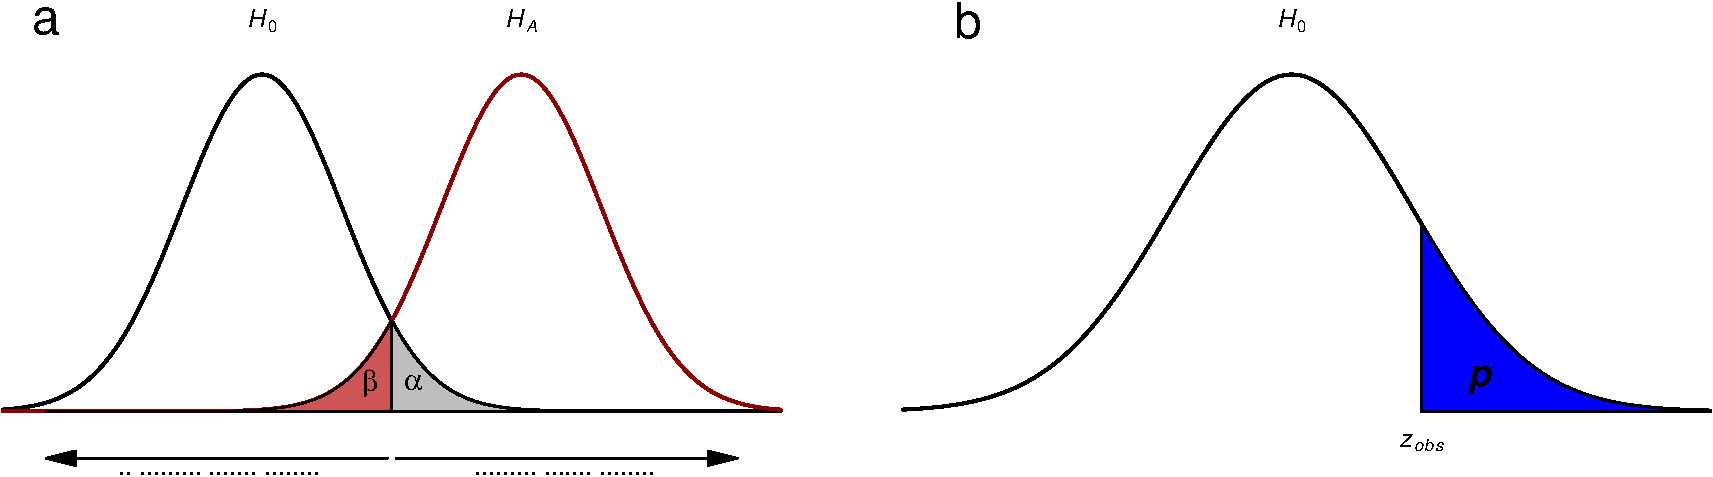
\includegraphics{bookdown-demo_files/figure-latex/fig-3-12-1.pdf}
\caption{\label{fig:fig-3-12}\emph{(a)} Уявімо, що можливо оцінити розподіл статистики тесту \(z\) за нульової (\(H_0\)) та альтернативної (\(H_A\)) гіпотез. Тоді було би можливо оцінити пов'язані ймовірності припуститися помилки першого роду (\(\alpha\), хибно-позитивне рішення) та помилки другого роду (\(\beta\), хибно-негативне рішення) як площі під кривими розподілів статистик. За спостереження статистики тесту \(z_{obs}\), \(p\)-значення відповідає ймовірності спостерігати таке ж або більш екстремальне значення статистику за нульової гіпотези.}
\end{figure}

Підхід \textbf{\(p\)-значення} (p-value) у статистичному тестуванні намагається оцінити ймовірність того, що \emph{значення статистики тесту за істинності нульової гіпотези дорівнюватиме або буде ще більш екстремальним порівняно із спостереженим значенням}. Варто зазначити, що на практиці оперують лише точковим спостереженим значенням статистики тесту (наприклад, різницею середніх значень вибірок \((\bar{a} - \bar{b})\)) та нульовим розподілом (як би були розподілені \((\bar{a} - \bar{b})\) якщо \(H_0: \bar{a} = \bar{b}\)?). Відтак, \(p\)-значення каже наскільки можна очікувати отриманого результату тесту за нульової гіпотези. Якщо ця ймовірність дуже маленька (наприклад, менше за обране порогове значення \(\alpha\)), тоді варто нульову гіпотезу відхилити й існують підстави вважати, що між двома вибірками є істотна різниця. Якщо ж ця ймовірність значна, тоді немає підстав вважати, що отримані результати є чимось більшим аніж статистичним шумом за нульової гіпотези.

Варто звернути увагу на поняття \textbf{\emph{двосторонніх та односторонніх тестів}} (\emph{two-sided}, \emph{upper-tail one-sided}, \emph{lower-tail one-sided}), які відповідають чітко сформульованій альтернативній гіпотезі. Наприклад, якщо ми перевіряємо факт різниці між двома середніми, то альтернативна гіпотеза виглядає як \(H_A: \bar{a} \neq \bar{b} \Leftrightarrow (\bar{a} - \bar{b}) \neq {0}\), отже, зони відхилення нульової гіпотези будуть знаходитись по обидва боки нульового розподілу із ймовірностями \(\alpha/2\). Якщо ж є підстави вважати що одне середнє більше за інше, альтернативна гіпотеза виглядатиме як \(H_A: \bar{a} > \bar{b} \Leftrightarrow (\bar{a} - \bar{b}) > {0}\) або \(H_A: \bar{a} < \bar{b} \Leftrightarrow (\bar{a} - \bar{b}) < {0}\). Відповідно, в такому випадку зона відхилення нульової гіпотези буде знаходитись у верхньому або нижньому хвості нульового розподілу і її ймовірність становитиме \(\alpha\).

Отже, тестування статистичної гіпотези включає наступні кроки:

\begin{itemize}
\item
  формулювання нульової \(H_0\) та альтернативної \(H_A\) гіпотез,
\item
  вибір критичного значення рівня значущості \(\alpha\),
\item
  отримання вибірки достатнього розміру і обчислення статистики обраного тесту \(z\),
\item
  порівняння спостереженої статистики тесту із нульовим розподілом\footnote{нульовий розподіл може бути згенеровано в межах параметричного тесту (наприклад, як t-розподіл в t-тесті Стьюдента) або пермутаційно.}. Є два поширених способи провести цю операцію:

  \begin{itemize}
  \item
    древній метод: поглянути в таблицю критичних значень за певних параметрів нульового розподілу (\(z_{\alpha}\)) і порівняти спостережену статистику із критичною для певного \(\alpha\),
  \item
    адекватніший підхід: обчислити точне значення для параметризованого нульового розподілу та спостереженої статистики тесту,
  \end{itemize}
\item
  зробити висновки щодо відхилення нульової гіпотези.
\end{itemize}

\subsection{Парадигми статистичного аналізу}\label{paradigms}

Різниця між трьома основними парадигмами статистичного аналізу, їх переваги й недоліки, та чим вони відрізняються доволі влучно описано в підручнику Готеллі та Еллісон \href{https://learninglink.oup.com/access/gotelli-a-primer-of-ecological-statistics-2e}{``Початки екологічної статистики''}. В цьому підрозділі я наводжу лише основні ідеї цих парадигм, але варто пам'ятати, що дослідженню кожної з них можна приділити роки життя.

\subsubsection{Частотницька, або фреквентистська парадигма}\label{ux447ux430ux441ux442ux43eux442ux43dux438ux446ux44cux43aux430-ux430ux431ux43e-ux444ux440ux435ux43aux432ux435ux43dux442ux438ux441ux442ux441ux44cux43aux430-ux43fux430ux440ux430ux434ux438ux433ux43cux430}

Найпоширеніший підхід до статистичного аналізу -- частотницький (\emph{frequentist approach}) -- ґрунтується на припущенні, що ймовірність описує ніщо інше, як частоту подій за безкінечного повторення експерименту, й, відповідно, ми можемо спостерігати лише якусь зліченну кількість подій і на їх підставі спробувати оцінити асоційовані ймовірності. Цей підхід часто спрощує спостережувану реальність до ідеальних моделей (які можуть бути дуже складними математично, але все ж простішими за дійсність), які відображені у параметричних моделях -- математичних функціях із відносно незначною кількістю параметрів. Відтак, і тестування гіпотез базується на нульових розподілах із визначеним математичним формулюванням й параметрами (такими розподілами є, наприклад, нормальний, t-розподіл Стьюдента, F-розподіл Фішера тощо).

Параметричні методи завжди мають набір припущень, і перед застосуванням цих методів завжди необхідно перевіряти чи ваші дані відповідають цим припущенням. Більшість параметричних методів матимуть припущення, що \textbf{(1)} всі спостереження в даних зібрані незалежно й випадково, та \textbf{(2)} дані зібрані із генеральних сукупностей із певним визначеним розподілом. Перше припущення не те щоб є специфічним для частотницької парадигми, а є критичним для експериментального дизайну за будь-якого статистичного підходу: вибір залежних між собою спостережень або невипадковий підбір спостережень викликатиме упередження в даних, тож результати всякого статистичного аналізу не будуть адекватними. Друге припущення найчастіше каже, що вибірки в аналізі повинні бути розподілені нормально.

Існують, звісно, і непараметричні методи, однак їх підхід до визначення ймовірності події залишається незмінним. Непараметричні підходи мають послаблені вимоги до розподілу вибірки і є чудовою альтернативою параметричним тестам коли, скажімо, не вдається підтвердити що ваші дані розподілені нормально. Із непараметричними методами завжди варто бути обережними, оскільки навіть якщо вони є надійними (robust) за порушення припущення про розподіл даних, вони є чутливими до всіх інших припущень\footnote{наприклад, для порівняння середніх двох вибірок хорошим вибором статистичного тесту є t-тест Стьюдента. Однак якщо ваші дані не розподілені нормально, вам можуть порадити тест Вілкоксона (Wilcoxon signed-rank test) або тест Манна-Вітні (Mann--Whitney U test). Мало хто знає, втім, що ці тести дуже чутливі до власних припущень: тест Вілкоксона працює лише для незалежних пар залежних (в межах пар) значень, а тест Манна-Вітні передбачає \emph{ідентичні} розподіли між двома групами за нульової гіпотези.}.

\subsubsection{Баєсівська парадигма}\label{ux431ux430ux454ux441ux456ux432ux441ux44cux43aux430-ux43fux430ux440ux430ux434ux438ux433ux43cux430}

Баєсівська парадигма є складнішою для інтуїтивного розуміння і вимагає більшої підготовки. Крім того, я неодноразово чув думку, що Баєсівський метод -- то часто лише модний спосіб тестувати гіпотезу, для якої звичайний параметричний тест дав би таку ж відповідь. Філософія Баєсівського підходу полягає в тому, що часто в розпорядженні існують попередні дані щодо тестованої гіпотези. У частотницькій парадигмі кожен окремий експеримент відбувається ``наосліп'', адже існує припущення, що кожен експеримент отримає якусь репрезентативну вибірку із генеральної сукупності і із його результатів можна судити про тренди в самій генеральній сукупності. Однак, якщо ви проводите експеримент, подібний до якого вже хтось колись проводив, то чи не розсудливіше врахувати ті попередні, \emph{пріорні} дані?

Баєсівський аналіз намагається поглибити наші знання щодо наукової гіпотези із кожним експериментом із врахуванням попередніх даних, що, в цілому, відповідає сучасному науковому підходу: із кожним експериментом ми шліфуємо наявне наукове знання. Скажімо, ми намагаємось оцінити якийсь параметр в генеральній сукупності. Першим кроком у Баєсівському аналізі було би змиритись із думкою про те, що якщо ми намагаємось оцінити цей параметр і його оновлене оцінене значення, скоріш за все, буде відрізнятись від пріорної оцінки, то цей параметр є не фіксованим значенням, а, радше, розподілом значень. Із попередніх експериментів мають бути наявні оцінки розподілу параметру, тож цей розподіл ми назвемо \emph{пріорним}, і тепер нашим завданням є оцінити \emph{постеріорний} розподіл параметру за даних нового експерименту, що можна зробити із застосуванням теореми Баєса:

\[P(\text{гіпотеза}|\text{дані}) = \frac{P(\text{гіпотеза})P(\text{дані}|\text{гіпотеза})}{P(\text{дані})}\]

Отже, якщо частотницькі методи питають \emph{яка ймовірність отримати значення статистики рівне або більш екстремальне за спостережене значення в наявних даних, якщо нульова гіпотеза істинна}, то Баєсівський підхід намагається відповісти \emph{яка ймовірність гіпотези про статистику тесту за наявних даних}. У цій формулі \(P(\text{гіпотеза}|\text{дані})\) називають \textbf{постеріорною ймовірністю}, \(P(\text{гіпотеза})\) -- \textbf{пріорною ймовірністю}, \(P(\text{дані}|\text{гіпотеза})\) -- \textbf{\hyperref[mle]{правдоподібністю}} (що відображає ймовірність спостереження цього конкретного набору даних якщо гіпотеза істинна), в той час як знаменник \(P(\text{дані})\) у Баєсівській теоремі є лише нормалізуючою константою (ймовірність даних за усіх можливих гіпотез), якою можна знехтувати і переписати вираз як

\[P(\text{гіпотеза}|\text{дані}) \propto P(\text{гіпотеза})P(\text{дані}|\text{гіпотеза})\]

Аби ще сильніше ускладнити інтуїтивне розуміння цієї парадигми, кожну із ймовірностей у цій формулі варто уявляти не як точкове значення ймовірності, а як \hyperref[pdfs]{розподіли густини ймовірності}. Вибір \emph{пріорного розподілу} залежить від попередньо існуючих даних: навіть із описових даних можна спробувати визначити певний виправданий розподіл. Якщо ж цього не вдається зробити, альтернативою (яку дуже часто використовують) є визначення \emph{неінформативного розподілу} (uninformative prior), наприклад, нормального розподілу із настільки високим параметром \(\sigma^2\), що на локальних діапазонах він апроксимує до плаского рівномірного розподілу. У виборі неінформативного пріорного розподілу й криється критика повсюдного застосування Баєсівської парадигми: якщо в моделі відсутнє адекватно визначене пріорне знання, то Баєсівський аналіз не має жодних переваг над частотнитцькими методами (\href{https://doi.org/10.1111/oik.05985}{Lemoine 2019}). Відтак, вибір пріорного розподілу повинен бути обґрунтованим.

Подальші кроки вимагають оцінки функції правдоподібності даних за істинності гіпотези (\(P(\text{дані}|\text{гіпотеза}\)) та нормалізуючої константи інтегрованої правдоподібності (\emph{marginal likelihood}), що іноді можна зробити аналітично, але, зазвичай, розв'язується за допомогою алгоритмів ітеративно. На виході Баєсівський підхід повертає розподіл постеріорної ймовірності. Як із розподілу зробити висновок? Поширеним інструментом є оцінка \textbf{імовірного інтервалу} (\emph{credibility interval}, не плутати із довірчим інтервалом, \emph{confidence interval}), наприклад, 95\% імовірного інтервалу як 2.5\%- і 97.5\%-ті перцентилі постеріорного розподілу. Розташування спостереженої статистики тесту відносно 95\% імовірного інтервалу постеріорного розподілу (в межах або за межами), відтак, дає підставу зробити висновок щодо статистичної гіпотези.

В контексті Баєсівської парадигми варто згадати методи Монте-Карло ланцюгів Маркова (\emph{Markov chain Monte Carlo}, MCMC). \textbf{Процес Маркова}, або \textbf{ланцюг Маркова} -- це такий процес, в якому об'єкт в момент часу має певне значення, і переходить в інший стан в наступний момент часу. Такі стани можуть бути як неперервною змінною, так і дискретною; найпростіше для розуміння уявляти скінченний, бажано невеликий, набір дискретних станів. Популярним прикладом є погодні умови в певний день. Скажімо, набір можливих станів в цій системі є \(\{\text{сонячно}, \text{хмарно}, \text{дощ}\}\), і кожен день приймає один із цих станів. Якби такий процес був Марковським, то в кожен окремий день ймовірність стану залежить тільки від стану в попередній день; \emph{випадковий процес, в якому ймовірність стану в момент часу за відомої послідовності станів в усі попередні кроки залежить тільки від стану протягом останнього попереднього кроку} називають таким, що має властивість Маркова. Ланцюг Маркова описується набором ймовірностей переходу від станів. Ланцюги Маркова часто зображають у вигляді графічних ланцюгів (Рис. \ref{fig:fig-3-13}), в той час як їх математична репрезентація виглядає як \hyperref[matrices]{матриця} ймовірностей переходів -- \textbf{матриця переходів} \(\mathbf{T}\) (\emph{transition matrix}). В таких матрицях рядки відповідають попереднім станам, а колонки -- наступним. Сума ймовірностей переходів із певного стану (сума рядків) повинна дорівнювати одиниці.

\begin{figure}
\centering
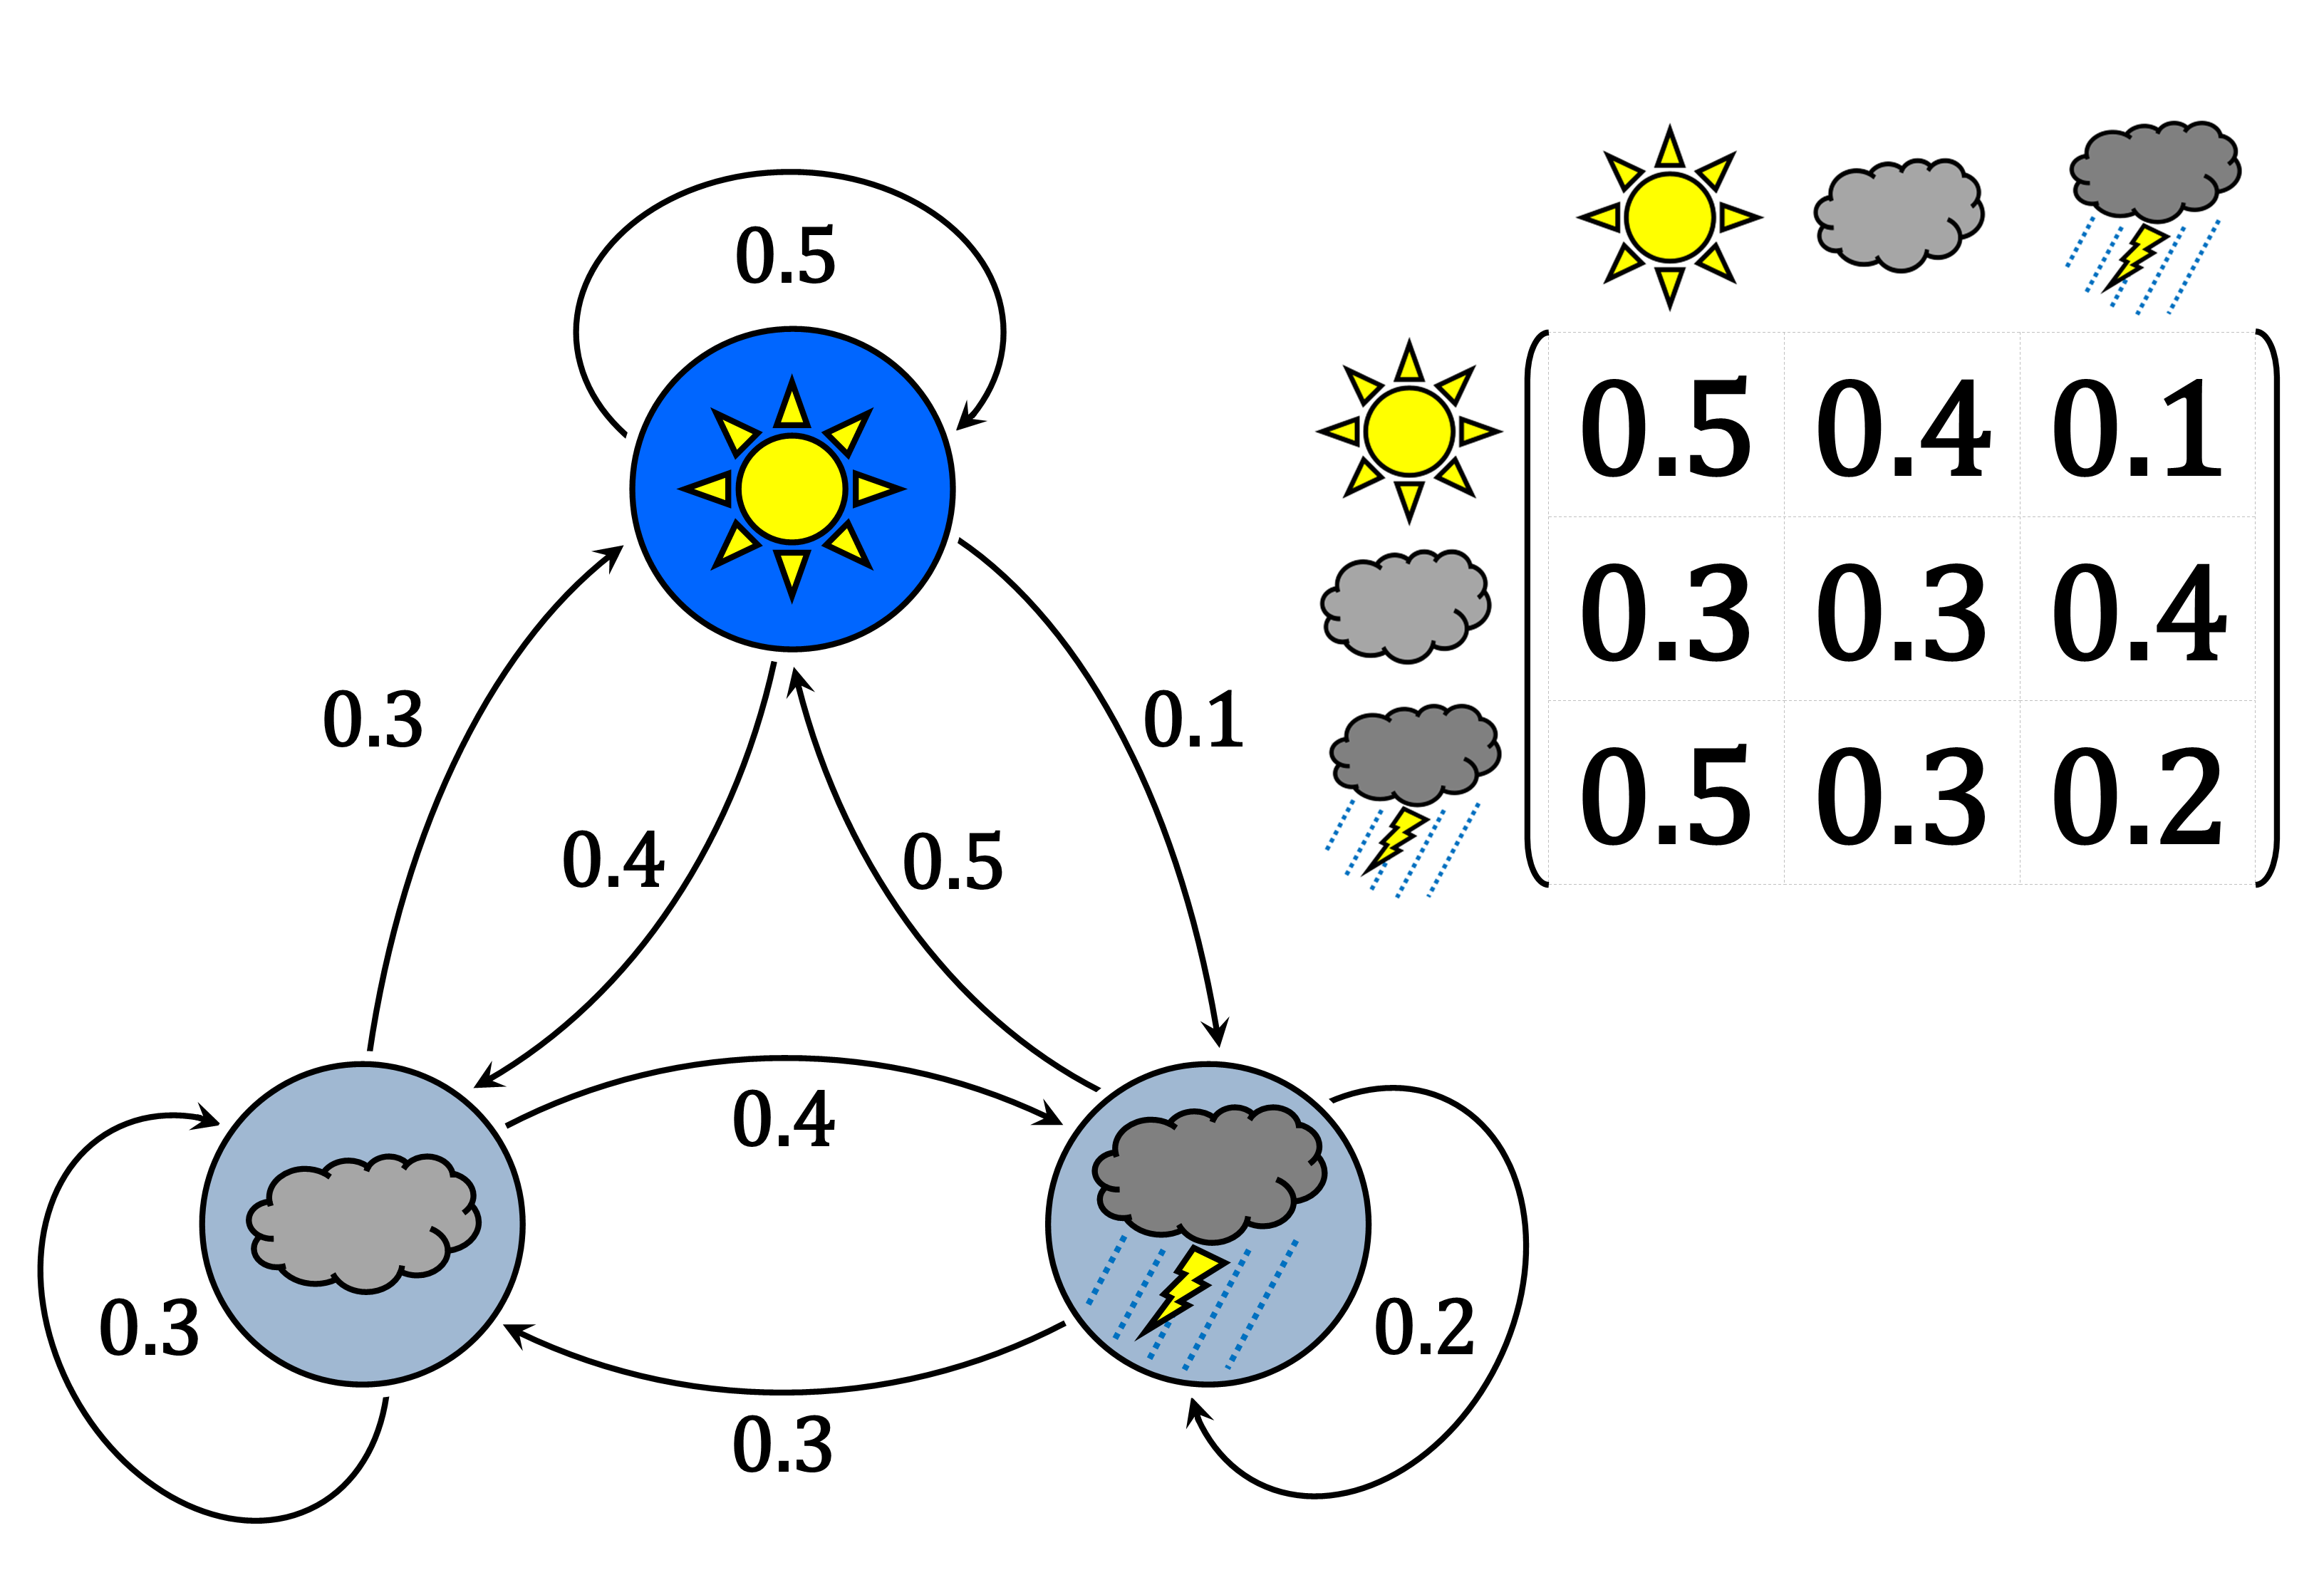
\includegraphics{images/mc.png}
\caption{\label{fig:fig-3-13}Гіпотетичний ланцюг Маркова у графічному вигляді та у вигляді матриці ймовірностей переходів, що описує погоду протягом дня як один із трьох можливих станів. Після сонячного дня варто очікувати сонячний день, після хмарного -- дощів, після дощового -- сонячного тощо.}
\end{figure}

Звісно, розвиток подій в ланцюзі Маркова може залежати від розподілу станів на стадії його ініціалізації -- а отже, і на кожному кроці частоту станів можна описати як функцію розподілу ймовірності. Певні ланцюги Маркова можуть досягнути рівноважного стану, коли розподіли ймовірності перестають змінюватись із наступним кроком. Відповідно, \emph{стаціонарним} (\emph{stationary}) розподілом називають такий розподіл \(\vec{\pi}\), для якого справджується умова, що \(\vec{\pi} \mathbf{T} = \vec{\pi}\). Пермутації Монте-Карло ланцюгів Маркова відповідають алгоритмам, які ітерують велику кількість кроків крізь такий Марковський процес, стаціонарний розподіл якого відповідає шуканому розподілу. Найвідомішим є \textbf{алгоритм Метрополіса-Хастінгса} (\emph{Metropolis-Hastings algorithm}) для отримання випадкової вибірки \(X\) із певного складного розподілу або просто функції \(f(x)\), із якої непросто отримати випадкову змінну аналітичним шляхом. В цьому алгоритмі нарощується ланцюг випадкових значень, що на початку алгоритму обирається із заданого пріорного розподілу. На кожному кроці \((i)\) алгоритм бере до уваги значення \(x_{i-1}\) із розподілу попереднього кроку, і будує навколо \(x_{i-1}\) якийсь визначений розподіл \(g(x_{i-1})\) (наприклад, нормальний із фіксованою між кроками варіацією \(\mathcal{N}(\mu = x, \sigma^2)\)). Із цього розподілу обираєтся випадкове значення-кандидат \(x'\) таке що \(x` \sim g(x_{i-1})\) (якщо було обрано нормальний розподіл, то\(x' \sim \mathcal{N}(\mu = x_{i-1}, \sigma^2)\)). Після цього алгоритм обирає, чи взяти до уваги \(x'\), при чому ймовірність вибору значення-кандидата \(x'\) визначається відношенням \(g(x')/g(x_{i-1})\). Якщо обрано \(x'\), то нове значення в розподілі нарощене протягом цього кроку становитиме \(x_i = x'\), якщо ж ні, то \(x_i = x_{i-1}\). Процедура повторюється багаторазово (розряду тисяч разів), і в результаті видає ланцюг \(\{x_1, x_2, x_3, \cdots, x_n\}\). Із цього ланцюга викидається певна кількість перших \(m\) ланок, оскільки в них алгоритм іноді видає невдалі значення -- цей період називають розігрівом (\emph{burn-in}). Залишок ланцюга \(\{x_{m+1}, x_{m+2}, \cdots, x_n\}\) ж утворює вибірку, розподіл якої апроксимує до шуканого. Якщо шуканий розподіл відповідає постеріорному розподілу в Баєсівській парадигмі, а функція \(g(x)\) пропорційна до функції правдоподібності даних за тестованої гіпотези, то цей алгоритм є вдалим вибором для Баєсівського аналізу. В мережі нескладно знайти \href{https://blog.djnavarro.net/posts/2023-04-12_metropolis-hastings/}{приклади} простих алгоритмів МСМС на R.

\subsubsection{Пермутаційний аналіз}\label{ux43fux435ux440ux43cux443ux442ux430ux446ux456ux439ux43dux438ux439-ux430ux43dux430ux43bux456ux437}

Принцип роботи МСМС навіює певний настрій ітеративного стилю статистичного аналізу: якщо не вдається вирішити проблему аналітично, просто напишіть алгоритм, який оцінить оптимальне рішення! Ба більше, як вже було згадано вище, параметричні та непараметричні тести працюють лише коли дані відповідають всім припущенням цих тестів. Якщо це не відповідає дійсності, то ітеративні обчислення також можуть стати в нагоді, варто лише пам'ятати процедури тестування гіпотез.

Уявіть два угруповання, \(A\) і \(B\). Кожне угруповання описується як кількість особин певного виду (обмежимо \(\gamma\)-різноманіття, тобто сумарне різноманіття між угрупованнями, до десяти видів), що для цієї ілюстрації ми згенеруємо випадково із розподілу Пуасона.

\begin{Shaded}
\begin{Highlighting}[]
\NormalTok{comA }\OtherTok{\textless{}{-}} \FunctionTok{rpois}\NormalTok{(}\DecValTok{10}\NormalTok{, }\DecValTok{5}\NormalTok{)}
\NormalTok{comB }\OtherTok{\textless{}{-}} \FunctionTok{rpois}\NormalTok{(}\DecValTok{10}\NormalTok{, }\DecValTok{5}\NormalTok{)}
\end{Highlighting}
\end{Shaded}

Якщо позначити кожен вид, то ми можемо поглянути на ці два угрупованні як на таблицю:

\begin{Shaded}
\begin{Highlighting}[]
\NormalTok{coms }\OtherTok{\textless{}{-}} \FunctionTok{data.frame}\NormalTok{(}\AttributeTok{A =}\NormalTok{ comA, }\AttributeTok{B =}\NormalTok{ comB, }\AttributeTok{row.names =}\NormalTok{ letters[}\DecValTok{1}\SpecialCharTok{:}\DecValTok{10}\NormalTok{])}
\NormalTok{coms}
\end{Highlighting}
\end{Shaded}

\begin{verbatim}
##    A B
## a  5 4
## b 10 4
## c  6 4
## d  7 3
## e  5 7
## f  3 3
## g  7 4
## h  9 2
## i  4 4
## j  3 3
\end{verbatim}

І от питання: наскільки ці угруповання подібні між собою? Для відповіді є цілий набір різноманітних \hyperref[similarity]{індексів подібності}, однак в цьому прикладі можемо обмежитись доволі стародавньою метрикою -- Евклідовою відстанню. Зі школи можна пригадати, що квадрат гіпотенузи дорівнює сумі квадратів катетів. Якщо задуматись, то довжина гіпотенузи є дистанцією між двома кутами прямокутного трикутника, координати яких становлять \((x = \text{довжина катету 2}, y = 0)\) та \((x = 0, y = \text{довжина катету 1})\). Відповідно, цю теорему Піфагора можна використати для розрахунку дистанції між двома точками \(p\) і \(q\) в двовимірному просторі із координатами \((p_1, p_2)\) та \((q_1, q_2)\): \(d_{p, q}= \sqrt{(p_1 - q_1)^2 + (p_2 - q_2)^2}\). Краса Евклідової дистанції в тому, що її формулу можна екстраполювати на будь-яку кількість вимірів (позначимо вимірність як \(n: i = 1, 2, 3, \cdots, n\)): \(d(p, q) = \sqrt{\sum_{i=1}^n (p_i - q_i)^2}\). Евклідова дистанція вказує на те, наскільки два об'єкти близькі один до одного в просторі, і якщо уявити угруповання такими об'єктами, то Евклідову дистанцію можна спробувати використати для оцінки того, наскільки два угруповання подібні один до одного\footnote{Евклідова дистанція не є найбільш поширеним показником подібності угруповань, але в цьому контексті є зручною для прикладу.}.

\begin{Shaded}
\begin{Highlighting}[]
\NormalTok{eucl\_dist }\OtherTok{\textless{}{-}} \ControlFlowTok{function}\NormalTok{(x, y)\{}
  \FunctionTok{sqrt}\NormalTok{(}\FunctionTok{sum}\NormalTok{((x }\SpecialCharTok{{-}}\NormalTok{ y)}\SpecialCharTok{\^{}}\DecValTok{2}\NormalTok{))}
\NormalTok{\}}
\NormalTok{d\_obs }\OtherTok{\textless{}{-}} \FunctionTok{eucl\_dist}\NormalTok{(coms}\SpecialCharTok{$}\NormalTok{A, coms}\SpecialCharTok{$}\NormalTok{B)}
\NormalTok{d\_obs}
\end{Highlighting}
\end{Shaded}

\begin{verbatim}
## [1] 10.90871
\end{verbatim}

І отже ми отримуємо якесь значення дистанції -- нашу статистику. Тепер постає інше питання, що це значення значить? Чи наші угруповання подібні між собою, чи ні? Це є гарним питанням для застосування статистичного тестування, в якому \emph{нульовою гіпотезою} є те, що два угруповання походять із однієї генеральної сукупності (метаугруповання -- множини угруповань), а \emph{альтернативна гіпотеза} -- що два угруповання походять із різних метаугруповань. Для тестування нульової гіпотези не залишається нічого, окрім як отримати нульовий розподіл для наших даних.

Можливо, існує спосіб аналітично знайти розподіл очікуваних Евклідових дистанцій для вибірок із однієї генеральної сукупності, однак вирішення такої задачі вимагатиме чимало часу і ми не знаємо чи це взагалі можливо. Тут у нагоді стає метод \textbf{бутстреп} (\emph{bootstrap}), який дозволяє оцінити нульовий розподіл на підставі наявних даних. Симулювати нульову гіпотезу нескладно: для цього лише необхідно перемішати чисельності видів в спостережених угрупованнях. В цій конкретній ситуації, втім, постає питання адекватних нульових розподілів, адже за нульової гіпотези чисельності видів можуть бути маніпульовані тільки для кожного виду окремо (тобто не буде коректним замінити чисельність виду a в угруповання А чисельністю виду j із угруповання В, адже чисельності видів не є незалежними; втім, це не було би проблемою для незалежних змінних на кшталт результатів морфологічних промірів випадкових особин). Відтак, визначмо функцію, яка перемішуватиме чисельності видів таким чином, що симульована чисельність виду в угрупованні може рівноймовірно походити з угруповання А чи В. Варто зазначити, що для бутстрепу необхідно використовувати процедуру відбору із заміщенням (\emph{sampling with replacement})\footnote{Якщо із вибірки обрати певний елемент, після чого цей елемент не можна обрати ще раз, такий відбір називається відбором без заміщення (\emph{sampling without replacement}). Наприклад, ви намагаєтесь оцінити розподіл кольорів в кошику із кольоровими кульками: у відборі без заміщення кожну кульку дістати можна тільки раз. На противагу, якщо ви дістаєте одну кульку, записуєте її колір, і кладете назад у кошик, це є прикладом відбору із заміщенням. Очевидно, розмір вибірки не може бути більшим за розмір вихідної вибірки за відбору без заміщення, однак може бути більшим за відбору із заміщенням.}.

\begin{Shaded}
\begin{Highlighting}[]
\CommentTok{\# для всяких пермутацій необхідно повернути випадкове зерно до замовчування}
\FunctionTok{rm}\NormalTok{(.Random.seed, }\AttributeTok{envir=}\FunctionTok{globalenv}\NormalTok{())}

\NormalTok{mix\_coms }\OtherTok{\textless{}{-}} \ControlFlowTok{function}\NormalTok{(com)\{}
\NormalTok{  out }\OtherTok{\textless{}{-}} \FunctionTok{apply}\NormalTok{(com, }\DecValTok{1}\NormalTok{, }\ControlFlowTok{function}\NormalTok{(x) }\FunctionTok{sample}\NormalTok{(}\AttributeTok{x =}\NormalTok{ x, }\AttributeTok{size =} \DecValTok{2}\NormalTok{, }\AttributeTok{replace =}\NormalTok{ T)) }\SpecialCharTok{\%\textgreater{}\%} \FunctionTok{t}\NormalTok{() }\SpecialCharTok{\%\textgreater{}\%} \FunctionTok{as.data.frame}\NormalTok{()}
  \FunctionTok{colnames}\NormalTok{(out) }\OtherTok{\textless{}{-}} \FunctionTok{colnames}\NormalTok{(com)}
  \FunctionTok{return}\NormalTok{(out)}
\NormalTok{\}}
\NormalTok{new\_coms }\OtherTok{\textless{}{-}} \FunctionTok{mix\_coms}\NormalTok{(coms)}
\NormalTok{new\_coms}
\end{Highlighting}
\end{Shaded}

\begin{verbatim}
##    A  B
## a  4  4
## b 10 10
## c  6  4
## d  3  3
## e  5  7
## f  3  3
## g  7  7
## h  2  2
## i  4  4
## j  3  3
\end{verbatim}

\begin{Shaded}
\begin{Highlighting}[]
\FunctionTok{eucl\_dist}\NormalTok{(new\_coms}\SpecialCharTok{$}\NormalTok{A, new\_coms}\SpecialCharTok{$}\NormalTok{B)}
\end{Highlighting}
\end{Shaded}

\begin{verbatim}
## [1] 2.828427
\end{verbatim}

Тепер цю операцію можна повторити багато разів, скажімо, десять тисяч разів, аби згенерувати розподіл статистики.

\begin{Shaded}
\begin{Highlighting}[]
\NormalTok{d\_null }\OtherTok{\textless{}{-}} \FunctionTok{numeric}\NormalTok{(}\DecValTok{10000}\NormalTok{)}
\ControlFlowTok{for}\NormalTok{ (i }\ControlFlowTok{in} \DecValTok{1}\SpecialCharTok{:}\DecValTok{10000}\NormalTok{)\{}
\NormalTok{  new\_coms }\OtherTok{\textless{}{-}} \FunctionTok{mix\_coms}\NormalTok{(coms)}
\NormalTok{  d\_null[i] }\OtherTok{\textless{}{-}} \FunctionTok{eucl\_dist}\NormalTok{(new\_coms}\SpecialCharTok{$}\NormalTok{A, new\_coms}\SpecialCharTok{$}\NormalTok{B)}
\NormalTok{\}}
\end{Highlighting}
\end{Shaded}

Погляньмо на розподіл цієї статистики (чорна лінія відповідає ядерній оцінці густини розподілу) і порівняймо його із спостереженим значенням (червона лінія).

\begin{Shaded}
\begin{Highlighting}[]
\FunctionTok{density}\NormalTok{(d\_null) }\SpecialCharTok{\%\textgreater{}\%} \FunctionTok{plot}\NormalTok{(}\AttributeTok{xlab =} \StringTok{"Евклідова відстань"}\NormalTok{, }\AttributeTok{ylab =} \StringTok{"KDE"}\NormalTok{, }\AttributeTok{main =} \StringTok{""}\NormalTok{)}
\FunctionTok{abline}\NormalTok{(}\AttributeTok{v =}\NormalTok{ d\_obs, }\AttributeTok{lwd =} \DecValTok{2}\NormalTok{, }\AttributeTok{col =} \StringTok{"red"}\NormalTok{)}
\end{Highlighting}
\end{Shaded}

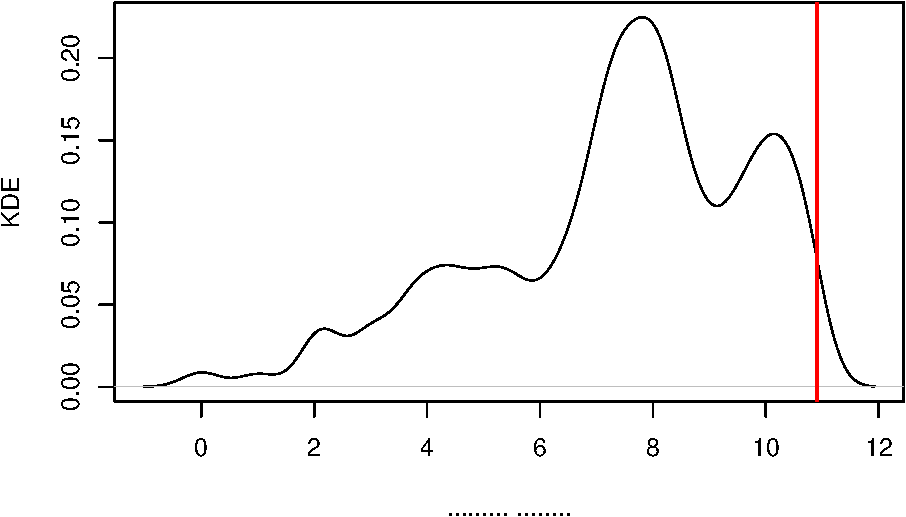
\includegraphics{bookdown-demo_files/figure-latex/unnamed-chunk-15-1.pdf}

Оскільки за нульової гіпотези можна очікувати, що значення відстані наближатиметься до нуля (до того ж, дистанція не може бути негативною), екстремальні значення нульового розподілу відповідатимуть значним позитивним значенням. Ця логіка дозволяє оцінити псевдо-\(p\)-значення як для одностороннього тесту:

\begin{Shaded}
\begin{Highlighting}[]
\FunctionTok{length}\NormalTok{(d\_null[d\_null }\SpecialCharTok{\textgreater{}=}\NormalTok{ d\_obs])}\SpecialCharTok{/}\FunctionTok{length}\NormalTok{(d\_null)}
\end{Highlighting}
\end{Shaded}

\begin{verbatim}
## [1] 0.0084
\end{verbatim}

Отже, в генерованому розподілі нульової вибірки, ймовірність отримати спостережене або більше за спостережене значення статистики \(p \approx 0.01\) (оскільки процес стохастичний, оцінка відрізнятиметься за кожного компілювання), що дозволяє відхилити нульову гіпотезу і стверджувати що два угруповання відрізняються між собою.

Пермутаційні методи є доволі пластичними, адже їх можна застосовувати для будь-яких статистик і будь-яких розподілів вихідних даних. Великим недоліком, втім, є те, що цей метод є комп'ютер-інтенсивним, і для великих наборів даних обчислення вимагатимуть чимало комп'ютерного часу (секунди, хвилини, іноді дні).

\section{Експеримент і модель}\label{stat-models}

За визначенням, модель є спрощеним, узагальненим, концептуальним уявленням про явище реального світу. Моделі ніколи не відображають реальність всеохоплююче, адже природні процеси часто є занадто складними системами аби їх вичерпно описати. Моделі часто також мають певні межі, поза якими адекватне узагальнення не є адекватним. Втім, так чи інакше, моделювання є доволі потужним інструментом тестування гіпотез, без якого екологія не може існувати. Навіть якщо на систему впливають сотні різних чинників, комбінований вплив яких є дуже складним і неочікуваним, моделі із лише декількома змінними часто є достатніми для бодай якого та й висновку.

Для побудування моделі необхідні вхідні емпіричні дані, які в ідеальних умовах мають походити із експерименту -- контрольоване маніпулювання окремого чинника із супутнім спостереженням за поведінкою системи. В екології угруповань та екосистем проведення контрольованого експерименту не завжди є можливими, адже досліджувані системи є дуже великими, однак це не означає що неможливо зібрати дані. Спостереження також може генерувати корисні дані для моделювання. Процедуру збору даних для побудування моделі називають експериментальним дизайном. Адекватний статистичний аналіз неможливий без адекватного експериментального дизайну, якими би потужними чи модними не були статистичні методи.

Уявіть гіпотезу, що частота співання серед самців зяблика залежить від інтенсивності освітлення навколишнього середовища. Для перевірки цієї гіпотези можна розробити дизайн експерименту. Наприклад, в декількох точках розвісити автоматичні звукові рекордери і датчики освітлення. Яких помилок можна припуститись в цьому дизайні? Можна розвісити датчики настільки близько один до одного, що декілька датчиків будуть одночасно записувати одних і тих же особин: в такому випадку спостереження не будуть незалежними, що суперечитиме припущенням більшості статистичних тестів. Можна розвісити датчики освітлення занадто далеко від рекордерів: тоді спостереження не будуть між собою пов'язані, і всякі результати не матимуть жодного сенсу. Можна повісити датчики в екотопі чи континенті, де зяблики не трапляються\ldots{} Гаразд, скажімо, експериментальний дизайн адекватний, дані зібрано, і знайдено взаємозв'язок між інтенсивністю освітлення й частотою співання. Знайдений зв'язок являє собою модель. Які її межі? Наприклад, така модель може передбачити, що в умовах нульового освітлення (в печері) варто очікувати негативної частоти співання, а за дуже інтенсивного освітлення, як-то прямо під прожектором, самець буде співати і не затикатись. Обидва передбаченнями є неадекватними. Крім того, чи експеримент врахував всі можливі фактори? Адже поведінка птахів може бути пов'язаною не тільки із освітленням, а й з температурою, наявністю корму, гніздових територій, інших самців, самок тощо, і навіть коли всі ці фактори враховано, то у одного конкретного зяблика може просто не бути настрою співати. Відтак, наша модель не є вичерпною, і питання лише в тому, чи є статистично значуща роль \emph{тільки} інтенсивності освітлення -- а багатьма іншими факторами іноді варто просто знехтувати.

\subsection{Експериментальний дизайн та псевдореплікація}\label{pseudoreplication}

Уявіть, що ви намагаєтесь дослідити вплив якоїсь хімічної сполуки в ґрунті на процеси росту рослин. Ви відбираєте сотню особин рослин однакового віку та фізіологічного стану із однієї генетичної лінії, висаджуєте кожну рослину в окремий вазон, і виставляєте їх в дві теплиці по п'ятдесят вазонів на теплицю. В одній теплиці ви додаєте однакову кількість хімічної сполуки до кожного вазону, в іншому -- ні. За декілька тижнів настає час зібрати результати, і ви обережно вимірюєте морфологічні параметри кожної рослини: ріст, кількість листків, сумарну площу листків, концентрацію хлорофілу, суху біомасу. Прийшов час проводити статистичну обробку даних, ви дбайливо перевірили розподіли кожної змінної, і еврика! Тест Стьюдента показує значущу відмінність між двома групами за всіма параметрами. Виявляється, додавання цієї хімічної сполуки пов'язане із активнішим ростом рослин. Час подавати заявку на патент?

Не так швидко. Який був розмір вашої вибірки? Сотня особин, тож \(n = 100\)? Чи, оскільки і кожній групі було по п'ятдесят особин, то \(n = 50\)? Насправді, \(n = 2\). Можливо, теплиця із кращим ростом рослин стояла в місці із кращою експозицією до сонячних променів, або під нею зарита труба із теплою водою, або її нещодавно відремонтували і там краща термоізоляція, або вона ближче до виходу й аспіранти постійно ходили в неї на перекур. Можливостей є настільки безліч, що всі їх контролювати із таким експериментальним дизайном неможливо. Жахіття \textbf{змішувальних змінних} (\emph{confounding variable}, таких змінних що впливають і на незалежну, і на залежну змінну, й відтак спричиняють коваріацію між ними без жодного причинно-наслідкового зв'язку) й помилок експериментального дизайну треба завжди мати на увазі. Цей же експеримент став жертвою невдалого дизайну із псевдореплікацією і лише довів ефект теплиці на ріст рослин.

Поняття \textbf{псевдореплікації} (\emph{pseudoreplication}) ввів \href{https://doi.org/10.2307/1942661}{Харлберт 1984 року} і визначив його як ``використання статистичного умовиводу для тестування експериментального ефекту на даних із експериментів де ефект не є реплікованим (хоча вибірки можуть бути реплікованими) або репліканти не є статистично незалежними''. В цьому формулюванні, під ``експериментальним ефектом'' (\emph{treatment}) мається на увазі будь-яке спеціальне відношення до зразків, яке є під питанням в експерименті (наприклад, додавання хімікатів), і яке розділяє вибірку на ``експеримент'' і ``контроль''. Вибірки в експериментальній чи/та контрольній групах можуть бути реплікованими (тобто мати більше за один зразок), але репліканти -- підмножини вибірки, в яких всі елементи отримують однаковий експериментальний ефект -- не обов'язково відповідають цим групам. У прикладі вище реплікантами є не окремі зразки в експериментальній/контрольній групах, а теплиці, адже в межах теплиці експериментальний ефект однаковий. На противагу, якби всі зразки були в одній теплиці, тоді ефект теплиці можна було б елімінувати і кожен окремий вазон майже можна було б вважати реплікантом (майже, адже зразки з однієї теплиці все ще не є статистично незалежними). Ще краще, якщо цього дозволяють ресурси, було б мати множину теплиць в яких випадковим чином розподілені зразки із експериментальної та контрольної груп. В такому випадку ефект теплиць можна було б врахувати в статистичному аналізі, наприклад, за рахунок \textbf{змішаних моделей} (\emph{mixed-effect model}) із рандомним ефектом теплиці.

Визначення Харлберта робить акцент на статистичній незалежності, якої часто дуже складно досягнути. В ідеальному випадку псевдореплікації можна уникнути коли нема підстав вважати, що одні й ті ж чинники впливають на різні зразки. В екології особливу увагу варто приділяти просторовій та часовій незалежності. Якщо дані зібрані із різних просторових точок, можна виправдано очікувати що близькі між собою точки будуть менш незалежними одна від одної порівняно із далекими точками (наприклад, вимірювання вмісту газів в межах міста не будуть незалежними, бо всі зразки є під впливом одного мікроклімату). В таких випадках варто зважати на \textbf{просторову автокореляцію} (\emph{spatial autocorrelation}) -- залежність точок даних від їх взаємного розміщення в просторі -- і використовувати специфічні методи аналізу що враховують цю автокореляцію\footnote{\textbf{автокореляція} -- це кореляція змінної із самою собою, тобто залежність значень у вибірці від інших значень в цій вибірці}. Подібно, вимірювання змінних в часі також не є незалежними, адже значення змінної в момент часу залежить від значень цієї змінної в інші моменти часу (наприклад, середня добова температура сьогодні залежить від температури вчора -- набагато ймовірніше що між цими значеннями незначна різниця, адже різкі перепади температури є відносно рідкісним явищем). Будь-які змінні в часі варто аналізувати за допомогою методів \textbf{часових серій} (\emph{time series}). Варто зважати, що будь-який натяк на відсутність статистичної незалежності у вибірці зводить нанівець використання більшості класичних статистичних тестів, а відтак їх результати не є достовірними.

\subsection{Дані та проблема моделювання}\label{regression}

У житті кожного польовика наступає такий момент, коли стадія планування дослідження (= розробки експериментального дизайну) із усіма врахованими застереженнями щодо псевдореплікації та незалежності спостережень давно позаду, труднощі польових досліджень подолані, все, що могло піти не так, пішло не так і ці помилки виправлені, і можна гордо сказати що збір даних закінчено. В цей момент ейфорія доконаності перспективи прокидатись о 5 ранку і лізти в, як воно завжди буває, найнеочікуваніші місця по об'єкт досліджень швидко заміщується жахом від усвідомлення того, що тепер всі зібрані дані пора би аналізувати. Статистичних тестів існує безліч, і до одного набору даних можна застосувати багато різних методів, більшість із яких видадуть якийсь результат. Тож який підхід обрати? Цей підрозділ не дасть відповіді на це питання, однак може підштовхнути до перших кроків.

Однією ремаркою буде \textbf{формат даних}. Часто на момент оцифровування польових нотаток з'являється спокуса зробити нудну таблицю більш візуально привабливою (наприклад, додати заголовок, виділити клітинки обабіч для нотаток, додати відсотки чи одиниці вимірювання коло значень, вписати декілька значень в одну клітинку тощо). Такий підхід, звісно, дещо спрощує і без того нудний процес оцифровування, однак стає помітною проблемою коли настає час ці дані аналізувати. Справа в тім, що аналіз оперуватиме \textbf{змінними} (variables) -- послідовностями значень певного параметру, кожне з яких відповідає окремому спостереженню. Відтак, колонки в таблицях із даними повинні відповідати різним змінним, рядки -- окремим спостереженням або вимірюванням, а в одній клітинці має бути лише одне значення. Такий підхід дехто називає \textbf{\emph{``охайними даними''}} (\emph{tidy data}, \href{https://r4ds.had.co.nz/tidy-data.html}{Wickham \& Grolemund (2017)}), адже він дозволяє зберігати дані в такому вигляді, що їх одразу можна аналізувати (Рис. \ref{fig:fig-3-14}). Завжди варто мати на увазі, що колись ці дані доведеться зберегти у форматі *.csv, який являє собою лишень текст, де рядки таблиці записані рядками тексту, а значення клітинок розділені комами. Відтак, наприклад, варто уникати використання коми в клітинках (що ніколи не знадобиться якщо в клітинці тільки одне значення), а в якості десяткового розділювача використовувати крапку (``одна десята'' має бути ``0.1'', а не ``0,1'' -- програма на кшталт R просто не зрозуміє що то за кома).

\begin{figure}
\centering
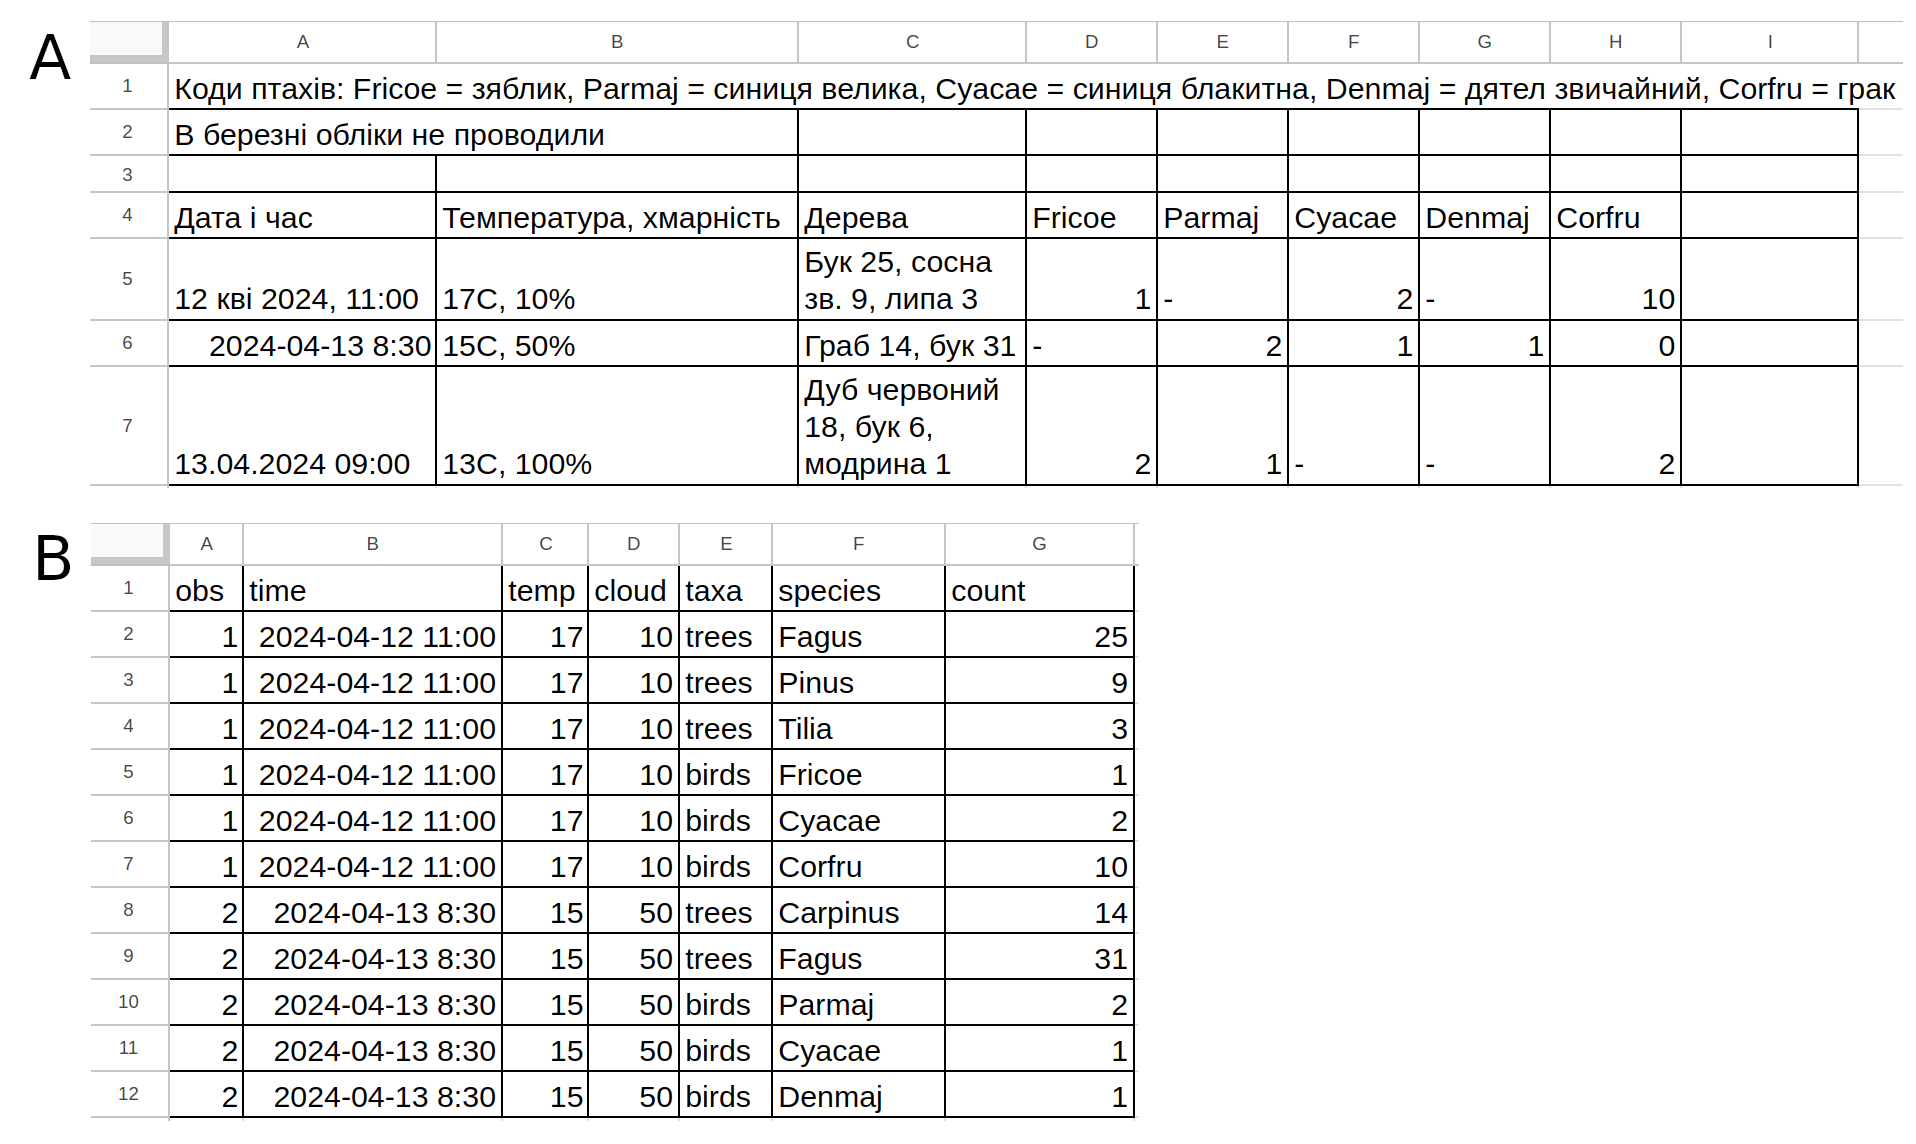
\includegraphics{images/tidydata.png}
\caption{\label{fig:fig-3-14}Уявімо дослідження ефекту структури лісу на населення птахів. Приклад \textbf{(А)} відображає дещо невдалий формат даних: шапка документу займає декілька рядків (їх все одно доведеться видалити для подальшої обробки даних, тож пояснення для значень змінних варто тримати в окремому файлі, наприклад, в документації до набору даних), дата й час не однаковому форматі (їх можна вносити як текст аби уникнути автоматичного форматування, а на етапі роботи з даними можна використати функції бібліотеки \texttt{lubridate} для R), температура й хмарність є двома різними змінними із різними одиницями вимірювання (додавання одиниць вимірювання в клітинки перетворить їх вміст в текст, а додавання коми в клітинках стане на заваді адекватного зчитування даних у форматі *.csv), колонка дерев має нефіксовану кількість значень в кожній клітинці. Натомість, ті ж дані можна оцифрувати в межах парадигми охайних даних \textbf{(В)}, при чому декількома способами. Зображений тут спосіб не викличе необхідності перемикати налаштування мови під час аналізу даних, адже назви колонок прописані англійською мовою, а масив даних легко може бути імпортованим в R.}
\end{figure}

Коли говорити про змінні, то дані можуть мати один із багатьох можливих форматів. Одна змінна може мати лише один формат даних, і, скоріш за все, це буде один із наступних:

\begin{itemize}
\item
  \textbf{логічні дані} (\emph{Boolean}), які приймають одне із двох можливих значень (1/0, правда/неправда, True/False);
\item
  \textbf{числові дані} (\emph{numerical}), що можуть включати як континуальні значення (\emph{double}/\emph{float}, наприклад, вага, зріст тощо), так і дискретні числа (\emph{integer}, наприклад, кількість особин);
\item
  \textbf{текст} (\emph{character}), будь-який набір символів який має принаймні один символ, що не є числом (власне, чому не варто додавати одиниці вимірювання до значень, які за своєю природою є числом);
\item
  \textbf{категорійні дані} (\emph{factor}), в яких одне спостереження може приймати одне значення із певного скінченного набору можливих значень (наприклад, вид, стадія життєвого циклу тощо);
\item
  \textbf{дата/час} (\emph{date/time}) є особливим форматом даних із яким треба бути дуже обережним, адже форматування іноді може дивно поводитись (наприклад, автоматично переводитись в дискретну кількість секунд із якогось моменту типу 1970-01-01 00:00:00), а неповні дані бувають неочевидними (наприклад, якщо надано тільки місяць і день, то не завжди вдається вгадати рік); найповнішим форматом є ``YYYY-MM-DDThh:mm:ss+hh:mm'', наприклад, ``2024-10-15T22:43:25-04:00'' каже ``рік 2024, місяць 10, день 15, година 22, хвилина 43, секунда 25, часовий пояс мінус 4 години від стандартного часу UTC''. Часовий пояс варто наводити, адже в багатьох локаціях наявна змінна літнього і зимового часу; альтернативно, можна наводити час за всесвітнім координованим часом (UTC, позначається як ``Z'' від Zulu), як-то для попереднього прикладу ``2024-10-16T02:43:25Z''.
\end{itemize}

Тепер нарешті погляньмо на структуру статистичної моделі. Вся суть моделювання полягає в тому, що дослідник намагається змоделювати певну \textbf{залежну змінну} (\emph{dependent variable}) як функцію однією або декількох незалежних змінних, або \textbf{предикторів} (\emph{predictor}). Для зручності модель можна записати формулою, яка в найпростішій ситуації виглядатиме як

\[y \sim f(x) \Longleftrightarrow y_i = f(x_i) + \epsilon_i\]

де ми намагаємось змоделювати кожне спостереження залежної змінної \(y\) як функцію змінної \(x\) із врахуванням якоїсь статистичної похибки \(\epsilon\).

Відповідно, проблема аналізу даних може становити або проблему \textbf{регресії} (\emph{regression}) якщо залежна змінна має логічні або числові дані, або проблему \textbf{класифікації} (\emph{classification}) якщо залежна змінна є категорійною.

\subsubsection{Регресія}\label{ux440ux435ux433ux440ux435ux441ux456ux44f}

Регресія в найпростішому вигляді відповідає побудуванню прямої лінії в двовимірних координатах (Рис. \ref{fig:fig-3-2}). Таку лінію можна уявити як залежну змінну \(y\) у вигляді функції предиктора \(x\):

\[y \sim x \Longleftrightarrow y_i = \beta_0 + \beta_1 \cdot x_i + \epsilon_i\]

і в такому разі оцінка коефіцієнтів регресії \(\beta_0\) (інтерцепт, intercept) та \(\beta_1\) (нахил, slope) надасть уявлення про залежність між змінними: якщо \(\beta_1 > 0\), то \(y\) збільшується зі збільшенням \(x\), якщо \(\beta_1 < 0\) -- то існує негативний взаємозв'язок, а статистичне тестування можна зав'язати на нульовій гіпотезі що \(\beta_1 = 0\).

Корисною особливістю лінійної регресії є те, що її можна використати і для моделювання нелінійних залежностей. Наприклад, якщо ми введемо нову змінну \(u\), яка є нелінійною функцією \(x\), скажімо, \(u = x^2\), то нічого не заважає побудувати лінійну регресію

\[y \sim u \Longleftrightarrow y_i = \beta_0 + \beta_1 \cdot u_i + \epsilon_i\]

хоча варто мати на увазі, що \textbf{поліноміальні} (\emph{polynomial}) функції є складнішими, тож, наприклад, моделювання поліноміального зв'язку третього порядку матиме вигляд

\[y \sim \text{poly}(x, 3) \Longleftrightarrow y_i = \beta_0 + \beta_1 \cdot x_i + \beta_2 \cdot x_i^2 + \beta_3 \cdot x_i^3 + \epsilon_i\]

Крім того, можливо також не обмежувати себе одним предиктором і моделювати залежну змінну за допомогою декількох предикторів. Така регресія зветься \textbf{множинною} (\emph{multiple regression}) і дозволяє оцінити ефект (=коефіцієнт) для кожного предиктора окремо якщо між предикикторами немає взаємної кореляції (\emph{multicollinearity}):

\[y \sim a + b + c \Longleftrightarrow y_i = \beta_0 + \beta_1 \cdot a_i + \beta_2 \cdot b_i + \beta_3 \cdot c_i + \epsilon_i\]

Іншими двома важливими припущеннями базових методів регресії є те, що в моделі відсутня \textbf{гетероскедастичність} (\emph{heteroscedasticity}) -- варіація залежної змінної повинна бути незалежною від предикторів, -- і те, що розподіл помилки \(\epsilon\) є нормальним. Простіші регресійні підходи застосовують \hyperref[mle]{метод максимальної правдоподібності} для оцінки таких значень коефіцієнтів регресії, за яких сума квадратів помилок \(\epsilon_i\) є мінімальною, і відтак метод іноді називають \textbf{простою регресією найменших квадратів} (\emph{ordinary least squares regression}, \textbf{\emph{OLS regression}}). Іноді залежна змінна є не континуальною, а, скажімо, логічною (тобто 0/1) або має один із дискретних розподілів (наприклад, Пуасона). В таких випадках в нагоді стають \textbf{узагальнені лінійні моделі} (\emph{generalized linear models}, \textbf{\emph{GLM}}). Існують також методи, які дозволяють будувати криві, які локально підбудовують себе під точки спостережень, однак не мають чітко визначених параметрів і використовуються переважно для візуалізації: \textbf{узагальнені додатні моделі} (\emph{generalized additive models}, \textbf{\emph{GAM}}) та \textbf{локально зважені поліноміальні моделі} (\emph{locally estimated scatterplot smoothing, local regression}, \textbf{\emph{LOESS}}).

Якщо ж предиктором є не континуальна змінна, а категорійний фактор, така модель являтиме приклад дисперсійного аналізу, або \textbf{аналіз варіації} (\emph{analysis of variance}, \textbf{\emph{ANOVA}}). ANOVA розділяє залежну змінну на групи, що відповідають різним рівням фактора предиктора, і перевірка статистичної гіпотези зводиться до того, чи варіація між групами є більшою за варіацію в межах груп. Якщо так, то це лише каже що принаймні одна група має значуще відмінні значення залежної змінної від інших груп, однак не каже яка саме -- для цього часто застосовують \emph{post hoc} тест \textbf{Тюкі} (\emph{Tukey Honestly Significant Difference test}, \textbf{\emph{Tukey HSD}}). Варто пам'ятати, що технічно ANOVA є окремим випадком OLS-регресії, адже тестування гіпотез в регресії використовує то й же механізм, що аналіз варіації (тест Фішера), а фактор можна зобразити у вигляді декількох бінарних колонок, які відповідають рівням фактору (див. \href{https://mcfromnz.wordpress.com/2011/03/02/anova-type-iiiiii-ss-explained/}{коментар} щодо типів кодування аналізу варіації).

Аби проілюструвати регресію в R, корисним набором даних може бути \texttt{iris} із стандартних супутній даних в пакеті \texttt{datasets}. В цьому наборі даних наведено проміри в см чотирьох морфологічних ознак квіток: довжина (\texttt{*.Length}) та ширина (\texttt{*.Width}) чашолистків (\texttt{Sepal.*}) та пелюсток (\texttt{Petal.*}), виміряні в 50 особин кожного з трьох видів півників (\emph{Iris setosa}, \emph{I. versicolor}, та \emph{I. virginica}). Відтак, дані мають 150 рядків та 5 колонок:

\begin{Shaded}
\begin{Highlighting}[]
\CommentTok{\# замість того, щоб бачити всі дані, погляньмо на перші декілька рядків}
\FunctionTok{head}\NormalTok{(iris)}
\end{Highlighting}
\end{Shaded}

\begin{verbatim}
##   Sepal.Length Sepal.Width Petal.Length Petal.Width Species
## 1          5.1         3.5          1.4         0.2  setosa
## 2          4.9         3.0          1.4         0.2  setosa
## 3          4.7         3.2          1.3         0.2  setosa
## 4          4.6         3.1          1.5         0.2  setosa
## 5          5.0         3.6          1.4         0.2  setosa
## 6          5.4         3.9          1.7         0.4  setosa
\end{verbatim}

\begin{Shaded}
\begin{Highlighting}[]
\CommentTok{\# скільки рядків і колонок?}
\FunctionTok{dim}\NormalTok{(iris)}
\end{Highlighting}
\end{Shaded}

\begin{verbatim}
## [1] 150   5
\end{verbatim}

Побудуймо просту лінійну регресію, в якій \texttt{Sepal.Length} є функцією від \texttt{Petal.Length}:

\begin{Shaded}
\begin{Highlighting}[]
\CommentTok{\# запишемо регресію в об\textquotesingle{}єкт}
\NormalTok{fit\_iris1 }\OtherTok{\textless{}{-}} \FunctionTok{lm}\NormalTok{(Sepal.Length }\SpecialCharTok{\textasciitilde{}}\NormalTok{ Petal.Length, }\AttributeTok{data =}\NormalTok{ iris)}
\CommentTok{\# поглягньмо на коефіцієнти регресії}
\FunctionTok{summary}\NormalTok{(fit\_iris1)}
\end{Highlighting}
\end{Shaded}

\begin{verbatim}
## 
## Call:
## lm(formula = Sepal.Length ~ Petal.Length, data = iris)
## 
## Residuals:
##      Min       1Q   Median       3Q      Max 
## -1.24675 -0.29657 -0.01515  0.27676  1.00269 
## 
## Coefficients:
##              Estimate Std. Error t value Pr(>|t|)    
## (Intercept)   4.30660    0.07839   54.94   <2e-16 ***
## Petal.Length  0.40892    0.01889   21.65   <2e-16 ***
## ---
## Signif. codes:  0 '***' 0.001 '**' 0.01 '*' 0.05 '.' 0.1 ' ' 1
## 
## Residual standard error: 0.4071 on 148 degrees of freedom
## Multiple R-squared:   0.76,  Adjusted R-squared:  0.7583 
## F-statistic: 468.6 on 1 and 148 DF,  p-value: < 2.2e-16
\end{verbatim}

Виглядає, що регресію можна описати лінією \(y = 4.307 + 0.409 \cdot x\). Перевірмо, наскільки добре це описує дані:

\begin{Shaded}
\begin{Highlighting}[]
\CommentTok{\# намалюймо точки даних}
\FunctionTok{plot}\NormalTok{(iris}\SpecialCharTok{$}\NormalTok{Petal.Length, iris}\SpecialCharTok{$}\NormalTok{Sepal.Length, }
     \AttributeTok{xlab =} \StringTok{"Petal Length, cm"}\NormalTok{, }\AttributeTok{ylab =} \StringTok{"Sepal Length, cm"}\NormalTok{, }
     \AttributeTok{pch =} \DecValTok{16}\NormalTok{)}
\CommentTok{\# промалюймо лінію регресії}
\FunctionTok{abline}\NormalTok{(}\AttributeTok{a =} \FloatTok{4.3066}\NormalTok{, }\AttributeTok{b =} \FloatTok{0.40892}\NormalTok{, }\AttributeTok{col =} \StringTok{"red"}\NormalTok{)}
\end{Highlighting}
\end{Shaded}

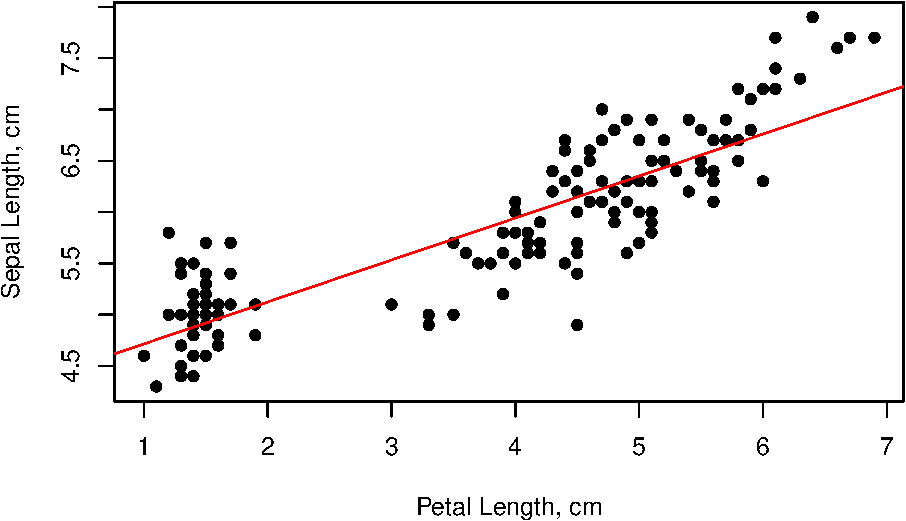
\includegraphics{bookdown-demo_files/figure-latex/unnamed-chunk-19-1.pdf}

Подібним чином можна побудувати й множинну регресію (напр., \texttt{lm(Sepal.Length\ \textasciitilde{}\ Petal.Length\ +\ Petal.Width,\ data\ =\ iris)}), й усіляко досліджувати лінійні та криволінійні взаємозалежності. Завжди варто мати на увазі, втім, що наявність статистично значущих зв'язків не передбачає причинно-наслідкових зв'язків. Наприклад, чи можна справді вважати що довжина пелюсток визначає довжину чашолистків? Натомість, мабуть, біологічно обґрунтованим стало би припущення, що на обидві ці морфологічні ознаки впливають одні й ті ж довкіллєві чи генетичні фактори\footnote{Зручним уявним експериментом для прикладу абсурдності ототожнювання кореляцій (чи інших статистичних зв'язків) та каузацій є наступна ситуація: нескладно уявити, що кількість пожежників, залучених до гасіння пожеж, позитивно пов'язана зі збитками від пожежі -- то чи значить це, що пожежники завдають збитків?}.

\subsubsection{Класифікація}\label{ux43aux43bux430ux441ux438ux444ux456ux43aux430ux446ux456ux44f}

Що ж робити, якщо залежна змінна в моделі є не континуальною, а фактором? Наприклад, чи можна за комбінацією морфологічних промірів квітки передбачити вид півників? Таке завдання відповідатиме проблемі класифікації.

Класифікаційна модель отримує на вхід набір дескрипторів репліканта (рядку даних), і на підставі цих даних намагається оцінити ймовірності того, що об'єкт належить до певного \emph{класу}, наприклад, для трьох видів півників,

\[
\begin{cases}
    P(y_i \in \text{setosa}) = f(x_i) \\
    P(y_i \in \text{versicolor}) = f(x_i) \\
    P(y_i \in \text{virginica}) = f(x_i)
\end{cases}
\]

При чому варто очікувати, що \(P(y_i \in \text{setosa}) + P(y_i \in \text{versicolor}) + P(y_i \in \text{virginica}) = 1\).

Існує чимало алгоритмів класифікації, і не всі з них напряму обчислюють ймовірності, але ідея подібна: для кожного рядку даних алгоритм намагається вгадати клас спостереження. Спробуймо використати один із найбільш класичних алгоритмів, \textbf{k-найближчих сусідів} (\emph{k-nearest neighbors}, \textbf{\emph{KNN}}), для класифікації півників. Механізм алгоритму дуже простий: для кожного нового спостереження, KNN дивиться на найближчі \(k\) спостережень і визначає клас нового спостереження як найбільш поширений серед цих \(k\) спостережень. Наприклад, якщо \(k=3\), і ми намагаємось вгадати клас для спостереження, найближчі сусіди якого є двома \emph{setosa} і одним \emph{virginica}, то нове спостереження визначимо як \emph{setosa}.

KNN є прикладом алгоритму \textbf{машинного навчання із учителем} (\emph{supervised machine learning}). Такі алгоритми вимагають вхідного, \emph{навчального}, набору даних із відомою класифікацією (тому й називаються \emph{supervised}), і очікують нових точок даних для застосування щойно навченого класифікатора. Наприклад, для даних \emph{iris}, де маємо 150 спостережень, найбільш доцільним питанням із використанням KNN було би ``от ми маємо нове спостереження із промірами пелюсток та чашолистиків, але ми не знаємо виду -- який це вид?'' Тоді KNN пошукає найближчих сусідів і видасть результат.

Вибір значення \(k\) є наріжним каменем використання цього методу, адже невідомо скільки найближчих сусідів є забагато чи замало для ефективного алгоритму. Значення \(k=3\) і \(k=5\) є доволі поширеними, але довільними. Для виправданого вибору цього параметру, варто проводити \hyperref[crossval]{валідацію} класифікатора, про що поговоримо пізніше.

Іншим застосуванням класифікатора може бути поділ простору параметрів. Справа в тім, що один класифікатор, навчений на скінченній кількості спостережень, теоретично можна використати для класифікації незліченної кількості точок, а відтак і прокласифікувати цілий простір замість декількох точок. Наприклад, погляньмо на двовимірний простір промірів пелюсток півників.

\begin{Shaded}
\begin{Highlighting}[]
\CommentTok{\# намалюймо точки даних}
\NormalTok{iris }\SpecialCharTok{\%\textgreater{}\%}
  \FunctionTok{ggplot}\NormalTok{(}\FunctionTok{aes}\NormalTok{(}\AttributeTok{x =}\NormalTok{ Petal.Width, }\AttributeTok{y =}\NormalTok{ Petal.Length, }\AttributeTok{color =}\NormalTok{ Species)) }\SpecialCharTok{+}
  \FunctionTok{geom\_point}\NormalTok{()}
\end{Highlighting}
\end{Shaded}

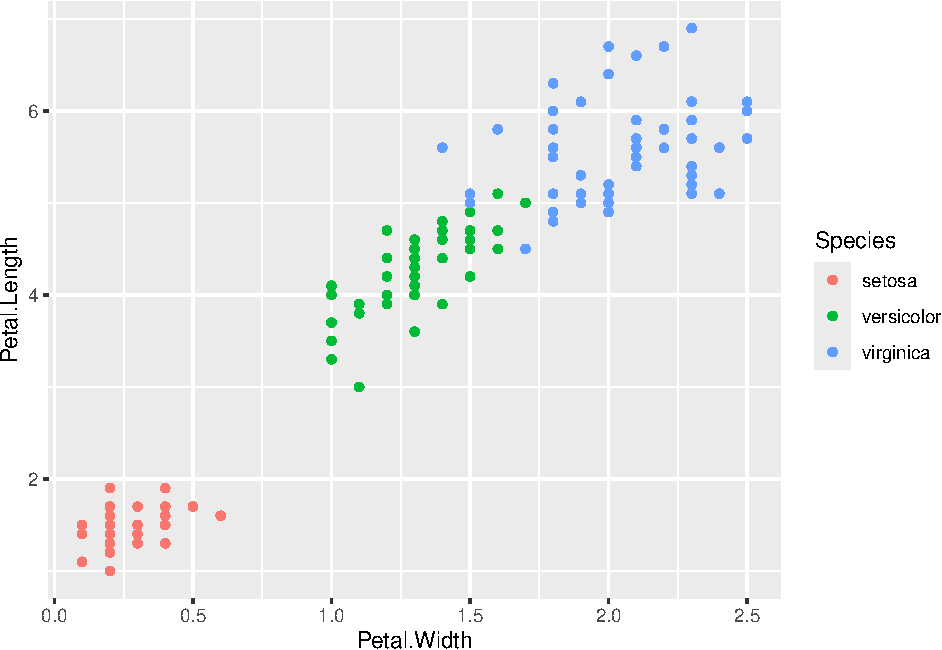
\includegraphics{bookdown-demo_files/figure-latex/unnamed-chunk-20-1.pdf}

\begin{Shaded}
\begin{Highlighting}[]
\CommentTok{\# побудуємо KNN класифікатор із k = 5}
\FunctionTok{library}\NormalTok{(caret)}
\end{Highlighting}
\end{Shaded}

\begin{verbatim}
## Loading required package: lattice
\end{verbatim}

\begin{verbatim}
## 
## Attaching package: 'caret'
\end{verbatim}

\begin{verbatim}
## The following object is masked from 'package:purrr':
## 
##     lift
\end{verbatim}

\begin{Shaded}
\begin{Highlighting}[]
\NormalTok{fit\_iris2 }\OtherTok{\textless{}{-}}\NormalTok{ caret}\SpecialCharTok{::}\FunctionTok{train}\NormalTok{(Species }\SpecialCharTok{\textasciitilde{}}\NormalTok{ Petal.Width }\SpecialCharTok{+}\NormalTok{ Petal.Length, }
                   \AttributeTok{data =}\NormalTok{ iris, }
                   \AttributeTok{method =} \StringTok{"knn"}\NormalTok{, }
                   \AttributeTok{tuneGrid =} \FunctionTok{data.frame}\NormalTok{(}\AttributeTok{k =} \DecValTok{5}\NormalTok{))}

\CommentTok{\# генерація точок в просторі параметру}
\NormalTok{xg }\OtherTok{\textless{}{-}} \FunctionTok{seq}\NormalTok{(}\FunctionTok{min}\NormalTok{(iris}\SpecialCharTok{$}\NormalTok{Petal.Width), }\FunctionTok{max}\NormalTok{(iris}\SpecialCharTok{$}\NormalTok{Petal.Width), }\AttributeTok{length.out =} \DecValTok{100}\NormalTok{)}
\NormalTok{yg }\OtherTok{\textless{}{-}} \FunctionTok{seq}\NormalTok{(}\FunctionTok{min}\NormalTok{(iris}\SpecialCharTok{$}\NormalTok{Petal.Length), }\FunctionTok{max}\NormalTok{(iris}\SpecialCharTok{$}\NormalTok{Petal.Length), }\AttributeTok{length.out =} \DecValTok{100}\NormalTok{)}
\NormalTok{xyg }\OtherTok{\textless{}{-}} \FunctionTok{expand.grid}\NormalTok{(xg, yg)}
\FunctionTok{colnames}\NormalTok{(xyg) }\OtherTok{\textless{}{-}} \FunctionTok{c}\NormalTok{(}\StringTok{"Petal.Width"}\NormalTok{, }\StringTok{"Petal.Length"}\NormalTok{)}

\CommentTok{\# застосуємо і запишемо класифікацію нових точок}
\NormalTok{xyg}\SpecialCharTok{$}\NormalTok{Species }\OtherTok{\textless{}{-}} \FunctionTok{predict}\NormalTok{(fit\_iris2, xyg)}

\CommentTok{\# промалюємо простір}
\FunctionTok{ggplot}\NormalTok{() }\SpecialCharTok{+}
   \FunctionTok{geom\_raster}\NormalTok{(}\AttributeTok{data =}\NormalTok{ xyg,}
               \FunctionTok{aes}\NormalTok{(}\AttributeTok{x =}\NormalTok{ Petal.Width, }\AttributeTok{y =}\NormalTok{ Petal.Length, }\AttributeTok{fill =}\NormalTok{ Species),}
               \AttributeTok{alpha =} \FloatTok{0.5}\NormalTok{) }\SpecialCharTok{+}
  \FunctionTok{geom\_point}\NormalTok{(}\AttributeTok{data =}\NormalTok{ iris,}
             \FunctionTok{aes}\NormalTok{(}\AttributeTok{x =}\NormalTok{ Petal.Width, }\AttributeTok{y =}\NormalTok{ Petal.Length, }\AttributeTok{color =}\NormalTok{ Species))}
\end{Highlighting}
\end{Shaded}

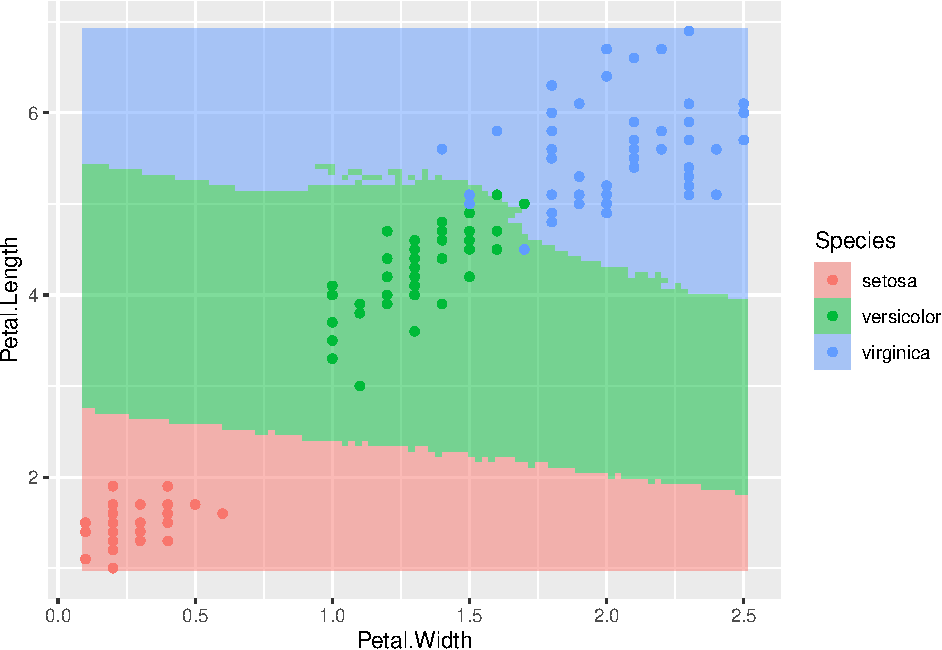
\includegraphics{bookdown-demo_files/figure-latex/unnamed-chunk-20-2.pdf}

Цікаво, що KNN можна застосувати і до проблеми регресії, якщо залежна змінна є континуальною. В такому випадку, класифікатор шукатиме середнє значення (або іншу статистику) для \(k\) найближчих сусідів.

Загалом же, існує чимало інших алгоритмів класифікації. Деякі із них кластеризують точки без вхідних даних щодо класів спостережень і є, відтак, алгоритмами машинного навчання \emph{без учителя} (\emph{unsupervised machine learning}) -- наприклад, метод \textbf{K-середніх} (\emph{K-means}), який ітеративно шукає найкращий поділ хмари точок на \(K\) кластерів. Тема машинного навчання є дуже популярною, й, відтак, нові алгоритми з'являються доволі часто.

\subsection{Парсимонійна модель та вибір моделі}\label{aic}

\subsection{Багатовимірна статистика}\label{prcomp}

\section{Використання статистики для умовиводу}\label{infer}

\subsection{Статистичний умовивід і обґрунтоване передбачення}\label{inference}

\subsection{Крос-валідація}\label{crossval}

\chapter{Початки популяційної екології}\label{popeco}

\section{Вид}\label{species}

\section{Популяція}\label{population}

\section{Метапопуляція}\label{metapopulation}

\section{Чинники, що впливають на популяції}\label{pop-factors}

\section{Внутрішньовидові взаємодії}\label{intraspecific}

\section{Динаміка та стабільність}\label{pop-dynamics}

\section{Матриці Леслі}\label{Leslie-matrix}

\chapter{Фундаментальні поняття екології}\label{foundations}

\section{Екологічна ніша}\label{niche}

\section{Трофічні ланцюги}\label{food-chain}

\section{Трофічні мережі}\label{food-webs}

\section{Ключові види}\label{keystones}

\section{Сукцесія та клімакс}\label{succession}

\section{Історія життя}\label{life-history}

\section{Ймовірність детекції}\label{detectability}

\chapter{Міжвидові взаємодії}\label{interspecific}

\section{Типи міжвидових зв'язків}\label{relationships}

\section{Теорія поділу ресурсів}\label{rstar}

\section{Трофічні каскади}\label{cascade}

\chapter{Екологічні угруповання}\label{comecol}

\section{Структура угруповання}\label{sad}

\section{Моделі розподілів чисельності}\label{sad-model}

\section{Різноманіття}\label{diversity}

\section{Подібність угруповань}\label{similarity}

\section{Функціональне й філогенетичне різноманіття}\label{fd}

\section{Острівна біогеографія}\label{islands}

\section{Середовищне фільтрування}\label{env-filter}

\section{Рарефакція та екстраполяція}\label{rarefaction}

\chapter*{Післяслово}\label{ux43fux456ux441ux43bux44fux441ux43bux43eux432ux43e}
\addcontentsline{toc}{chapter}{Післяслово}

\chapter*{Контакти автора}\label{ux43aux43eux43dux442ux430ux43aux442ux438-ux430ux432ux442ux43eux440ux430}
\addcontentsline{toc}{chapter}{Контакти автора}

Найкращий спосіб -- електронна пошта \href{mailto:oadubovyk@gmail.com}{\nolinkurl{oadubovyk@gmail.com}}

Листи невимовного захвату вкриті нестримними сльозами радості від читання посібника надсилати за адресою:

Oleksii Dubovyk, PhD Student

Dept Biol Sci, Mills Godwin Bldg 110

Old Dominion University, Norfolk, VA

23529, USA

  \bibliography{book.bib,packages.bib}

\end{document}
